\documentclass[12pt,a4paper,twoside,openany]{report} %openright
\let\openright=\cleardoublepage



%%% Choose a language %%%

\newif\ifEN
\ENtrue   % uncomment this for english
%\ENfalse   % uncomment this for czech

%%% Configuration of the title page %%%

\def\ThesisTitleStyle{mff} % MFF style
%\def\ThesisTitleStyle{cuni} % uncomment for old-style with cuni.cz logo
%\def\ThesisTitleStyle{natur} % uncomment for nature faculty logo

\def\UKFaculty{Faculty of Mathematics and Physics}
%\def\UKFaculty{Faculty of Science}

\def\UKName{Charles University in Prague} % this is not used in the "mff" style

% Thesis type names, as used in several places in the title
\def\ThesisTypeTitle{\ifEN BACHELOR THESIS \else BAKALÁŘSKÁ PRÁCE \fi}
%\def\ThesisTypeTitle{\ifEN MASTER THESIS \else DIPLOMOVÁ PRÁCE \fi}
%\def\ThesisTypeTitle{\ifEN RIGOROUS THESIS \else RIGORÓZNÍ PRÁCE \fi}
%\def\ThesisTypeTitle{\ifEN DOCTORAL THESIS \else DISERTAČNÍ PRÁCE \fi}
\def\ThesisGenitive{\ifEN bachelor \else bakalářské \fi}
%\def\ThesisGenitive{\ifEN master \else diplomové \fi}
%\def\ThesisGenitive{\ifEN rigorous \else rigorózní \fi}
%\def\ThesisGenitive{\ifEN doctoral \else disertační \fi}
\def\ThesisAccusative{\ifEN bachelor \else bakalářskou \fi}
%\def\ThesisAccusative{\ifEN master \else diplomovou \fi}
%\def\ThesisAccusative{\ifEN rigorous \else rigorózní \fi}
%\def\ThesisAccusative{\ifEN doctoral \else disertační \fi}



%%% Fill in your details %%%

% (Note: \xxx is a "ToDo label" which makes the unfilled visible. Remove it.)
\def\ThesisTitle{Financial News Sentiment Analysis}
\def\ThesisAuthor{Václav Stibor}
\def\YearSubmitted{2024}

% department assigned to the thesis
\def\Department{Department of Software Engineering}
% Is it a department (katedra), or an institute (ústav)?
\def\DeptType{Department}

\def\Supervisor{doc. RNDr. Irena Holubová, Ph.D.}
\def\SupervisorsDepartment{Department of Software Engineering}

% Study programme and specialization
\def\StudyProgramme{Computer Science}
\def\StudyBranch{\xxx{study branch}}

\def\Dedication{%
    I would like to dedicate this thesis to my family and friends who have supported me throughout my studies. Special thanks to my supervisor doc. RNDr. Irena Holubová, Ph.D. for her expertise and guidance during the development of this work. To all who have assisted me, I sincerely appreciate your support.

    Additionally, I am grateful for the consultations provided by Mgr. Petr Škoda, Ph.D., and Ing. Pavel Koupil, Ph.D. contributed to this thesis's improved outcomes.
}

\def\AbstractEN{%
{
    In the current era of information overload, tracking associations and comprehending media and online news content, especially for investment purposes, is becoming increasingly demanding. This thesis addresses the challenge by developing an application that evaluates sentiment analysis and visualises connections between companies and news articles. The cornerstone of the application is the extraction of data from news articles, sentiment analysis of the extracted entities, and the provision of this information as an indicator of potential future influences on a company's stock price. The application is designed to be easy to use and intuitive, allowing users to navigate to the articles and perform their analysis to verify the values provided by the application.
}
% ABSTRACT IS NOT A COPY OF YOUR THESIS ASSIGNMENT! < 500 Words
}

\def\AbstractCS{%
V dnešní době přehlcené informacemi se sledování souvislostí a porozumění obsahu médií a online zpráv, zejména pro investiční účely, se stává stále náročnějším. Tato práce se zabývá daným problémem a vývojem aplikace, která vyhodnocuje analýzu sentimentu a vizualizuje spojení mezi společnostmi a zpravodajskými články. Základem aplikace je extrakce dat ze zpravodajských článků, analýza sentimentu extrahovaných entit a poskytování těchto informací jako indikátor možných budoucích vlivů na cenu akcií společnosti. Aplikace je navržena tak, aby byla snadno použitelná a intuitivní, což umožňuje uživatelům navigovat k článkům a provádět tak i vlastní analýzu pro ověření hodnot poskytovaných aplikací.
}

%\xxx{You will need to submit both Czech and English abstract to the SIS, no matter what language you use in the thesis. If writing in English, translate the contents of \texttt{\textbackslash{}AbstractEN} into this field. In case you do not speak czech, your supervisor should be able to help you with the translation.}

% 3 to 5 keywords (recommended), each enclosed in curly braces.
% Keywords are useful for indexing and searching for the theses by topic.
\def\Keywords{%
{entity-level} {sentiment analysis} {news} {stock market}
}

% If your abstracts are long and do not fit in the infopage, you can make the
% fonts a bit smaller by this setting. (Also, you should try to compress your abstract more.)
% Alternatively, consider increasing the size of the page by uncommenting the
% geometry modification in thesis.tex.
\def\InfoPageFont{}
%\def\InfoPageFont{\small}  %uncomment to decrease font size

\ifEN\relax\else
% If you are writing a czech thesis, you additionally need to fill in the
% english translation of the metadata here!
\def\ThesisTitleEN{\xxx{Thesis title in English}}
\def\DepartmentEN{\xxx{Name of the department in English}}
\def\DeptTypeEN{\xxx{Department}}
\def\SupervisorsDepartmentEN{\xxx{Superdepartment}}
\def\StudyProgrammeEN{\xxx{study programme}}
\def\StudyBranchEN{\xxx{study branch}}
\def\KeywordsEN{%
\xxx{{key} {words}}
}
\fi


\usepackage[a-2u]{pdfx}

\ifEN\else\usepackage[czech,shorthands=off]{babel}\fi
\usepackage[utf8]{inputenc}
\usepackage[T1]{fontenc}
\usepackage{lmodern}

% See https://en.wikipedia.org/wiki/Canons_of_page_construction before
% modifying the size of printable area. LaTeX defaults are great. 
% If you feel it would help anything, you can enlarge the printable area a bit:
%\usepackage[textwidth=390pt,textheight=630pt]{geometry}
% The official recommendation expands the area quite a bit (looks pretty harsh):
%\usepackage[textwidth=145mm,textheight=247mm]{geometry}

%%% FONTS %%%
%\usepackage{libertinus} % popular for comp-sci (ACM uses this) false

%\usepackage{libertinus}
%\usepackage{tgschola} 
%\usepackage[scale=0.96]{tgpagella}

% Optionally choose an override for the main font for typesetting:
%\!!!!!usepackage[mono=false]{libertinus} % popular for comp-sci (ACM uses this)
%\usepackage{tgschola} % Schoolbook-like (gives a bit of historic feel)
%\usepackage[scale=0.96]{tgpagella} %  Palladio-like (popular in formal logic).
% IBM Plex font suite is nice but requires us to fine-tune the sizes, also note
% that it does not directly support small caps (\textsc) and requires lualatex:
%\usepackage[usefilenames,RM={Scale=0.88},SS={Scale=0.88},SScon={Scale=0.88},TT={Scale=0.88},DefaultFeatures={Ligatures=Common}]{plex-otf}

% Optionally choose a custom sans-serif fonts (e.g. for figures and tables).
% Default sans-serif font is usually Latin Modern Sans. Some font packages
% (e.g. libertinus) replace that with a better matching sans-serif font.
%\usepackage{tgheros} % recommended and very readable (Helvetica-like)
%\usepackage{FiraSans} % looks great
% DO NOT typeset the main text in sans-serif font!
% The serifs make the text easily readable on the paper.

% IMPORTANT FONT NOTE: Some fonts require additional PDF/A conversion using
% the pdfa.sh script. These currently include only 'tgpagella'; but various
% other fonts from the texlive distribution need that too (mainly the Droid
% font family).


% some useful packages
\usepackage{multirow} % multirow cells in tables added by Vaclav Stibor
\usepackage{microtype}
\usepackage{amsmath,amsfonts,amsthm,bm}
\usepackage{graphicx}
\usepackage{xcolor}
\usepackage{booktabs}
\usepackage{caption}
\usepackage{floatrow}
\usepackage{titlesec}
\titleformat{\chapter}[hang] 
{\normalfont\huge\bfseries}{\thechapter.}{0.5em}{}
\titlespacing*{\chapter}{0pt}{0pt}{20pt}
% load bibliography tools
\usepackage[backend=bibtex,natbib,style=authoryear,maxnames=1,sorting=none]{biblatex}
%\usepackage[backend=biber, style=alphabetic, giveninits=true, maxnames=10, sorting=none, articlein=false]{biblatex}
\DeclareFieldFormat*{title}{\emph{#1}} % italic title without quotation marks
\DeclareFieldFormat*{citetitle}{\emph{#1\isdot}} % italic title without quotation marks
\DeclareCiteCommand{\citetitle}
  {\boolfalse{citetracker}%
   \boolfalse{pagetracker}%
   \usebibmacro{prenote}}
  {\ifciteindex
     {\indexfield{indextitle}}
     {}%
   \printtext[bibhyperref]{\printfield[citetitle]{labeltitle}}}
  {\multicitedelim}
  {\usebibmacro{postnote}}
% alternative with alphanumeric citations (more informative than numbers):
%\usepackage[backend=bibtex,natbib,style=alphabetic]{biblatex}
%
% alternatives that conform to iso690
% (iso690 is not formally required on MFF, but may help elsewhere):
%\usepackage[backend=bibtex,natbib,style=iso-numeric,sorting=none]{biblatex}
%\usepackage[backend=bibtex,natbib,style=iso-alphabetic]{biblatex}
%
% additional option choices:
%  - add `giveninits=true` to typeset "E. A. Poe" instead of full Edgar Allan
%  - `terseinits=true` additionaly shortens it to nature-like "Poe EA"
%  - add `maxnames=10` to limit (or loosen) the maximum number of authors in
%    bibliography entry before shortening to `et al.` (useful when referring to
%    book collections that may have hundreds of authors)
%  - for additional flexibility (e.g. multiple reference sections, etc.),
%    remove `backend=bibtex` and compile with `biber` instead of `bibtex` (see
%    Makefile)
%  - `sorting=none` causes the bibliography list to be ordered by the order of
%    citation as they appear in the text, which is usually the desired behavior
%    with numeric citations. Additionally you can use a style like
%    `numeric-comp` that compresses the long lists of citations such as
%    [1,2,3,4,5,6,7,8] to simpler [1--8]. This is especially useful if you plan
%    to add tremendous amounts of citations, as usual in life sciences and
%    bioinformatics.
%  - if you don't like the "In:" appearing in the bibliography, use the
%    extended style (`ext-numeric` or `ext-alphabetic`), and add option
%    `articlein=false`.
%
% possibly reverse the names of the authors with the default styles:
%\DeclareNameAlias{default}{family-given}

% load the file with bibliography entries
\addbibresource{refs}

\let\originalIncludegraphics\includegraphics

% Redefine the \includegraphics command to include interpolate=false
\renewcommand{\includegraphics}[2][]{%
  \originalIncludegraphics[#1,interpolate=false]{#2}%
}

% load the glossary entries
\usepackage[acronym]{glossaries}

\loadglsentries{acronyms}

% remove this if you won't use fancy verbatim environments
\usepackage{fancyvrb}

% remove this if you won't typeset TikZ graphics
\usepackage{tikz}
\usetikzlibrary{positioning} %add libraries as needed (shapes, decorations, ...)

% remove this if you won't typeset any pseudocode
\usepackage{algpseudocode}
\usepackage{algorithm}
%\usepackage{algorithm2e}
%\RestyleAlgo{ruled}

% remove this if you won't list any source code 
\usepackage{listings}


\hypersetup{unicode}
\hypersetup{breaklinks=true}

% New environment for changemargin - used for the description items
\newenvironment{changemargin}[2]{\begin{list}{}{\setlength{\topsep}{0pt}\setlength{\leftmargin}{#1}\setlength{\rightmargin}{#2}\setlength{\listparindent}{\parindent}\setlength{\itemindent}{\parindent}\setlength{\parsep}{\parskip}}\item[]}{\end{list}}

\usepackage[noabbrev]{cleveref}
\usepackage{graphicx}
\usepackage{subcaption}

\input{todos} % remove this before compiling the final version

\input{macros} % use this file for various custom definitions


\begin{document}

\include{title}

\tableofcontents


\chapwithtoc{Introduction}

In today's era of information explosion and constant flow of information, it becomes more time-consuming to keep track of associations and deeply understand the published content through media and online news, primarily when investing in a specific area. For instance, the investment in a company like Apple~Inc. requires acquiring and processing a wide range of available information with significant effort and dedication in studying articles and other sources. At the same time, publicly available information resources such as news articles and tools like sentiment analysis allow us to transfer real-world context into the digital environment and use it for our benefit.

Sentiment analysis, the ability to identify and evaluate the emotional charge of content, has evolved into a crucial instrument for comprehending opinions and the general atmosphere surrounding various topics. This work focuses on developing an application that allows users to visualise connections between companies and news articles using a graph network and the impact of news sentiment on~a company's stock price.

Many experiments are currently being conducted based on historical data to examine the effect of sentiment, with promising results on datasets. The absence of such an application motivates this thesis. An application that extracts actual data from news for sentiment analysis and subsequently provides this information as an indicator of the future possible influence of a company's stock price.

One potential reason for the absence of such an application may be working with a constant flow of updating data, which can present a challenge to creating a functional application. Due to the valuable nature of news sources as information providers, they protect their data against similar usage. Despite the public availability of this data, legal complications may arise from potential violations of terms and conditions, as presented in the OpenAI, Microsoft and The New York Times dispute outlined in Chapter \ref{chap:textual-data}.

Another reason is that this is still an experimental technology and a speculative approach to the market. These technologies are still evolving, and there is no clear-cut approach to $100\%$ stock price prediction depending on news. Nevertheless, published studies involving experiments suggest correlations impact between stock prices and news data. Another notable aspect is shown in Figure \ref{fig:apple-intro}, indicating the correlation between the number of news mentioning a company and its market price. Although it may be less than $100\%$ accurate in prediction, it is an exciting topic that can be very useful for examining the impact on prices and providing an overview of the situation.
 
\begin{figure}[htbp]
    \centering
    \includegraphics[width=\textwidth]{img/intro/apple-intro-a.pdf}
    \caption{Apple Inc. (AAPL) adjusted close price and the volume of news mentions in the Guardian's business and technology section in the first quarter of 2023.}
    \label{fig:apple-intro}
\end{figure}

Providing users with high-quality and reliable data is essential. Therefore, we will source data from trusted and verified newspapers and data providers. Additionally, we need to develop our algorithm for processing all data in the pipeline from extraction to recognition entity, analysis of sentiment, and loading to the database, considering there are few applications of this type, especially those focusing on entities, which is the ideal choice in our context.

The thesis is structured as follows: Chapter \ref{chap:theoretical-background} discusses the foundational concepts of sentiment analysis and named entity recognition. In Chapter \ref{chap:related-work}, we review existing applications and their methodologies in sentiment analysis, as well as recent studies related to sentiment analysis at the entity level and stock market behavior. Challenges associated with obtaining data from newspaper sources are addressed in Chapter \ref{chap:textual-data}, while Chapter \ref{chap:comapny-to-symbol-linking} focuses on detecting entities in text and extracting company names with their ticker symbols. In Chapter \ref{chap:entity-level-sentiment-analysis}, we develop an algorithm for entity-level sentiment analysis of the extracted entities and explore how this information can be used for market analysis. After describing the non-functional and functional application requirements in Chapter \ref{chap:application-requirements}, Chapter \ref{chap:architecture} covers the application architecture based on the previous chapters. We present the developer documentation in Chapter \ref{chap:development-documentation}. Chapter \ref{chap:user-documentation} is dedicated to the user documentation. Finally, the conclusion summarizes the results and discusses potential improvements and future application development.
\chapter{Theoretical Background}
\label{chap:theoretical-background}
Since the application's core is sentiment analysis, it is necessary to define the basic concepts. \textcolor{lightgray}{Lorem ipsum dolor sit amet, consectetur adipiscing elit. Sed non risus. Suspendisse lectus tortor, dignissim sit amet, adipiscing nec, ultricies sed, dolor. Lorem ipsum dolor sit amet, consectetur adipiscing elit. Sed non risus. Suspendisse lectus tortor, dignissim sit amet, adipiscing nec, ultricies sed, dolor. Lorem ipsum dolor sit amet, consectetur adipiscing elit. Sed non risus. Suspendisse lectus tortor, dignissim sit amet, adipiscing nec, ultricies sed, dolor. Lorem ipsum dolor sit amet, consectetur adipiscing elit. Sed non risus.}

\section{Sentiment Analysis Basics}
\label{sec:sentiment-analysis-basics}
Sentiment analysis or opinion mining is a subfield of \acrshort{nlp} that aims to identify and extract opinions and emotions from a text. The goal is to determine the author's attitude towards a particular topic or the overall contextual polarity~of various document levels. We measure the text's polarity using a numerical scale ranging from -1 to 1. The low-end score of the scale signifies a negative sentiment, zero represents neutrality, and the high-end score indicates a positive sentiment. This scale effectively estimates the degree of negativity or positivity in the text's tone. 

The extraction of opinions and emotions has applications in various areas, from product reviews to political events. Hence, it is imperative to work in different domains (see \cite{PIRYANI2017122}). Because of cross-domain and cross-language, two of the most general issues in sentiment analysis, this thesis will focus only on the financial domain in English. Nevertheless, domain-specific sentiment analysis achieves remarkable accuracy while staying highly domain-sensitive, as shown \cite{saunders_2020}. To delve deeper into cross issues, \citeauthor{liu2022sentiment} provides further details in his book \citetitle{liu2022sentiment}\todo{(Q-1.1) Zeptat se - nebo je lepší odkaz "in his work Lei, 2022" v context citatce v Bibliography, kde odkazuji na konkrétní strany z jeho knihy, které se daným problémem odkazují.}.

\subsection{Levels of Sentiment Analysis}
\label{subsec:levels-of-sentiment-analysis}
Sentiment analysis has been studied at several levels of granularity: Document-level, Sentence-level, Phrase-level, and Entity-level\footnote{Entities are sometimes referred to as targets, hence Target-level or Target-based sentiment analysis.}, as illustrated in Fig. \ref{fig:sa-levels}.

\begin{figure}[H]
    \centering
    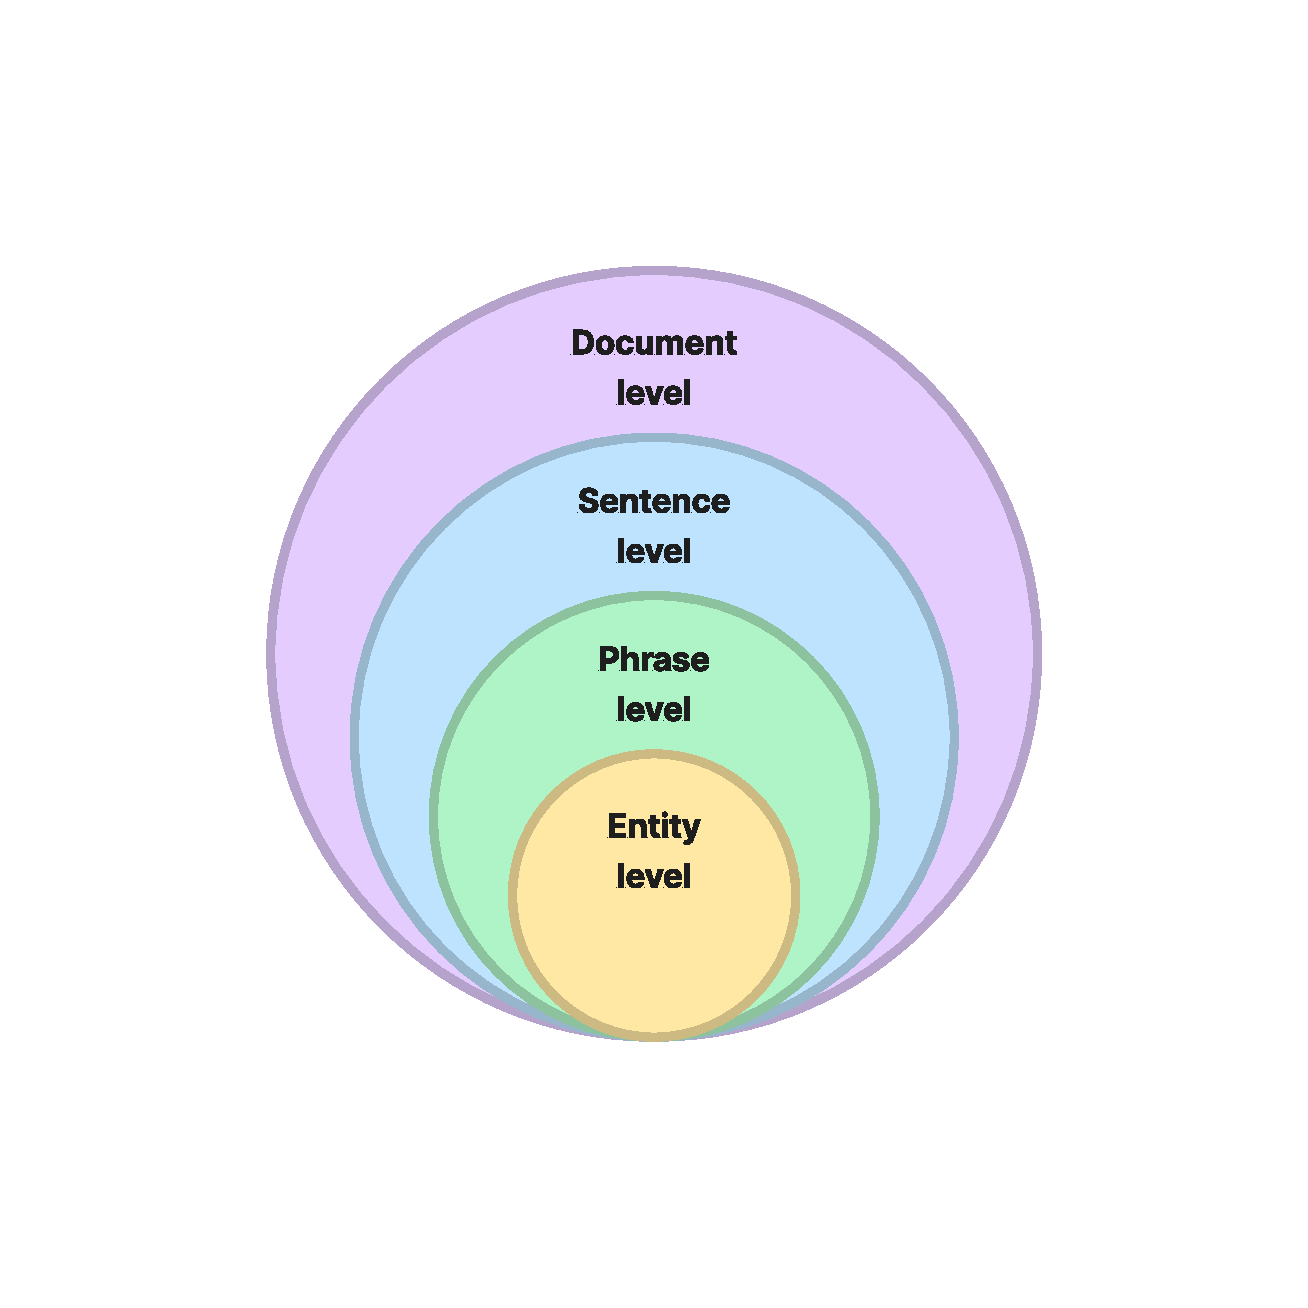
\includegraphics[width=0.5\textwidth]{img/sa-levels.pdf}
    \caption{Levels of sentiment analysis (inspired by \cite{Wankhade2022}).}
    \label{fig:sa-levels}
\end{figure}
\todo{(Q-1.1.1-1) Zeptat se - Je třeba citovat?}

\subsubsection*{Document-level}
\label{subsubsec:document-level}
%At the first level is document-level sentiment analysis. This level is the most straight.
Document-level sentiment analysis is the most straight level. The task is to determine the overall emotional context of the entire document, such as a chapter, article, or review, whether or not involving a study of entities or aspects. This level gives us a general assessment of whether the content is more likely to be positive, negative, or neutral. 

\subsubsection*{Sentence-level}
\label{subsubsec:sentence-level}
Sentiment analysis at the sentence level focuses on individual sentences within the text. We observe the polarity of each sentence autonomously, employing the same methodologies utilized at the document level but with an increased volume of training data and enhanced processing resources. This level is more challenging than the document level because it requires a more in-depth understanding of the text. 

\subsubsection*{Phrase-level}
\label{subsubsec:phrase-level}
Phrase-level sentiment analysis examines sentiment within smaller linguistic units such as phrases or sentence members. Thus, it can better reveal the emotional charge in specific parts of sentences.  Additionally, this level is more challenging than the sentence level because it requires a more detailed understanding of the text. 


\subsubsection*{Entity-level}
\label{subsubsec:entity-level}
The most elaborative level is entity-level sentiment analysis, where we study sentiment associated with specific entities mentioned in the text. This level provides a detailed look at the expressed polarity of certain products, individuals, or organizations. One of the main tasks in this scope is the named entity recognition, which will be discussed later.

\paragraph{}

Some researchers classify the last level as the aspect-level, as noted by \cite{Wankhade2022}, or a more detailed entity-level version called the feature-level proposed by \cite{Jenifer2017}. While both approaches aim to evaluate sentiment towards specific aspects, they differ in their task approach. Relationships between these levels are illustrated in Fig. \ref{fig:enity-feature-aspect-level}.

In the first case, aspects are considered without directly mentioning entities in the text. We are not interested in the entities since the \todo{(Q-1.1.1-2) Zeptat se - Nebo zaměnit "investigated textual data" za "(input) data"?} investigated textual data are commonly associated with them\footnote{Entities are not handled in this case, but we provide them here for a better understanding.}, such as reviews. The study conducted by \cites{Wang2019} analyzed sentiment at the aspect level within restaurant reviews. It primarily examines aspects such as food, price, service, and others. In~the feature-based approach, aspects are commonly associated with an entity's features by connecting the entity and its aspects in text. To illustrate, consider the sentence:\begin{quote}
    \textit{``The battery life of this phone is excellent, but the camera is not good.''}
\end{quote} At the feature level, we identify \textit{the battery life} and \textit{camera} as specific features of entity \textit{the phone}, allowing us to determine the polarity of each entity's feature.

\begin{figure}[H]
    \centering
    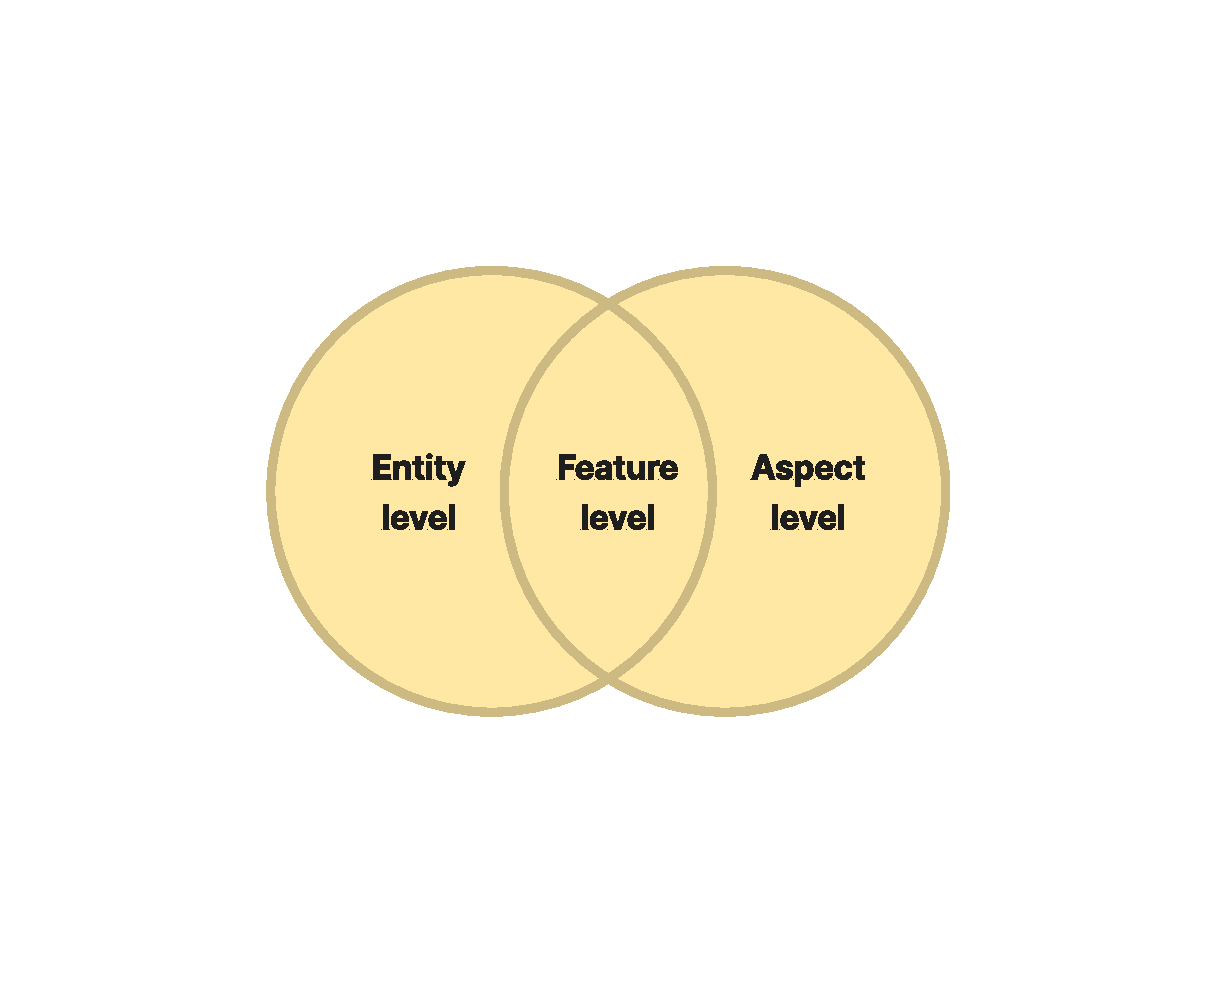
\includegraphics[width=0.5\textwidth]{img/entity-feature-aspect-level.pdf}
    \caption{Comprehensive overview of the last level.}
    \label{fig:enity-feature-aspect-level}
\end{figure}

% Každé rozdělení posledního levelu zkoumáme v rámci předešlých levelů. Toz namneá, že entity level zkoumáme v rámci document, sentence a nebo phrase. Opačně můžeme ale i nemusíme zkoumat document, sentence a nebo phrase v rámci entity levelu.

The term entity-level sentiment analysis is frequently employed in literature, and some studies consider it synonymous with targeted sentiment analysis, \linebreak as discussed \cite{ronningstad-etal-2022-entity} in the terminology review. For our purposes, entity-level sentiment analysis better captures the aggregate, document-wide approach, where a single entity can be associated with multiple targets in different sentences, discerning it from traditional target-level sentiment analysis. 

However, this thesis primarily focuses on entity-level sentiment analysis, excluding consideration of the entity's features. This decision is motivated by treating the mentioned companies in news articles as entities rather than delving into their specific aspects.\todo{TODO: Pokud nenarazím na článek, který by to vyvrátil. Navíc se zkoumáním aspektů by přibylo spousty práce.} Additionally, entity and aspect extraction as separate tasks are complex and challenging, given that the methods \textcolor{lightgray}{and facets} employed for recognition differ due to their distinct characteristics \parencite{Liu2015, Zhang2014}. 

\subsection{Workflow of Sentiment Analysis}
\label{subsec:workflow-of-sentiment-analysis}
The sentiment analysis process can be divided into three main steps: data retrieval, preprocessing, and analysis. The following sections will discuss these steps in more detail.

\section{Named Entity Recognition}
\label{sec:named-entity-recognition}
We will focus on the named entity recognition, also known as entity extraction, in the context of news. 
% Good survey https://wandb.ai/madhana/Named_Entity_Recognition/reports/A-Beginner-s-Guide-to-Named-Entity-Recognition-NER---VmlldzozNjE2MzI1
Named entity recognition is a subtask of \acrshort{nlp} with a focus on identifying and classifying named entities in text into predefined categories such as the names of organizations, persons, locations, expressions of times, quantities, monetary values, and so on. Named entity recognition is a crucial step in entity-level sentiment analysis, as it allows us to identify the sentiment associated with specific entities mentioned in the text. \textcolor{lightgray}{And so on...} %In a given text, there could be several mentions of separate entities, each possibly referred to directly and indirectly multiple times, with varying polarities.

\section{Time Series Forecasting Integration}
\label{sec:integration-with-time-series-forecasting-for-market-trends}
We will focus on integrating time series forecasting in the context of news.

\todo{(Q-1.3) Zeptat se - Bude třeba úvod do stock marketu? Podle mě ne a zbytečně by se to míchalo do (technology) teoretického pozadí.}
\chapter{Data}
\label{chap:data}

Newspaper articles play a key role in our web application. We must consider several essential aspects to integrate these data into our web application to ensure a smooth and effective implementation. The following chapter will discuss these aspects from different perspectives, including the programmer's viewpoint and legislative considerations. \todo{In section X.X. we will give an overview...}

For our entity-level sentiment proposes, we need a body of each article as we discuss in Chapter \ref{chap:theoretical-background} \todo{refer to chapter Related Works, where we discuss maybe why others work only with titles}. 
When selecting data source of news article, it is essential to consider several main aspects.

\begin{table}[htbp]
    \caption{Considerations for Selecting News Article Data Source}
    \centering
    \begin{tabular}{p{0.3\linewidth}p{0.5\linewidth}}
        \toprule
        \textbf{Aspect} & \textbf{Description} \\
        \midrule
        Reliability & Expresses the degree to which a source can be trusted based on its history and reputation. \\
        \hline
        Availability & Expresses the degree to which a source is available to the public. \\
        \hline
        Accessibility & Refers to the ease with which the data source can be accessed. Consider factors such as API availability, data retrieval methods, and any restrictions on accessing the news articles. \\
        \hline
        Relevance & Ensuring that the selected news articles align with the interests and requirements of your web application and its users. \\
        \hline
        Timeliness & The freshness of the news data is crucial. Choose a source that provides timely updates to keep your application's content current. \\
        \hline
        Consistency & Look for a data source that maintains a consistent format and structure, facilitating easier integration into your web application. \\
        \hline
        Licensing and Copyright & Ensure compliance with legal considerations. Verify the licensing terms and copyright issues associated with using the news articles in your application. \\
        \bottomrule
    \end{tabular}
\end{table}

\begin{description}
    \item[Reliability] Expresses the degree to which a source can be trusted based on its history and reputation.
    \item[Availability] Expresses the degree to which a source is available to the public.
    \item[Accessibility] Refers to the ease with which the data source can be accessed. Consider factors such as API availability, data retrieval methods, and any restrictions on accessing the news articles.
    \item[Relevance] Ensuring that the selected news articles align with the interests and requirements of your web application and its users.
    \item[Timeliness] The freshness of the news data is crucial. Choose a source that provides timely updates to keep your application's content current.
    \item[Consistency] Look for a data source that maintains a consistent format and structure, facilitating easier integration into your web application.
    \item[Licensing and Copyright] Ensure compliance with legal considerations. Verify the licensing terms and copyright issues associated with using the news articles in your application.
\end{description}

\section{Third party data providers}
\subsection*{API}
Application programming interface (API) třetích stran jsou dostupná v různých cenových plánech. Každý plán poskytuje odlišný rozsah přístupu k datům, který typicky spočívá v rozsahu dat, jenž jsou v rámci daného plánu dostupná. Dalším nejběžnějším omezení je maximálním počtem dotazů v rámci specifikované časové periody. Drtivá většina poskytovatelů nabízí bezlpatné plány, díky kterým může vývojář otestovat různé endpointy a ověřit, zda odpovídají požadavkům jeho aplikace.

There is always some compromise at the expense of something else (, a proto bychom naší apilikaci dokázali omezit na počet dotazů tak). V naší aplikaci bychom se dokázali omezit na počet dotazů tak, abychom mohli uvažovat i bezplatného plánu anižbychom přišli o endpointy, jenž jsou pro naši aplikaci důležité. Avšak data obsahují častokrát velké mezery. Například Alpha Ventage poskytuje vyhledávání článků na základě tickeru a možností uvedení time range, ve kterém byly články vydány.

Vypadá to, že se můžeme dotazovat pouze na články v intervvalu 5 dní, avšak tento fakt není nikde v API zaznamenán.

Vždy jě něco na úkor něčeho jiného. 

\section{The Guardian}
The Guardian is a British daily newspaper that covers American and international news for an online, global audience.
\section{Dostupnost}

\chapter{Textual Data}
\label{chap:textual-data}
Integrating data, particularly newspaper article content is a fundamental component of our application. To ensure a sufficient implementation, we must consider several aspects. The following chapter will discuss these aspects from different perspectives, including the developer's viewpoint and legislative considerations.

Using full text maximises the potential and value of the data, but this complicates the development of an application based on historical and current data. The chapter further states that static datasets are unsuitable for our application and emphasises the need to select a source that provides both historical and current data. The chapter also focuses on terms of service because of recent legal disputes between the New York Times, Microsoft and OpenAI, highlighting the importance of adhering to these rules when using data resources.

Various data extraction techniques, such as \acrshort{rss} feeds, web scraping, and \acrshort{api}, are discussed from the perspective of using them for the development and reliability of our application. Each method has its advantages and disadvantages, which are further elaborated. The chapter mainly focuses on \acrshort{api}s, preferred when provided directly by data sources. They provide good quality and reliable data, although third parties may offer alternative solutions with some limitations, which are discussed. The experiments performed in this chapter are available in the attached Python notebook\footnote{Located in the directory /ipynbs/textual-data/.}.

At the end of the chapter, we decided that the Guardian was the most appropriate source and, because obtaining other data was unattainable, our only source. We have also decided that the timeframe we have set is three months, and due to the data's lifecycle, we have to remove all data from the database every $24$ hours at most.

\section{Introduction}
\label{chap:textual-data-introduction}
In the context of entity-level sentiment analysis, it is essential to retrieve the entire textual content of each article. The internet holds vast amounts of information, making it more reasonable to obtain the content of an article rather than just its headline. The full text contains all the entities concerned, whereas the headline may not include all mentioned entities. Consequently, this allows us to maximise the potential and value of data such as news articles. This requirement complicates the development process from the beginning. Building an application on a dataset from the past would be inefficient as it would not include current news coverage, making it useless to the user. Therefore, we address this data retrieval process in the following sections. We aim to find a source that provides both historical and current data. Therefore, we will not consider static datasets as a data source for the deployed application. When selecting a data source for news article content, it is essential to consider the following aspects:

\begin{description}
    \item[Reliability] Expresses the degree to which data sources can be trusted based on their history and reputation.
    \item[Availability] Refers to the availability of the news articles for our application and factors such as the cost of the data.
    \item[Accessibility] Refers to the ease with which data source can be accessed. Consider data retrieval methods and any restrictions on accessing news articles.
    \item[Consistency] Stands for the data source that maintains a consistent format and structure, facilitating easier integration into our application.
    \item[Terms of Service] Considers the terms of service of the data source, which define the rules and regulations for using the data source.
\end{description}

Before we get to these and delve into specific extracting techniques and data sources, where we will elaborate on these aspects, we are devoting a separate section to the terms of service aspect due to recent events.

\section{Terms of Services}
\label{sec:textual-data-terms-of-services}
When integrating data such as news articles into an application, it is essential to consider the data source's terms of service. The terms of service define the rules and regulations we must follow when using the data. These terms include restrictions on use and lifecycle. Complying with the terms of service is crucial because violating these rules may lead to blocked access to data or lawful problems. The impetus for including this section is a recent dispute initiated by the New York Times, which filed a lawsuit against Microsoft and OpenAI \parencite{Stempel2023, Bergen2023}.

Although our application does not use generative artificial intelligence, which is the cause of this dispute, the data use terms for most providers cover machine learning models in their entirety. These terms are often mentioned in the context of data used for training models. Data providers are concerned that their data is being used to train models that may lead off readers who could be subscribers to their paid content or miss out on monetary gains from advertising. The New York Times was concerned that chatbots like ChatGPT and Copilot from the companies mentioned above used direct excerpts from their articles in the responses from their generative models.

The dispute initiated by the New York Times was directed towards regulating the use of their data to train models and delineating the damages that were incurred due to the breach of the agreement between the companies and the New York Times. This litigation certainly has implications for the future use of data from other newspaper resources, not just Microsoft and OpenAI. Therefore, it is essential to pay attention to this matter. The New York Times was the first major US media organisation to raise the issue. In April of this year, eight newspapers owned by Alden Global Capital made further allegations against Microsoft and OpenAI \parencite{Robertson2024, Associated_Press2024}.

With this section, we want to emphasise that we can not arbitrarily use data such as articles. They are subject to copyright, and most companies make legitimate attempts to protect this data from unauthorised use, which we cannot ignore.

\section{Data Extraction Techniques}
\label{sec:textual-data-harvesting-approaches}
Different approaches to data extraction exist. In our case, we focus on the possibility of extracting textual data as whole content from newspaper articles. This section looks at several basic methods for extracting text data from news articles, including web scraping, \acrfull{rss} feeds \parencite{rssmarco}, and \acrfull{api}. We intentionally omit static datasets in the following subsections because they do not provide recent information.

\subsection{RSS Feeds}
\label{sec:textual-data-rss-feeds}
One of the oldest approaches for obtaining data is Really Simple Syndication, also known as \acrshort{rss}. It is a standard used to provide updated content on web pages. These feeds are typically used to provide breaking news, blogs, and other information on the internet. It uses XML format and typically contains headlines, descriptions, and link information to the article. \acrshort{rss} feeds are, in most cases, provided only by section and include $20$ to $100$ new articles over a while, typically a day to a week. This is insufficient as we need control over the actual specifications for this period. 

The feeds with direct article content are impossible to find in official and well-known sources such as the New York Times, Bloomberg, Reuters, and more. This choice of data would be ideal if we were primarily looking for updates to a data source without the possibility of obtaining historical data within the specified time range. In that case, consider the successor to \acrshort{rss}, namely the Atom Syndication Format \parencite{atom-wiki} standard for feeds. However, it still needs to address the necessity for historical data, and we have also been searching for an official channel that provides the entire content but unsuccessful. Therefore, we omit \acrshort{rss} feeds when evaluating individual sources.

\subsection{Web Scraping}
\label{sec:textual-data-web-scraping}
Another option is web scraping, which involves extracting data from web pages. This approach is subject to limitations defined by the Robots Exclusion Protocol (REP) in a text file called \textit{robots.txt}. This file is typically located in a website's root directory and contains rules for programs, such as robots. It determines whether the page can be crawled, a standard process associated with web scraping. 

Given the number of requests needed to obtain the full content of several articles, web scraping is unsuitable for our application. We would have to crawl all the pages of all articles and extract all the text content from them. One disadvantage of this approach is the potential blocking of the IP address, which could result in being denied access to the data, as it is not an official method for accessing the data that websites require. This is one of the reasons why websites try to regulate crawling using \textit{robots.txt} for ethical crawling and scraping. However, it is essential to realise that REP does not grant us access to the data. It simply specifies the rules we should follow when crawling the pages.

Another disadvantage is the data quality and reliability we can obtain this way. The data's consistency and structure are also problematic because each website has a different structure. We would have to create a specific web scraper for each source, which is challenging and inefficient. Compared to other obtaining data techniques, such as \acrshort{api}, creating a scraper is much less efficient and demanding in terms of development, especially in terms of maintenance. However, we would use this approach, for example, if we wanted to source from a blog or news source that does not provide an official \acrshort{api}. In addition, we use this approach rather than \acrshort{rss} feeds because it allows us to access both historical and current data.

\subsection{API}
\label{sec:textual-data-api}
Application Programming Interface, also known as \acrshort{api}, is a collection of defined rules and protocols allowing software applications to communicate. It serves an interface that facilitates communication between the data source and our application by querying existing endpoints. \acrshort{api}s are complemented by documentation that details how to use the \acrshort{api}, which endpoints are available, what parameters can be used, and what limitations apply. \acrshort{api} providers typically offer plans that determine how many queries we can complete in a given period or impose other limitations. We distinguish between \acrshort{api}s provided directly by the data source and those provided by third parties.

In the first case, we might use \acrshort{api}s from providers such as The New York Times\footnote{\href{https://www.developer.nytimes.com/apis}{https://www.developer.nytimes.com/apis}}, Bloomberg\footnote{\href{https://www.bloomberg.com/professional/products/data}{https://www.bloomberg.com/professional/products/data}}, Reuters\footnote{\href{https://www.liaison.reuters.com}{https://www.liaison.reuters.com}}, and others. \acrshort{api}s provided directly by the data source are usually the best choice because they provide direct access to the data and naturally have the highest quality. These \acrshort{api}s typically offer endpoints that allow us to retrieve entire articles, though it remains a question whether they are available in a paid plan or for free. %todo kdyztak hodit do citace

Third-party \acrshort{api}s can be helpful if we do not have access to an \acrshort{api} provided directly by the data source or want to combine data from various sources with less effort. However, third-party \acrshort{api}s may have limitations that can affect data quality, such as incomplete or inconsistent data, since they provide data from many sources\footnote{They may include sources offering their \acrshort{api}s as primary providers.}, which can lead to vaguely defined specifications and data inconsistency, for example as information about what the articles sections contain.

Due to the variability of \acrshort{api}s from specific providers, we will divide our discussion into two separate sections. The first section will focus on third-party data providers, and the second will delve into first-party data providers.

\section{Third-party Data Providers}
\label{sec:textual-data-third-party-data-providers}
%https://newsdata.io/documentation
Third-party \acrshort{api}s provide article data aggregated from various sources on the internet. Since they are available in different pricing plans and we have not noted any exceptions for research purposes, we will focus only on free plans. Thus, we are subject to the most common limitation, the maximum number of queries within a specified period. Most providers offer free plans, primarily allowing developers to test various endpoints and verify if they meet the application's requirements. The number of allowed queries with this type of provider is meagre, typically ranging from $10$ to $20$, with not many articles in response. The data also contains limitations with a delay of $12$ - $24$ hours, as seen with NewsData\footnote{\href{https://www.newsdata.io/}{https://www.newsdata.io/}}.

In our application, we would likely be able to limit the number of queries to still use the free plan without losing access to the required endpoints. Of course, we could use \acrshort{api}s providing sentiment analysis, such as Alpha Vantage\footnote{\href{https://www.alphavantage.co}{https://www.alphavantage.co}}. However, none of these providers provide information about the models and calculations they use, which we do not consider suitable given the nature of this thesis. We have attempted to contact several providers but have not received a response.

During our examination of various \acrshort{api}s, we consistently encountered a common issue: incomplete or misunderstood service specifications. To illustrate this concern, we present an example within the context of news article \acrshort{api}s. Although Finnhub\footnote{\href{https://www.finnhub.io}{https://www.finnhub.io}} does not provide full-text content article data, we also tried an endpoint that includes purely articles within the given company during testing. While Finnhub does not impose strict limits on query volume, its website indicates a maximum of 60 \acrshort{api} calls per minute under the free plan.

Finnhub's documentation \parencite{finnhub_doc} claims to offer ``\textit{1 year and real-time updates}'' within its fundamental data services. Its company news endpoint allows developers to specify parameters such as \textit{from} and \textit{to} for retrieving data within specific periods. Developers like us may request data from the past month, which could be, from a particular perspective, qualified as the latest data. However, how many articles or days of data are included within this timeframe remains unclear, highlighting a need for more transparent specifications and validation. We conducted tests using the Finnhub \acrshort{api} for the last two quarters of $2023$ and the first quarter of $2024$, focusing on companies such as Apple Inc. (AAPL), Microsoft Corp. (MSFT), Alphabet Inc. (GOOGL), and Amazon.com Inc. (AMZN). The volume of articles for individual quarters, distributed across individual days, is shown in Figure \ref{fig:finnhub-q1-2024} and those attached in Appendix \ref{appsec:third-party-data-providers}.

\begin{figure}[htbp]
    \centering
    \includegraphics[width=\textwidth]{img/textual-data/q1-2024-a.pdf}
    \caption{Finnhub daily news articles volume of Apple Inc. (AAPL), Microsoft Corp. (MSFT), Alphabet Inc. (GOOGL), and Amazon.com Inc. (AMZN) for the first quarter of 2024}
    \label{fig:finnhub-q1-2024}
\end{figure}

We have not even identified a consistent pattern to guide the data, so it is unclear what exactly the latest fundamental data means, even though we can set the range parameters \textit{from} and \textit{to} for the past year. In addition, Figure \ref{fig:finnhub-q1-2024} illustrates an article at Amazon.com on January $11$th, early in the first quarter of $2024$, highlighting the data's inconsistency. It is not our goal to cast a pall over Finnhub but only to point out a shortcoming that is also present in other third-party providers within the specification.

Analysing each third-party resource is a time-consuming process that complicates the development of our proposed application due to misleading \acrshort{api} specifications. Moreover, we are uncertain if all third-party providers have proper permissions to acquire data by the terms of service of the original data providers. With data from numerous newspapers, determining liability in potential legal issues remains ambiguous. Additionally, the extent to which we should adhere strictly to the terms established by third parties or direct data sources remains unclear.

\section{First-party Data Providers}
\label{sec:textual-data-first-party-data-providers}
First-party data providers are the ideal choice. Typically, the \acrshort{api} specifications of these providers differ in minor ways, but they can provide quality and reliable results. We have reviewed many sources that might be suitable for our application. Reuters and Bloomberg do not provide a free plan allowing us to extract entire articles. The New York Times provides a free \acrshort{api}, but it does not have the ability to extract entire articles. We must request a modified data solution to extract this data, which is almost impossible for free. We further attempted to obtain data from the Financial Times. However, they were unable at the time of our investigation to handle the volume of requests they receive from the students and faculty for accessing their \acrshort{api}. Ultimately, the only one who provided us access to its data is the Guardian through its platform, the Guardian Open Platform\footnote{\href{https://www.open-platform.theguardian.com}{https://www.open-platform.theguardian.com}}.

The Guardian is a British daily newspaper that covers news across the world. Through its official Open Platform, the Guardian provides a free \acrshort{api} that allows us to extract articles, including entire textual content. After describing our research and thesis objectives to the Guardian, we accessed its complete \acrshort{api}, allowing us to retrieve full-text articles with a daily limit of $500$ \acrshort{api}  calls. This is sufficient for us as it provides an endpoint for searching by section, where the default result of the number of articles per response page is $10$. However, this parameter can be changed to $200$, whereby we can retrieve $200$ articles per query. An additional benefit is the capability to retrieve data for the current day.

Our study will focus on a three-month timeframe, explicitly exploring the business and technology sections. However, following their condition, which is that the data lifecycle must be less than $24$ hours, is essential. This means we must remove the data from the database every $24$ hours. For these reasons and other capacity constraints, we chose a time frame of three months to process the data, and we see this as sufficient time for our needs.

To compare the daily volume of news articles with third-party data providers, we conducted a comparative experiment using data from the Guardian as a first-party data provider. Unlike Finnhub, which uses direct ticker references, we utilised literal mentions querying of companies. The results from The Guardian are illustrated in Figure \ref{fig:guardian-q1-2024} and those attached in Appendix \ref{appsec:first-party-data-providers}.

\begin{figure}[htbp]
    \centering
    \includegraphics[width=\textwidth]{img/textual-data/guardian-q1-2024-a.pdf}
    \caption{The Guardian daily news articles volume of Apple Inc. (AAPL), Microsoft Corp. (MSFT), Alphabet Inc. (GOOGL), Amazon.com Inc. (AMZN) for the first quarter of 2024}
    \label{fig:guardian-q1-2024}
\end{figure}

First-party data providers proved preferable, providing comprehensive data quality and reliability as direct sources. This approach enables us to obtain data that accurately reflects reality while ensuring compliance with the terms of service to avoid legal issues. After explaining the thesis's purpose and intentions for data usage, the \acrshort{api} key was provided to us. We extend our gratitude to Guardian for providing us with the data for research and implementation in this thesis, as procuring such a data source was very challenging. Reflecting on the aspects discussed earlier in this chapter, the Guardian is an ideal choice for our application as a first-party data provider. Its data is of outstanding quality, reliable, and efficiently accessible, and we fully comply with the terms of service.
\chapter{Company to Symbol Linking}
\label{chap:comapny-to-symbol-linking}
This chapter delves into the challenge of linking companies mentioned in the text to their corresponding ticker symbols and exchanges. It highlights the limitations of the naive approach that relies on static data and score thresholds. However, it also introduces a more robust approach to entity linking using Wikidata. 

The cornerstone of the entity linking approach is the comprehensive Wikidata knowledge base. By leveraging structured data and relationships between entities, the entity linking method can effectively link companies to their ticker symbols, even if their names appear in different forms. Moreover, it eliminates the need for arbitrary score thresholds and provides access to wealthy company information.

The entity linking approach offers several advantages over the naive method, including increased accuracy, better handling of name variations, and access to comprehensive company data. However, it is crucial to recognize potential limitations. Nevertheless, the result shows that the entity linking approach using Wikidata is a powerful tool for linking companies to their ticker symbols, providing a flexible and accurate solution over the naive approach.\todo{TODO: Přidat nebo už je to moc navíc? The implementation involves using a spaCy entity linker pipeline built on a knowledge base to link text entities with Wikidata entities of the organization type. Subsequently, SPARQL queries are used to extract ticker symbols and exchanges from Wikidata, covering direct retrieval, owner-based retrieval, and differentiated retrieval scenarios.}

The chapter also distinguishes between a company and an organisation. A company certainly refers to an entity that trades on an exchange (has a ticker). In contrast, an organisation refers only to a potential candidate by named entity recognition that might be tradable on an exchange or associated with that company. In addition, the Python notebook\footnote{In the directory /ipynbs/company-to-symbol-linking/.} is provided for both sections of this chapter to guide the reader through the process by which the results were obtained.\todo{TODO: První část posledního odstavce pravděpodobně přesunu do Stock Exchange kapitoly, kde se budou popisovat nějaké základní info.}

\section{Introduction}
\label{sec:introduction}
Before proceeding further into this chapter, let us briefly revisit the concept of named entity recognition. It is a classification task to recognise entities within a given text, including names of organisations, people, places, dates, and more. While named entity recognition assigns entities to classes based on the syntax and semantics of the text, it does not provide specific details about individual entities. The necessity to identify companies in articles arises from their potential appearance in various forms and references. To give an example, the company Microsoft might be mentioned as ``\textit{Microsoft}'', ``\textit{Microsoft Corp.}'', ``\textit{Microsoft Corporation}'', or ``\textit{MSFT}''. In cases where multiple syntactic variations referring to the same company occur in an article, named entity recognition categorizes them all as organizations. However, it is crucial to have additional information to confirm that they represent the same entity. Bringing together these diverse forms\todo{TODO: Je nutná tato footnote?}\footnote{Different forms often encountered in newspaper articles due to authors' inconsistencies and text length.} into a single entity identifiable by a unique symbol is essential.

As discussed in the Stock Market\todo{TODO: Dodat odkaz a zmínit identifikátor v sekci.} section of Chapter \ref{chap:theoretical-background}, each company has a unique identifier called a ticker, used for stock market identification. This ticker must be assigned to every mention of the company within the article. Additionally, we need to ensure that every mention of a company has a corresponding ticker. The assignment facilitates the extraction of companies operating across various exchanges and helps eliminate unnecessary entities identified by named entity recognition. Not every organisation identified by named entity recognition, such as Greenpeace, the World Health Organization, or the United Nations, necessarily represents a company listed on the exchange. Moreover, this process will play a pivotal role in the subsequent stages of application development.

While some newspaper articles, such as those from Bloomberg, Reuters, and CNBC, may include a company's ticker symbol or another specific identifier immediately following its name in the text, as demonstrated by ``\textit{Microsoft (MSFT)}'', this practice is generally the exception rather than the norm across all news sources. Our primary textual data source, the Guardian, does not contain information about company tickers in this way (for more details, see Chapter \ref{chap:textual-data}). Hence, the task involves associating a company's name with its symbol. This chapter will focus on strategies for addressing this challenge, aiming to identify the optimal approach for handling this issue.

\section{Problem definition}
\label{sec:problem-definition}
Our objective is to address the challenge of assigning a unique identifier to each company mentioned in the text. Companies identified in the named entity recognition classification typically belong to the organisation class, narrowing our focus to entities categorised as organisations. In general, this challenge can be divided into three essential parts:

\begin{enumerate}
    \item[] \textbf{Input:} An article's text.
    \item[] \textbf{Output:} A set of companies with their unique identifiers.
    \item Recognising companies mentioned in the article.
    \item Assigning a unique identifier to each identified company, provided one exists.
    \item Extracting a set of companies contained in the article.
\end{enumerate}

The initial phase of the concern involves utilising named entity recognition to classify entities, as mentioned above, specifically focusing on those categorised as organisations. The subsequent step entails implementing a method to assign a unique identifier to each company. Hence, the second phase relies on matching company names against a database of companies and their detailed information. The third component is straightforward and involves the unification of all occurrences into a set of companies already assigned identifiers.

To ensure we take advantage of every mention of a company. In the subsequent sections, we will explore various methods that could address the given problem and select the most suitable one for our case. Let us consider the following excerpt from the article \parencite{TheGuardiaArticleDeepFake} about deepfake technology published by the Guardian on February 25, 2024:\begin{quote}
    \textit{``Executives from Adobe, Amazon, Google, IBM, Meta, Microsoft, OpenAI and TikTok gathered at the Munich Security Conference to announce a new framework for how they will respond to AI-generated deepfakes that deliberately trick voters.''}
\end{quote} The named entity recognition identifies Adobe, Amazon, Google, IBM, Microsoft, OpenAI, TikTok and Meta as organisations. It is good to note that TikTok is owned by ByteDance, not a publicly traded company. OpenAI finds itself in a similar position to that of a private company. Thus, buying directly from companies that own TikTok or OpenAI is impossible. However, a different scenario arises when discussing Facebook, Instagram, or Messenger, organisations owned by Meta, a publicly listed company on the exchange. The task is to assign the correct ticker symbol to each company mentioned in the article and to determine the stock exchange on which the company is listed. The following Table \ref{table:deepfake-article-excerpt} lists the companies mentioned in the article with their official name, corresponding ticker symbol, and stock exchange.

\begin{table}[ht]
    \centering
    \caption{Organisations identified in the Guardian's article about deepfake technology with their official names, ticker symbols, and stock exchanges.}
    \label{table:deepfake-article-excerpt}
    \begin{tabular}{l p{4cm} l l}
        \hline
        Organisation&Official Name&Ticker&Stock Exchange\\
        \hline
        Adobe&Adobe Inc.&ADBE&NASDAQ\\
        Amazon&Amazon.com Inc.&AMZN&NASDAQ\\
        Google&Alphabet Inc.&GOOGL&NASDAQ\\
        \multirow{2}{*}{IBM}&International Business Machines Corp.&\multirow{2}{*}{IBM}&\multirow{2}{*}{NYSE}\\
        Meta&Meta Platforms Inc.&META&NASDAQ\\        
        Microsoft&Microsoft Corp.&MSFT&NASDAQ\\
        OpenAI&N/A&N/A&N/A\\
        TikTok&N/A&N/A&N/A\\
        \hline
    \end{tabular}
\end{table}

According to Table \ref{table:deepfake-article-excerpt}, organisation names are not always identical to their official names. This prevalent discrepancy underscores the necessity to address this issue, which will be thoroughly examined in subsequent sections focusing on methods for linking company symbols. Consequently, our approach will leverage a database containing companies listed on exchanges and their corresponding tickers. This database will enable us to match the official names of companies with the recognised organisation entities extracted from the article. By obtaining the ticker symbol, we can confidently access additional information about the company from other databases, including its stock exchange listing and other pertinent details.

\section{Naive approach}
\label{sec:naive-approach}
Methods presented in this section are based on matching company names against an exchange static dataset of companies. The dataset contains a list of companies with their official name and ticker symbol. The naive approach involves comparing organisation names extracted from the article with the official names in the dataset. The corresponding ticker symbol and exchange are assigned to the organisation if a match is found. This straightforward approach is a good starting point for linking company names to their ticker symbols. However, it has its limitations, as it may not be able to handle variations in company names.

\subsection{Database}
\label{subsec:data-preparation}
The first step in implementing the naive approach is to obtain the data. We need a dataset containing company official names, ticker symbols, and information about relevant stock exchanges. The dataset should be in a format conducive to efficient processing, encompassing file formats such as CSV, JSON, and XML, or alternatively, be structured within a relational database table. We discovered suitable datasets of companies listed on various exchanges on the EODData website\footnote{\href{https://www.eoddata.com}{https://www.eoddata.com}}, with a particular focus on the NASDAQ, NYSE, and AMEX datasets. The datasets contain information about companies listed on exchanges, including their official names and ticker symbols. Each exchange has its dataset, so we have information on which exchange the company is listed. The datasets are in CSV format and can be easily preprocessed, allowing us to match organisation names extracted from the article.

\subsection{Data preprocessing}
\label{subsec:data-processing}
It would be beneficial to do some preprocessing before starting the matching process. This involves making a few simple adjustments to make it easier to compare individual strings. We execute these steps on the dataset of each exchange and the organisation names, which we are trying to match accurately. The preprocessing steps encompass:

\begin{description}
    \item[Lowercase conversion] Convert all characters to lowercase to ensure case-insensitive matching.
    \item[ASCII conversion] Convert all characters to ASCII to remove any non-ASCII characters in the string.
    \item[Punctuation removal] Remove punctuation to eliminate any special characters that could interfere with the matching process.
    \item[Common suffix removal] Remove common suffixes such as ``\textit{Inc.}'', ``\textit{Corp.}'', ``\textit{Ltd.}'', and similar terms, as their usage may be inconsistent across the article's company name and the dataset's official name.
    \item[Common word removal] Elimination of common words such as ``\textit{holding}'', ``\textit{company}'', ``\textit{group}'', and others, which may not be essential for matching the company name.
\end{description}

During the implementation, we discovered an effective Python library called Name Matching, available on GitHub\footnote{\href{https://www.github.com/DeNederlandscheBank/name\_matching/}{https://www.github.com/DeNederlandscheBank/name\_matching/}}. This library enables data preprocessing and the use of the distance metrics discussed in the following subsections. Additionally, after data preprocessing, the Cosine similarity method is used to reduce the number of potential matches by converting strings to n-grams and applying a \acrshort{tf-idf} transformation. With the preprocessed and reduced data in hand, we are ready to advance to the matching process based on distance metrics.\todo{Dopsat citace na cosine similarity a n-grams. + Ověřit správnost citace knihovny, ale ve footnote by měla být v pořádku - verzi zapíšu do ipynbs.}

\subsection{Fuzzy matching}
\label{subsec:fuzzy-matching}
Fuzzy matching, or approximate string matching, is a technique used to determine the similarity between two strings using distance metrics. The lower the distance, the more similar the strings are. In contrast to exact matching, which requires a perfect match, fuzzy matching allows working with data that may contain incomplete matches. Therefore, this method is beneficial when dealing with variations in company names. In our case, the fundamental aim of this matching approach is to identify the most similar company name from the dataset for each organisation name extracted from the article.

\subsubsection*{Discounted Levenshtein distance}
\label{subsubsec:levenshtein-distance}
The leading and most advantageous distance metric, particularly suited to our use case, is the Levenshtein distance \parencite{levenshtein1966binary} used to calculate the number of single-character operations such as insertion, substitution, and deletion, needed to transform one string into another. When calculating the distance, we can utilise the ability to weight individual operations differently. Specifically, the discounted variant reduces the cost of adjustments made closer to the end of the string. This characteristic holds significant importance in scenarios involving company names.

To illustrate an example, let us examine the process of matching ``\textit{Amazon}'' from the Guardian's article and ``\textit{Amazon.com Inc}'' from the dataset. Following all preprocessing steps, the extracted entities become ``\textit{Amazon}'' and ``\textit{Amazon.com}''. In such cases, employing the discounted Levenshtein distance ensures that ``\textit{amazoncom}'' is not considered significantly outlying from ``\textit{amazon}'' within the metric system. This approach is crucial because it helps discern that any other company name with differing first three letters can not accurately refer to ``\textit{Amazon.com Inc}'' aligning with our intended goal. In summary, variations in suffixes are more common for each company name than variations in prefixes. 

Using all preprocessing steps and the sample of the Guardian's article in which we have extracted organisation entities, we get the most similar company name from the dataset with a score based on discounted Levenshtein distance for each. An exact match scores $100$, while $0$ signifies no similarity. The results are presented in Table \ref{table:discounted-levenshtein-distance}.

\begin{table}[ht]
    \centering
    \caption{Extracted organisation names from the Guardian's article and their matches with official names in the dataset using the match quality scores based on the discounted Levensthein distance.}
    \label{table:discounted-levenshtein-distance}
    \begin{tabular}{l l c}
        \hline
        Organisation & Official Name & Score \\
        \hline
        Adobe & Adobe Systems Inc & 100 \\
        Amazon & Amazon.com Inc & 74.450 \\
        Google & Neos Yield Premium Strategy Google [Googl] ETF & 35.917 \\
        IBM & Ibio Inc & 55.647 \\
        Meta & Kennametal Inc & 37.796 \\
        Microsoft & Microsoft Corp & 100 \\
        OpenAI & Open Bank & 73.286 \\
        TikTok & Cytokinetics & 27.436 \\
        \hline
    \end{tabular}
\end{table}

\subsubsection*{Wighted Jaccard similarity}
\label{subsubsec:wighted-jaccard-similarity}
Another possible approach is Weighted Jaccard similarity, in which the distance metric is expressed by a measure used to compare the similarity between two token sets. One set obtains an organisation name in an article, while the other represents an official company name in the dataset. The Name Matcher library defines the Weighted Jaccard similarity for the article organisation name set $X$, the official company name set $Y$, and a weight $w$ as follows:
\begin{equation}
    \label{eq:weighted-jaccard-similarity}
    sim_{Jaccard_w}(X, Y) = \frac{w \cdot |X \cap Y|}
    {w \cdot |X \cap Y| + |X \setminus Y| + |Y \setminus X|}
\end{equation}
In terms of a two-by-two confusion table, this similarity is expressed as:
\begin{equation}
    sim_{Jaccard_w} = \frac{w\cdot a}{w\cdot a+b+c}
\end{equation}
Where the following definitions apply:
\begin{itemize}
    \item $a = |X \cap Y|$: The number of words common to both sets (true positives).
    \item $b = |X \setminus Y|$: The number of words in set $X$ but not in set $Y$ (false positives).
    \item $c = |Y \setminus X|$: The number of words in set $Y$ but not in set $X$ (false negatives).
\end{itemize}

Using the weight $w$, which is set by default to $3$, we apply the same preprocessing steps to our sample article as we did with the discounted Levenshtein distance. The results we obtained are shown in Table \ref{table:weighted-jaccard-similarity}.

\begin{table}[ht]
    \centering
    \caption{Extracted organisation names from the Guardian's article and their matches with official names in the dataset using the match quality scores based on the Weighted Jaccard Similarity.}
    \label{table:weighted-jaccard-similarity}
    \begin{tabular}{l l c}
        \hline
        Organisation & Official Name & Score \\
        \hline
        Adobe & Adobe Systems Inc & 100 \\
        Amazon & Amazon.com Inc & 78.261 \\
        Google & Neos Yield Premium Strategy Google [Googl] ETF & 50 \\
        IBM & Ibio Inc & 54.545 \\
        Meta & Kennametal Inc & 47.368 \\
        Microsoft & Microsoft Corp & 100 \\
        OpenAI & Open Bank & 75 \\
        TikTok & Cytokinetics & 39.130 \\
        \hline
    \end{tabular}
\end{table}

The results differ when we compare the search results using discounted Levenshtein distance (in Table \ref{table:discounted-levenshtein-distance}) and Weighted Jaccard similarity (in Table \ref{table:weighted-jaccard-similarity}). With discounted Levenshtein distance, the result for ``\textit{Amazon}'' is $74.450$, while the Weighted Jaccard similarity result is $78.261$. In this case, there is an improvement in identifying the correct company name from the dataset. However, the ``\textit{Google}'' result is $35.917$ for discounted Levenshtein distance and $50$ for Weighted Jaccard similarity. Even though the ``\textit{Google}'' score is higher with Weighted Jaccard similarity, the correct company name is still not displayed. Instead, it shows the ``\textit{Neos Yield Premium Strategy Google [Google] ETF}'', which needs to be corrected. Our objective is to directly label the parent Google's company, Alphabet Inc., with the ticker symbol GOOGL on the NASDAQ exchange. Therefore, higher scores do not necessarily indicate finer accuracy in this context. Similar results can be observed for the other matches. The only minimal improvement is in the case of ``\textit{IBM}'', where there is a $1.102$ reduction in the score for the incorrectly labelled company name.

\subsubsection*{Token Set Ratio}
\label{subsubsec:fuzzy-wuzzy-token-set-ratio}
The Token Set Ratio represents another possible approach to solving our problem. It prioritizes the strings' meaning over the original word order and duplicate word removal, making the method flexible for comparing text accuracy. 

Let us consider two token sets, $X$ and $Y$, denoting the name of an organization extracted from the text and an arbitrary company from the dataset, respectively. We also operate with the intersection of $X \cap Y$, representing common words between the two strings. The resulting similarity score is then determined by the highest value among the following three similarity combinations:

\begin{itemize}
    \item The similarity between the article organisation name and common words.\todo{Q: Tady mi zase přijde na druhou stranu, že čísla nejsou potřeba. Mám číslování equations psát vždy a všude?}
    \begin{equation}
        sim(X, X \cap Y)
    \end{equation}
    \item The similarity between common words and the dataset company name.
    \begin{equation}
        sim(X \cap Y, Y)
    \end{equation}
    \item The similarity between the article organisation name and the dataset company name.
    \begin{equation}
        sim(X, Y)
    \end{equation}
\end{itemize}

Where $sim$ denotes the similarity score calculated by SequenceMatcher ratio\footnote{\href{https://docs.python.org/3/library/difflib.html\#difflib.SequenceMatcher.ratio}{https://docs.python.org/3/library/difflib.html\#difflib.SequenceMatcher.ratio}} from the difflib library in Python. Also, in this case, keeping all preprocessing steps as in the previous two discussed metrics makes sense. Again, we will use our sample of Guardain's article to demonstrate this approach. The results are shown in Table \ref{table:token-set-ratio}.

\begin{table}[ht]
    \centering
    \caption{Extracted organisation names from the Guardian's article and their matches with official company names in the dataset using the match quality scores based on the Token Set Ratio.}
    \label{table:token-set-ratio}
    \begin{tabular}{l l c}
        \hline
        Organisation & Official Name & Score \\
        \hline
        Adobe & Adobe Systems Inc & 100 \\
        Amazon & Amazon.com Inc & 82.353 \\
        Google & Neos Yield Premium Strategy Google [Googl] ETF & 100 \\
        IBM & Ibio Inc & 66.667 \\
        Meta & Kennametal Inc & 62.500 \\
        Microsoft & Microsoft Corp & 100 \\
        OpenAI & Open Bank & 83.333 \\
        TikTok & Cytokinetics & 40 \\
        \hline
    \end{tabular}
\end{table}

The Token Set Ratio achieves a higher score in most matches than the previous two similarity approaches. However, as we mentioned in our previous results discussion, this does not always point in the right direction. Ignoring the identical results for ``\textit{Adobe}'' and ``\textit{Microsoft}'', which we achieved for all naive approaches, there is an improvement in the case of ``\textit{Amazon}'', which leads to the best result for the correct company name match. However, in the case of ``\textit{Google}'', it is more of a deterioration as the score increases to $100$ for the mislabeled company from the dataset. The same problem occurs for all other cases as we increase the score for incorrect labels.

\subsubsection*{Summary}
\label{subsubsec:naive-approach-summary}
Upon examining all the data (see Table \ref{table:combined-scores}) obtained using the presented metrics, we are still dealing with the problem of the highest scores that do not guarantee the correct identification of a company from the dataset. We can be more willing to try different combinations of parameters or different preprocessing steps. However, it needs more than the approximate string matching to retrieve ``\textit{Alphabet Inc}'' for ``\textit{Google}''\footnote{Je to běžné, příklad facebook a meta}. Another problem is the score bound, which we must determine to mark a company match as correct. In our case, we could choose a score ranging from $70$ to $80$, but this would mean the possibility of skipping some companies that could be correctly labelled while facing the problem of labelling the wrong company. The results are still insufficient. Therefore, we need to take a different approach to get the correct company labelling from the dataset with higher accuracy.

\begin{table}[ht]
    \centering
    \caption{The match quality scores for extracted organisation names from the Guardian's article using different similarity measures.}
    \label{table:combined-scores}
    \begin{tabular}{l l c c c}
        \hline
        \multirow{2}{*}{Organisation} & \multirow{2}{*}{Official Name} & \multicolumn{3}{c}{Score}\\
        \cline{3-5}
        & & DL & WJ & TSR \\
        \hline
        Adobe & Adobe Systems Inc & 100 & 100 & 100 \\
        Amazon & Amazon.com Inc & 74.450 & 78.261 & 82.353 \\
        \multirow{2}{*}{Google} & Neos Yield Premium Strategy& \multirow{2}{*}{35.917} & \multirow{2}{*}{50} & \multirow{2}{*}{100} \\
        & Google [Googl] ETF & & & \\
        IBM & Ibio Inc & 55.647 & 54.545 & 66.667 \\
        Meta & Kennametal Inc & 37.796 & 47.368 & 62.500 \\
        Microsoft & Microsoft Corp & 100 & 100 & 100 \\
        OpenAI & Open Bank & 73.286 & 75 & 83.333 \\
        TikTok & Cytokinetics & 27.436 & 39.130 & 40 \\
        \hline
    \end{tabular}
\end{table}

\section{Entity linking approach}
\label{sec:entity-linking-approach}
This section focuses on a more sophisticated technique, addressing the shortcomings encountered with the naive approach discussed in the previous section \ref{sec:naive-approach}. It presents a method that leverages the possibility of adding a trained knowledge base \parencite{spacy_kb}\todo{QA: Je citace správně? Případně co mi tam chybí? Definuju v latexu jako @misc, kde urldate=den vytvoření citace a year=2024, aby se v textu nezobrazovalo n.d.} to a named entity recognition module to enhance information extraction. Utilising a knowledge base connected to a source offers significant advantages, as it allows us to fully exploit the context and meaning of the words identified by named entity recognition. The naive methods primarily relied on fundamental word similarity, which we have shown to be insufficient in some cases to solve our problem.

It is essential to point out that we are concerned with more than just basic information, such as the fact that the extracted entity is an organisation, person, or event. We already have such data through named entity recognition processing. Therefore, the optimal solution is to link the already extracted organization entities with specific companies traded on the stock exchange or have relevant relationships with them (Meta Platforms owns Facebook). Furthermore, it would be beneficial to eliminate the need to set arbitrary score thresholds to determine the correct company.

We aim to be independent of a static dataset and have access to dynamic online information with a more comprehensive structure that can evolve. Thus, we present methods that outperform our naive approach and can process text with greater accuracy and success despite possible relationships. In addition, we will not use the official name in the results since the actual approach does not matter to it compared to the previous matching approach, and in the future, we will be able to obtain it based on the ticker. The main task from this chapter's problem definition is to obtain the ticker and the exchange it is associated with.

\subsection{Wikidata}
\label{subsec:wikidata}
The cornerstone of the linking approach is Wikidata\footnote{\href{https://www.wikidata.org/}{https://www.wikidata.org/}}, which meets all the criteria needed to achieve the desired results. Wikidata is a storage repository of structured data freely available online, easily readable, and editable by humans and machines. It is a part of the Wikimedia family, which includes Wikipedia, Wikibooks, and others. 

\begin{figure}[ht]
    \centering
    \includegraphics[width=\textwidth]{img/wikidata-microsoft.pdf}
    \caption{Wikidata item for Microsoft.}
    \label{fig:wikidata-microsoft}
\end{figure}

Wikidata consists of items with unique identifiers, denoted as Q<number> as QID. In Figure \ref{fig:wikidata-microsoft}, the identifier for the item labelled as Microsoft is Q2283. This item has the description ``\textit{American multinational technology corporation}'' and several aliases (also known as). Items in Wikidata provide statements containing individual properties tagged P<number> and their corresponding values. These values can have various types, including multiple values, item values, quantitative values, and unknown or no values. Microsoft has a property \textit{instance of}, which refers to multiple item values describing Microsoft as a software company, enterprise, technology company, and public company. In this case, the individual values refer to other items. Additional information can be found in Wikidata glossary \parencite{wikidata_glossary}.

\subsection{Spacy Entity Linker}
\label{subsec:spacy-entity-linker}
The most suitable solution for our problem, which meets the requirements and provides adequate integration with our spaCy implementation of the named entity recognition module, is the Spacy Entity Linker library in Python, available on GitHub\footnote{\href{https://www.github.com/egerber/spaCy-entity-linker}{https://www.github.com/egerber/spaCy-entity-linker}}. This library creates a pipeline with an external knowledge base built on Wikidata that matches possible entities from the text with potential entities (the Entity Linker refers to each item in Wikidata as an entity) on Wikidata. The main advantage of this library is that each entity found in the text provides a QID on Wikidata, allowing us to obtain additional information about the entity, including its label, aliases, description, and more.

The main priority now is to filter out entities in the text that are not identified as organizations. The Entity Linker does not provide entity type information to determine if an entity is an organization. Instead, it only uses references to other entities via the properties \textit{instance of} (P31), \textit{part of} (P361) and eventually \textit{subclass of} (P279) to determine the type. For example, when we extract the entity Microsoft, we obtain information about the categories (understood as types) it belongs to, such as software company, business, technology company, and public company, which can further branch into various subcategories. This allows an entity to be part of a wide range of possible classes. However, even if an entity belongs to the organization class according to our criteria, it may be labelled differently and miss one of the classes, causing us to lose the extracted entity. Therefore, we stick to the original partitioning associated with the organization type that handles the initial named entity recognition and compare it with the entities extracted from the entity linker using span. Additionally, staying with the original implementation of spaCy entity objects in the code will make our work more manageable in the next phase of sentiment analysis and encourage code consistency.

The Entity Linker only uses the properties we mentioned when categorizing into classes. Thus, we can not directly get information about the ticker using the Entity Linker since the \textit{stock exchange} property provides the ticker information. Regardless of aliases, it would be necessary to compare them with a database of tickers to see if one of the many aliases has an exact match. However, the Entity Linker provides us with the QID of the entity, which we can use to get any information about the entity. This opens up several possibilities for us to get this data. First, we tried the pywikibot\footnote{\href{https://www.github.com/wikimedia/pywikibot}{https://www.github.com/wikimedia/pywikibot}} library, which works similarly to scraping. This approach is not ideal, as each entity page must first be created as an object and then loaded from the page repository, where the data is extracted. However, it is much more efficient and more accessible to query Wikidata using the Wikidata SPARQL endpoint, giving us more modularity and flexibility we want to maintain in the code.

\subsection{SPARQL Wrapper}
\label{subsubsec:sparql-wrapper}
Access to Wikidata's SPARQL endpoint is enabled by the SPARQL Wrapper library in Python, which is available on GitHub\footnote{\href{https://www.github.com/egerber/spaCy-entity-linker/tree/master}{https://www.github.com/egerber/spaCy-entity-linker/tree/master}}. Now, we have a tool that we can use to query data about entities with a given QID using SPARQL. We will show three queries that cover the most common situations where we want to get a ticker along with the name of the exchange on which the company is traded. The queries are run sequentially, with each subsequent query processing entity that did not produce a result in the previous query\todo{QA: Dlouho jsem hledal nějakou operaci jak sekvenční přístup nahradit a všechny queries sloučit do jedné. Nakonec se mi ale líbí, navíc můžeme přidávat další filtry za sebe.}. We also mention the list of essential properties that we will use in the queries:

\begin{itemize}
    \item \textbf{P414}: The \textbf{\textit{stock exchange}} on which the entity is traded.
    \item \textbf{P249}: The \textbf{\textit{ticker symbol}} of the entity.
    \item \textbf{P582}: The \textbf{\textit{end time}} of the property.
    \item \textbf{P127}: The entity \textbf{\textit{owned by}} by another entity.
    \item \textbf{P1889}: The entity is \textbf{\textit{different from}} another entity.
\end{itemize}

To better illustrate, we add an Instagram entity to the actual entities extracted from our sample Guardian article to demonstrate the second query associated with the \textit{owned by} property. The reader can try the following queries on the Wikidata SPARQL endpoint{\footnote{\href{https://www.query.wikidata.org/}{https://www.query.wikidata.org/}}.

\subsubsection{Query 1: Direct ticker retrieval}
\label{subsubsec:q1-direct-ticker-retrieval}
The first query aims to retrieve information about a \textit{ticker symbol} and a \textit{stock exchange} associated with an entity's \textit{stock exchange} property. The SPARQL query can be found in Appendix \ref{appsec:q1-direct-ticker-retrieval}. This query selects entities that directly possess the \textit{stock exchange} property, providing details about the ticker symbols and the exchanges on which the entities are traded. It also filters the results to include only those records where the exchanges do not have an \textit{end time} specified. The results of this query are presented in Table \ref{table:sparql_query_1_results}.

\begin{table}[ht]
    \centering
    \caption{The results of the SPARQL Query 1: Direct ticker retrieval.}
    \label{table:sparql_query_1_results}
    \begin{tabular}{l l l l}
    \hline
    \multicolumn{2}{c}{Organisation} & \multirow{2}{*}{Ticker} & \multirow{2}{*}{Stock Exchange}\\
    \cline{1-2}
    QID & Label \\
    \hline
    Q11463 & Adobe & ADBE & NASDAQ \\ 
    Q3884 & Amazon & AMZN & NASDAQ \\ 
    Q37156 & IBM & IBM & NYSE \\ 
    Q2283 & Microsoft & MSFT & NASDAQ \\
    \hline
    \end{tabular}
\end{table}

The data retrieved for individual organizations is accurate. Nevertheless, the results do not include the expected information about the Google entity. Although Google has a ticker through the \textit{stock exchange} property on Wikidata, it also has an \textit{end time} value set despite still being tradable on NASDAQ under the tickers GOOG and GOOGL.\todo{QA/TODO: Dodat, že není tolik běžné, že mají companies na námi specializoavných burzách více než 2 tickery a pro jednoduchost aplikace a struktury od každé entity vezmeme pouze jeden. Na druhou stranu jsem ještě nikdy neviděl API, které by zahrnovalo více než jeden ticker na company, protože mi přijde, že se od jednoho dají další odvodit. Pro jednoduchost a implementační záležitosti zatím volím raději pro jeden ticker. Co si o tom myslíte Vy?} At the time of writing, this \textit{end time} value can not be edited for unknown reasons, which presents a limitation we must accept. Consequently, additional queries are needed to determine details for the entities Meta, TikTok, OpenAI, and Instagram.

\subsubsection{Query 2: Owner-based ticker retrieval}
\label{subsubsec:q2-owner-based-ticker-retrieval}

The second query focuses on retrieving information about the exchange and ticker of the entities associated with the querying entity through an \textit{owned by} relationship. The SPARQL query is displayed in Appendix \ref{appsec:q2-owner-based-ticker-retrieval}. This query selects entities with the \textit{owned by} property and retrieves information about the tickers and exchanges associated with those entities. It explicitly targets entities related to the queried entity through the \textit{owned by} property. The results of this query are shown in Table \ref{table:sparql_query_2_results}.

\begin{table}[ht]
    \centering
    \caption{The results of the SPARQL Query 2: Owner-based ticker retrieval.}
    \label{table:sparql_query_2_results}
    \begin{tabular}{l l l l}
    \hline
    \multicolumn{2}{c}{Organisation} & \multirow{2}{*}{Ticker} & \multirow{2}{*}{Stock Exchange}\\
    \cline{1-2}
    QID & Label \\
    \hline
    Q209330 & Instagram & META & NASDAQ \\ \hline
    \end{tabular}
\end{table}

The retrieved data are again accurate. Meta Platforms indeed own Instagram, which is accessed through the Instagram \textit{owned by} Meta Platforms association. In this case, we successfully filtered out the FB ticker, now META\footnote{\href{https://www.bloomberg.com/quote/FB:US}{https://www.bloomberg.com/quote/FB:US}}, due to the \textit{end time} filtering.

\subsubsection{Query 3: Differentiated ticker retrieval}
\label{subsubsec:q3-differentiated-ticker-retrieval}
The third query retrieves information about the exchange and ticker of entities associated with the querying entity through a \textit{different from} relationship. The SPARQL query is presented in Appendix \ref{appsec:q3-differentiated-ticker-retrieval}. Similar to the owner-based ticker retrieval, this query selects entities with the \textit{different from} property and retrieves information about the tickers and exchanges associated with those entities. It focuses on entities related to the queried entity through the \textit{different from} property. The results of this query are shown in Table \ref{table:sparql_query_3_results}.

\begin{table}[ht]
    \centering
    \caption{The results of the SPARQL Query 3: Differentiated ticker retrieval.}
    \label{table:sparql_query_3_results}
    \begin{tabular}{l l l l}
    \hline
    \multicolumn{2}{c}{Organisation} & \multirow{2}{*}{Ticker} & \multirow{2}{*}{Stock Exchange}\\
    \cline{1-2}
    QID & Label \\
    \hline
    Q18811574 & Meta & META & NASDAQ \\ \hline
    \end{tabular}
\end{table}    

Again, the obtained data aligns with what is generally accepted as accurate. However, it is essential to note that Meta represents multiple distinct entities (as many others) on Wikidata. Therefore, querying the \textit{different from} property is necessary in this context to retrieve Meta Platforms.

\subsubsection*{Summary}
\label{subsubsec:sparql-wrapper-summary}
Using the three queries outlined above, we have successfully covered a noteworthy amount of organizations that are directly traded or have relationships with companies traded on the exchange. As shown in Table \ref{table:sparql-all-queries-results}, we achieved an almost one hundred per cent success rate. However, Google is not included in the results due to the previously mentioned issue with the \textit{end time} setting. We must accept this limitation for now and will not alter our overall approach because of one entity. Regarding changing the data in Wikidata, a future opportunity to modify can arise.

Additionally, TikTok and OpenAI are absent in the results, which is expected since neither has a ticker or a relationship with a company traded on an exchange. Our querying approach allows flexibility, enabling us to create additional filtering queries as needed. This flexibility is a valuable advantage in refining our results.

\begin{table}[ht]
    \centering
    \caption{The results of the SPARQL queries for all extracted organisation names from the Guardian's article.}
    \label{table:sparql-all-queries-results}
    \begin{tabular}{l l l l}
    \hline
    \multicolumn{2}{c}{Organisation} & \multirow{2}{*}{Ticker} & \multirow{2}{*}{Stock Exchange}\\
    \cline{1-2}
    QID & Label \\
    \hline
    Q11463 & Adobe & ADBE & NASDAQ \\ 
    Q3884 & Amazon & AMZN & NASDAQ \\ 
    Q37156 & IBM & IBM & NYSE \\ 
    Q2283 & Microsoft & MSFT & NASDAQ \\
    Q209330 & Instagram & META & NASDAQ \\   
    Q18811574 & Meta & META & NASDAQ \\ 
    \hline
    \end{tabular}
\end{table} 
\chapter{Entity-level Sentiment Analysis}
\label{chap:entity-level-sentiment-analysis}
This chapter focuses on entity-level sentiment analysis and includes concise experiments. Using our named entity recognition algorithm described in Chapter \ref{chap:comapny-to-symbol-linking}, we identify organisations along with their corresponding ticker symbols. Instead of presenting naive approaches that involve holistically parsing sentences where entity mentions occur and subsequently analysing only sentiment-determining keywords associated with those entities, we describe and partially modify an algorithm based on the FinABSA model, which we have chosen as the foundation for our sentiment analysis.

We also discuss the challenges associated with finding a suitable dataset to validate our algorithm. Finally, we present the results of our experiment using the FinEntity dataset, which contains paragraphs from newspaper articles, entity annotations, and corresponding sentiments. For the sentiment analysis, we achieved a success rate of $92\%$. However, it is essential to note that this high accuracy was obtained after significantly reducing the original dataset to ensure precise measurement. 

Additionally, we explore the correlation between entity-level sentiment and adjusted close prices of stocks, demonstrating promising relationships that underline the potential of sentiment analysis in financial markets. A detailed analysis of these experiments is available in a dedicated Python notebooks\footnote{Located in the directory /ipynbs/entity-level-sentiment-analysis/.} that provides comprehensive insights into our methodology and findings.

\section{Introduction}
\label{sec:elsa-introduction}
At the current stage, leveraging our named entity recognition algorithm discussed in Chapter \ref{chap:comapny-to-symbol-linking}, we have identified entities, specifically organizations and their corresponding tickers, which we refer to as companies. The algorithm selectively filters these companies to include only those listed on specific exchanges, namely NASDAQ, NYSE, and AMEX. This section focuses on sentiment analysis at the entity level within these exchanges.

We will omit naive approaches involving sentiment analysis, where sentences mentioning an entity are analyzed holistically through the whole sentence. Such approaches may yield partial insights assuming a single entity per sentence, attributing uniform sentiment to all mentioned entities. However, these methods overlook whether keywords related to sentiment within sentences are associated with the entity.

Another comparable approach is entity-level sentiment analysis, where sentences are considered based on keywords determining sentiment in coexistence with the mentioned entity. This method offers efficiency and addresses challenges posed by multiple entities within a single sentence, establishing a direct link between keywords and entities. Nevertheless, complications may arise in interpreting keywords with ambiguous sentiments linked to other words so that their meaning can vary and deepen, relying on the other words, such as in the simple example of ``\textit{like}'' and ``\textit{not like}''.

\section{FinABSA model}
\label{sec:elsa-finabsa-model}
Instead of considering naive approaches, we will focus on slight modifications to meet the needs of our sentiment analysis algorithm implementation based on the FinABSA model\footnote{\href{https://www.github.com/guijinSON/FinABxwSA}{https://www.github.com/guijinSON/FinABSA}}. This model was trained specifically for the financial domain using the SEntFiN 1.0 dataset \parencite{sentfin}. Even though the model is considered aspect-based, where aspects refer to targets as ``\textit{[TGT]}'', its practical application extends to entity-level sentiment analysis by defining these targets through any tagging mechanism. The model excels at handling multiple entities across sentences and enables numerical sentiment analysis. To derive an overall entity's sentiment score and distribution, it categorises sentiments into positive, neutral, and negative classes based on the highest value ranging from $0$ to $1$.

The model is available in two versions, namely FinABSA\footnote{\href{https://www.huggingface.co/amphora/FinABSA}{https://www.huggingface.co/amphora/FinABSA}}, which shows lower performance with longer sentences, and FinABSA-Longer\footnote{\href{https://www.huggingface.co/amphora/FinABSA-Longer}{https://www.huggingface.co/amphora/FinABSA-Longer}}, which should be able to handle more extended sentences. Due to the length of articles we are dealing with, we have chosen the extended version. However, both versions are constrained by a token limit of $512$. Therefore, in our algorithm adaptation, we process input articles in chunks, each containing a maximum of $512$ tokens. It is crucial to avoid splitting sentences based on token count into two parts to prevent loss of context and ensure accurate analysis. If a last sentence exceeds the token limit within a chunk, it is taken into the subsequent chunk. These chunks are processed in parallel, and their outcomes are consolidated as a collected result. The final sentiment determination for each entity is derived from the highest averaged class scores.

Regarding entity tagging, we leverage our already mentioned entity recognition algorithm. This algorithm guarantees entities representing companies with the ticker. Each identified entity is then mapped to a target ``\textit{[TGT]}'', enabling the model to recognise companies and perform sentiment analysis accordingly.

\section{Experiment: FinEntity Dataset}
\label{sec:elsa-experiment-finentity-dataset}
Obtaining a suitable dataset to validate the correctness of our algorithm presents significant challenges, such as the necessity of at least text excerpts from news articles, including companies as entities and their associated sentiments. Publicly available datasets possessing entire articles are almost impossible to obtain. There are enough datasets containing entity information concerning tweets or article headlines focusing on single-entity contexts, proving non-optional for our experimental needs because both tweets and headlines have a different structure than articles.

Creating our dataset would be excessively time-consuming or monetarily expensive if relying on human annotators. Nevertheless, the work \parencite{tang-etal-2023-finentity} describes the development of a FinEntity dataset, available on Hugging Face\footnote{\href{https://www.huggingface.co/datasets/yixuantt/FinEntity}{https://www.huggingface.co/datasets/yixuantt/FinEntity}} built on the financial domain with the contribution of financial experts. This dataset contains $979$ paragraphs sourced from newspaper articles, each annotated with entities and their corresponding sentiments. Notably, each paragraph may encompass multiple entities with their associated sentiments. Despite the dataset containing only excerpts rather than entire articles, it remains the most suitable option for our experiment.

The entities within the FinEntity dataset consist of companies without explicit information on their details about exchange listings. Consequently, our named entity recognition algorithm is restricted to NASDAQ, NYSE, and AMEX entities. Thus, we must filter out from dataset entities not traded on these exchanges. In addition, some annotations do not have information about the associated ticker. Thus, we must remove these entities to determine whether they are traded on the exchanges we consider in our named entity recognition algorithm. Table \ref{table:elsa-entities-finentity-summary} gives the specific entity counts, which do not consider unique entities - taking into account entity occurrences and duplicate entities as well. After filtering, $540$ entities remain available for our experiment, distributed across $282$ paragraphs out of $979$ (see Table \ref{table:elsa-paragraphs-finentity-summary}).

\begin{table}[ht]
    \centering
    \caption{Entities summary in FinEntity dataset. (Note: Including duplicates.)}
    \label{table:elsa-entities-finentity-summary}
    \begin{tabular}{l c}
        \hline
        \multicolumn{2}{c}{\textbf{Entities}} \\
        \cline{1-2}
        Description & Count \\
        \hline
        Total & 2,131 \\
        Without ticker & 1,359 \\
        With ticker & 772 \\
        \textbf{On specified exchanges} & \textbf{540} \\
        \hline
    \end{tabular}
\end{table}

\begin{table}[ht]
    \centering
    \caption{Paragraphs before and after cleaning summary in FinEntity dataset.}
    \label{table:elsa-paragraphs-finentity-summary}
    \begin{tabular}{l c}
        \hline
        \multicolumn{2}{c}{\textbf{Paragraphs}} \\
        \cline{1-2}
        Description & Count \\
        \hline
        Before cleaning & 979 \\
        \textbf{After cleaning} & \textbf{282} \\
        \hline
    \end{tabular}
\end{table}

Our named entity recognition approach recognised $460$ entities, each of which does not necessarily equal any of the $540$ already annotated entities in the dataset. Our entities include, for example, those that did not contain a ticker and were removed from the annotations as a result. 

Upon closer examination, it becomes evident that inconsistencies in annotation, such as Tesla sometimes being tagged with a ticker and sometimes without, contribute to the variation in the number of entities retrieved. This inconsistency also obscures unrecognised entities due to the limited context provided by the shorter paragraphs.
Some entities were not identified by our named entity recognition algorithm because they did not progress to the stage of querying Wikidata. For instance, Johnson \& Johnson\footnote{\href{https://www.wikidata.org/wiki/Q333718}{https://www.wikidata.org/wiki/Q333718}}, despite having stock exchange NYSE information listed on Wikidata, was not recognised as an organisation by the spaCy tagger. The Entity Linker may also need more information about the entity, resulting in an undetermined QID. Our methodology currently employs only three query variants over the SPARQL data. If the Entity Linker identifies an entity as Johnson \& Johnson (United Kingdom)\footnote{\href{https://www.wikidata.org/wiki/Q30338424}{https://www.wikidata.org/wiki/Q30338424}}, we could enhance accuracy by incorporating a query that considers the ``\textit{parent organisation}'' property. This would ensure that the primary entity, Johnson \& Johnson, which contains the relevant stock exchange information, is correctly recognised.

However, this section primarily focuses on entity-level sentiment analysis to evaluate sentiment. After extracting entities, our sentiment analysis algorithm, rooted in the FinABSA-Longer model, processes these entities to determine their sentiment. Before presenting the results of the experiment, we describe three perspectives that we focus on to evaluate the results for each paragraph:

\begin{description}
    \item [Matched]: The number of entities with the same ticker and entity's text that have the same sentiment in the dataset and our annotations.
    \item [Unmatched]: The number of entities with the same ticker and entity's text that have different sentiments in the dataset and our annotations.
    \item [Unfound]: The number of entities that are in the dataset but not in our annotations.
\end{description}

Table \ref{table:elsa-proportion-matched-unmatched-unfound} and Figure \ref{fig:elsa-proportion-matched-unmatched-unfound} show that the number of matched entities is $287$, representing $53.1\%$. There are also $25$ unmatched entities whose sentiment did not match the dataset, accounting for $4.6\%$, and $228$ entities not found in our annotations, making up $42.2\%$. The success percentages may seem low if we only consider these unmatched entities. Thus, focusing only on sentiment evaluation, the results are entirely sufficient, with a success rate of $287$ out of $312$, or $92.0\%$ (see Figure \ref{fig:elsa-proportion-matched-unmatched}).

\begin{table}[ht]
    \centering
    \caption{Results of entity-level sentiment analysis. The proportion of Matched, Unmatched, and Unfound entities.}
    \label{table:elsa-proportion-matched-unmatched-unfound}
    \begin{tabular}{l c}
        \hline
        \multicolumn{2}{c}{\textbf{Entities}} \\
        \cline{1-2}
        Description & Count \\
        \hline
        Matched & 287 \\
        Unmatched & 25 \\
        Unfound & 228 \\
        \hline
    \end{tabular}
\end{table}

\begin{figure}[htpb]
    \centering
    \includegraphics[width=0.9\textwidth]{img/elsa/proportion_matched_unmatched_unfound-a.pdf}
    \caption{The pie chart shows the result proportion of Matched, Unmatched, and Unfound entities.}
    \label{fig:elsa-proportion-matched-unmatched-unfound}
\end{figure}

\begin{figure}[htb]
    \centering
    \includegraphics[width=0.9\textwidth]{img/elsa/proportion_matched_unmatched-a.pdf}
    \caption{The pie chart shows the result proportion of Matched and Unmatched entities.}
    \label{fig:elsa-proportion-matched-unmatched}
\end{figure}

\section{Experiment: Sentiment and Adjusted Close Price}
\label{sec:elsa-experiment-stock-price-correlation}
Once we have built an algorithm to extract companies and their associated sentiment from the text, we can analyse how sentiment value and stock price are related. For this purpose, we utilise the Yahoo Finance Python library\footnote{\href{https://www.pypi.org/project/yfinance/}{https://www.pypi.org/project/yfinance/}} to obtain historical stock adjusted close price \parencite{adj_close_bib} of companies based on their ticker symbols. The news articles are sourced from the Guardian, providing us with enough data including whole content for analysis. We focus on articles from the business and technology sections published in the first quarter of $2024$, from January $1$ to March $31$.

The data, such as articles from the business and technology sections, are published inconsistently. Multiple articles may be published on any given day. In such cases, we will consider the average sentiment of all articles. We assign the sentiment value to the next market day if an article is published on a non-market day, such as a weekend or holiday. The data from the original distribution of articles before aggregation is shown in Figure \ref{fig:elsa-experiment-stock-nvda-preaggregated}, and after aggregation in Figure \ref{fig:elsa-experiment-stock-nvda-aggregated}. The figures illustrate the results of the sentiment analysis of the company Nvidia Corp. (NVDA) evaluated by our named entity recognition algorithm and using the modified FinABSA-Longer model. The company's sentiment is divided into positive, neutral, and negative components, totalling a value of $1$.

\begin{figure}[htbp]
    \centering
    \begin{subfigure}{0.8\textwidth}
        \centering
        \includegraphics[width=\textwidth]{img/experiment-stock/nvda-preaggregated-a.pdf}
        \caption{Distribution of sentiment before aggregation.}
        \label{fig:elsa-experiment-stock-nvda-preaggregated}
    \end{subfigure}
    \hfill
    \begin{subfigure}{0.8\textwidth}
        \centering
        \includegraphics[width=\textwidth]{img/experiment-stock/nvda-aggregated-a.pdf}
        \caption{Distribution of sentiment after aggregation.}
        \label{fig:elsa-experiment-stock-nvda-aggregated}
    \end{subfigure}
    \caption{The sentiment analysis of Nvidia Corp. (NVDA) in the first quarter of 2024.}
    \label{fig:elsa-experiment-stock-nvda-comparison}
\end{figure}

It is worth reminding the basis behind our choice of entity-level sentiment analysis. Rather than assessing the overall sentiment of an entire article, we focus specifically on the sentiment related to Nvidia. This distinction is crucial because the overall sentiment of an article may not accurately reflect the sentiment toward individual companies mentioned within it. Providing sentiment analysis on the entity level gives investors more precise and actionable insights.
 
For instance, if we were to evaluate the sentiment of an entire article without isolating the sentiment tied to specific companies, the resulting sentiment score could be misleading. An article might have a generally negative tone but still contain positive sentiments about Nvidia, or vice versa. Our approach ensures that the sentiment value reflects only the sentiments pertinent to a single company, making it a reliable indicator for investors.

\subsection{Hold Strategy}
\label{subsec:elsa-hold-strategy}
A positive sentiment towards a company typically suggests a potential rise in its stock price. Consequently, if the sentiment analysis indicates a predominantly positive sentiment, it would be classified as positive, a potential buy opportunity marked as a buy signal. Conversely, if the analysis reveals a predominantly negative sentiment, it would be classified as negative, suggesting a sell signal. If the sentiment is predominantly neutral, it would be classified as neutral, indicating without action.

Let us define a simple, straightforward holding strategy without using any other indicators. Buy and sell signals from previous day trigger corresponding position entries: long positions for buy signals and short positions for sell signals. Both positions are held for a predetermined duration of seven days\footnote{For an initial exploration of sentiment analysis, we will focus solely on the core concept and disregard temporal considerations and position entry detailed specifics.}. The initial capital is $\$10,000$, and each position is facilitated by shares corresponding to $\$100$. According to Figure \ref{fig:elsa-experiment-stock-nvda-hold-strategy}, Nvidia registered only buy signals during the first quarter of $2024$, meaning positive sentiment classifications only. The results of this strategy can be seen in the portfolio value in Figure \ref{fig:elsa-experiment-stock-nvda-hold-strategy}. In this case, the average sentiment is positive, which aligns with the expectation that positive sentiment implies a stock price increase.

\begin{figure}[htbp]
    \centering
    \includegraphics[width=\textwidth]{img/experiment-stock/nvda-hold-strategy-a.pdf}
    \caption{Nvidia Corp. (NVDA) adjusted close price with buy and sell signals in the first quarter of 2024. Hold strategy based on sentiment signals.}
    \label{fig:elsa-experiment-stock-nvda-hold-strategy}
\end{figure}

\begin{figure}[hbp]
    \centering
    \includegraphics[width=\textwidth]{img/experiment-stock/nvda-neutral-a.pdf}
    \caption{Nvidia Corp. (NVDA) adjusted close price with the buy, sell and neutral signals in the first quarter of 2024.}
    \label{fig:elsa-experiment-stock-nvda-neutral}
\end{figure}

Our aim is not to create the perfect investment strategy but to provide a foundational understanding of using sentiment data. Focusing on the data related to Nvidia and its sentiment distribution after aggregation (Figure \ref{fig:elsa-experiment-stock-nvda-comparison}), we notice frequent occurrences of neutral sentiment values, which we exclude from our strategy. To maximise the utility of the data when encountering neutral classifications, we refine the approach. If the positive sentiment value exceeds the negative sentiment value, we classify it as neutral lean positive. Otherwise, it is classified as neutral lean negative. The Nvidia with neutral categories results are shown in Figure \ref{fig:elsa-experiment-stock-nvda-neutral}.

\begin{figure}[hb]
    \centering
    \includegraphics[width=\textwidth]{img/experiment-stock/aapl-neutral-a.pdf}
    \caption{Apple Inc. (AAPL) adjusted close price with the buy, sell and neutral signals in the first quarter of 2024.}
    \label{fig:elsa-experiment-stock-aapl-neutral}
\end{figure}

For a more precise illustration of neutral sentiment projection, we apply it to Apple Inc. (AAPL), as depicted in Figure \ref{fig:elsa-experiment-stock-aapl-neutral}. This technique ensures that even neutral sentiments are interpreted to maximise the data's potential. Additionally, the sentiment value adjusts the colour's alpha channel, increasing it by approximately $0.25$ for better visibility. This procedure allows us to intentionally overlook sentiments with high neutral values and low positive and negative values. We ensure that the most relevant sentiments are highlighted, enhancing the clarity and effectiveness of our analysis. Testing the strategy and displaying neutral sentiment for other companies, such as Apple, Amazon.com Inc. (AMZN), Alphabet Inc. (GOOGL), Meta Platforms Inc. (META), Microsoft Corp. (MSFT), and Tesla Inc. (TSLA), we obtain the results shown in Appendix \ref{appsec:hold-strategy}. The results demonstrate the effectiveness of our approach using buy and sell signals. There is potential for further development in employing neutral sentiment.

\subsection{Correlation}
\label{subsec:elsa-correlation}
Considering the correlation between sentiment and adjusted close price is appropriate to avoid concluding and provide an independent view based on the chosen market strategy. First, we will focus on the correlation between sentiment and the stock price of Nvidia. Recalling the sentiment distribution after aggregation in Figure \ref{fig:elsa-experiment-stock-nvda-aggregated}, which we extend to include neutral categories lean positive and lean negative, all sentiment data are interpolated using the previous day method, see Figure \ref{fig:elsa-experiment-stock-nvda-interpolated}. The strategy initially focused solely on positive and negative sentiments, but we are also interested in neutral sentiment for correlation purposes.

\begin{figure}[htbp]
    \centering
    \includegraphics[width=\textwidth]{img/experiment-stock/nvda-interpolated-a.pdf}
    \caption{Nvidia Corp. (NVDA) adjusted close price with interpolated sentiment in the first quarter of 2024.}
    \label{fig:elsa-experiment-stock-nvda-interpolated}
\end{figure}

The choice of interpolation method is based on the policy that if sentiment data are missing for a given day, we use the values from the previous day. This approach is chosen because it aligns with sentiment behaviour. For instance, linear interpolation could be chosen if sentiment changes were expected to be linear, which is unrealistic. Using the previous day method allows us to simulate that the company sentiment remains the same if no new sentiment data are available. 

A negative correlation between negative sentiment and adjusted close price suggests that the adjusted close price tends to decrease as negative sentiment increases. Conversely, the adjusted closing price tends to increase as negative sentiment decreases. This negative correlation indicates an inverse relationship between these variables. Therefore, negative and neutral lean negative sentiments in the results are inverted. The correlation results between sentiments and Nvidia's adjusted close price are shown in Figure \ref{fig:elsa-experiment-stock-nvda-corr}. The results show a positive correlation with a value of about $0.25$ in three sentiment cases, which means a successful correlation between sentiment and stock prices. In the case of lean negative, the correlation is negative, which means that the adjusted close price increases as negative sentiment grows. The correlations of other companies are shown in Appendix \ref{appsec:correlation}.

\begin{figure}[ht]
    \centering
    \includegraphics[width=\textwidth]{img/experiment-stock/nvda-corr-a.pdf}
    \caption{Nvidia Corp. (NVDA) sentiment correlation with adjusted close price in the first quarter of 2024.}
    \label{fig:elsa-experiment-stock-nvda-corr}
\end{figure}

If we look at both the strategy and the correlation analysis results, they are slightly satisfactory. The strategy employs a straightforward approach and does not account for other factors that could influence stock prices. High negative or positive sentiment is thus partly a reaction to stock prices and partly an influence of them. For better accuracy, setting a threshold for classifying a given sentiment could help raise the level of sentiment required to be considered purely positive or negative. Neutral sentiment also plays a role and can be helpful in certain situations, as confirmed by the correlation with the adjusted close price.

The sum of the profits from portfolios based on this strategy is positive. We achieved a total return of about $0.74\%$, which amounted to approximately $\$74$ profit. Although there were more loss-making positions than profitable ones, the losses were minor compared to the more significant profits. If we had more articles available in given time period, there would undoubtedly be more opportunities, but the question remains whether they would be reliable and not too numerous. We should set a boundary for when we are willing to enter positions.

Regarding the correlation analysis, the results confirm that utilising the full potential of negative and positive sentiment data in classifying neutral sentiment is sensible. Additionally, some correlation, albeit small, does exist and is mostly positive. This indicates that sentiment can be a good indicator of stock prices. It is important to remind readers not to be misled when comparing the strategy portfolio and correlation results, as the portfolio value is based on positive and negative sentiment, and positions are held for seven days. The results are thus rather satisfactory. However, further experiments with more data and different strategies, additional indicators, and conceivably a different interpolation method in the case of correlation would be appropriate.


summary:
Introduction
In today's era of information explosion and constant flow, it becomes more time-consuming to keep track of associations and deeply understand the published content through online news, primarily when investing in a specific area. The thesis aims to design and implement a tool to provide users with sentiment analysis of news articles to aid investment decision-making. 

Textual Data
First-party data providers are preferable to third-party providers because they offer higher data quality and reliability as direct sources. This approach ensures that the data accurately reflects reality and complies with terms of service, avoiding legal issues. First-party providers also have better specifications and defined APIs, making them more reliable.

Company to Symbol Linking
Three naive approaches on static datasets were presented to link company names to ticker symbols. While they are a good start, they have limitations with name variations. A more sophisticated method is the entity-linking approach, enhanced by a trained knowledge base. Wikidata is ideal for this, offering a structured, editable data repository. Using the Spacy Entity Linker library in Python, we can match text entities to Wikidata entries and obtain additional entity information via SPARQL queries. This method covers most companies traded or related to those on exchanges, achieving nearly 100\% success depending on the entity's relationship with the exchange.

Entity-level Sentiment Analysis
The FinABSA model, trained on the SEntFiN 1.0 dataset, is ideal for this task. The model categorises sentiments into positive, neutral, and negative classes, providing numerical sentiment analysis. The FinEntity dataset, containing paragraphs from newspaper articles, entity annotations, and corresponding sentiments, is suitable for validating the algorithm. The experiment achieved a 92\% success rate, with a high accuracy rate after significantly reducing the dataset to ensure precise measurement. The correlation between entity-level sentiment and adjusted close prices of stocks demonstrates promising relationships, highlighting the potential of sentiment analysis in financial markets.
\chapter{Application Requirements}
\label{chap:application-requirements}
The application requirements are clear and concise, so this Chapter will be less extensive than the others. It discusses the requirements for an application of this specific nature within the realm of possibility. In addition, we consulted some of the steps with long-standing stock investors from the context of another confidential project and had discussions with similar groups to refine them. 

We primarily want the user to be able to verify and test historical data to see how our application has evaluated previous sentiment data and how the market reacted before the user considers the values our application will evaluate for them. Looking at the price reactions immediately after the sentiment labels illustrated during experiments in Chapter \ref{chap:entity-level-sentiment-analysis} and also in Appendix \ref{app:sentiment-adjusted-close-price} should be sufficient to display a three-month timeframe.

\section{Functional Requirements}
\label{sec:functional-requirements}
The functional requirements are as follows:

\begin{itemize}
    \item \textbf{Company Search}: Allow users to search for a company based on its name or ticker symbol.
    \item \textbf{Company Information Display}: Display brief information about the selected company.
    \item \textbf{Article Sentiment Display}: Show articles in which the company appears, including the sentiment associated with the company.
    \item \textbf{Article List}: Provide an option to display all articles mentioning the company.
    \item \textbf{Current Sentiment Value}: Display the current sentiment value of a given company as an average of the sentiment values for a current day.
    \item \textbf{Sentiment and Price Display}: Simultaneously display the sentiment value and the company's adjusted close price in one graph to enhance analysis.
    \item \textbf{Company Connections}: Display how individual companies are connected and which sentiment values maintain these connections, conducting sentimental trends around them. Therefore, the ideal solution could be to use a graph network.
    \item \textbf{Article Sentiment Calculation}: Display the sentiment value of an article based on the average of the individual sentiments of the mentioned companies.
    \item \textbf{Article Access}: Provide access to read the articles so users can perform their analysis and verify the values given by the application. Due to the nature of the data, the application should provide a link to the original article.
    \item \textbf{User Interface}: Ensure the user interface is user-friendly and intuitive to navigate as much as possible.
\end{itemize}

\section{Non-Functional Requirements}
\label{sec:non-functional-requirements}
The non-functional requirements are as follows:

\begin{itemize}
    \item \textbf{Modular Processing}: Ensure modular processing to facilitate the easy addition of new analysis components.
    \item \textbf{Data Availability}: Ensure that data is available during updating and processing so that users can access the data at any time.
    \item \textbf{Data Integrity}: Ensure that the cornerstone news data is consistent to provide reliable results. 
    \item \textbf{Data Accuracy}: Ensure that the application does not present data noise and is accurate and reliable to provide the best results.
    \item \textbf{Scalability}: Ensure the application is adaptable for more sources and companies.
\end{itemize}
\chapter{Architecture}
\label{chap:architecture}
This chapter will introduce the application's architecture, divided into the backend and frontend, emphasising its distinct roles and functionalities. The backend section delves into four primary services: \acrshort{etl}, \acrshort{ner}, \acrshort{sa}, and the \acrshort{restapi}. Each service is detailed with insights into the technologies and frameworks used for implementation, highlighting their modular design and performance optimisations. The chapter also provides an overview of the database structure, essential phases of \acrshort{etl}, and communication between services crucial for enhancing overall backend performance. We also set the repetition period of the \acrshort{etl} pipeline to $4$ hours.

The chapter then moves to the frontend, which is developed in TypeScript using the Angular framework. It describes its role in connecting users to the application's data via the \acrshort{restapi}. Various frontend components such as Home, Graphs, CompanyGraph, CompanyInfo, and others are thoroughly explored and their functionality and capabilities for interactive data visualisation in our application are presented.

\section{Introduction}
\label{sec:architecture-introduction}
The architecture explanation in this chapter is partitioned into the backend and the frontend. The backend is written in Python and utilises several frameworks, allowing for the separation of responsibilities and facilitating development. The backend is further divided into four essential services, which can be distributed across different servers, thereby achieving better modularity and performance enhancement:

\begin{itemize}
\item \textbf{Extract Transform Load (ETL)} service is responsible for acquiring, transforming, and storing article data in the database.
\item \textbf{Named Entity Recognition (NER)} service identifies and classifies company entities in textual data.
\item \textbf{Sentiment Analysis (SA)} service analyses the sentiment of the text on the entity level, determining whether it is positive, negative, or neutral.
\item \textbf{Representational State Transfer Application Programming Interface (REST API)} provides access to data stored in the database.
\end{itemize}

This separation is fundamental when working with large amounts of data, which are subsequently processed using trained artificial intelligence models. The primary service is \acrshort{etl}, which communicates with an external data source during extraction. It collaborates with the \acrshort{ner} service in the transformation phase to extract entities from the article, then moves on to communicate with the \acrshort{sa} service, which performs sentiment analysis on these extracted entities. Data is continuously saved to files in the extract and transform phases. In the load phase, the results in these files are stored in a database. The \acrfull{restapi}, running as a separate service, facilitates communication between the database and the frontend.

The frontend is written in TypeScript using the Angular\footnote{\href{https://www.angular.dev}{https://www.angular.dev}} framework. It provides a user interface for interacting with backend and data in the database. Angular communicates with the backend \acrshort{restapi} to fetch and display data. Although it is a frontend framework, Angular needs infrastructure such as Docker or similar software to operate on a server. This infrastructure handles deployment and serves the frontend application to users. Therefore, deploying an Angular application requires a server to manage communication with the backend, routing and navigation between pages, and static file serving to users. However, Angular itself does not execute backend logic. The architecture of the application is illustrated in Figure \ref{fig:architecture-high}.

\begin{figure}[htbp]
    \centering
    \includegraphics[width=\textwidth]{img/architecture/architecture-high.pdf}
    \caption{The application's high-level architecture containing individual services and their communication. Where N hours is a variable, which will be set to 4 hours in the current version.}
    \label{fig:architecture-high}
\end{figure}

\section{Backend}
\label{sec:architecture-backend}
The backend is divided into several services, each with a distinctly defined role. This section describes each service and the reasons for their division and usage.

\subsection{Extract Transform Load Service}
\label{subsec:architecture-etl}
The \acrshort{etl} service is responsible for acquiring data from external sources, transforming it, and storing it in the database. This process includes three phases:

\begin{itemize}
\item \textbf{Extract:} Acquiring data from the Guardian through Open Platform and saving it to files for further processing.
\item \textbf{Transform:} Transforming the data, including communication with \acrshort{ner} and SA services to extract entities and analyse sentiment. Results are saved to files.
\item \textbf{Load:} Storing the transformed data from files to the database.
\end{itemize}

To facilitate the \acrshort{etl} process, the application uses the Apache Airflow\footnote{\href{https://www.airflow.apache.org}{https://www.airflow.apache.org}} framework as a task orchestrator. Airflow is an open-source tool for planning and managing the flow of data tasks. This framework was chosen because it can schedule and execute tasks in a specific order and under certain conditions. It provides a web server that allows us to monitor task status, view logs, and display results. The scheduler triggers tasks based on a defined schedule while the executor executes these tasks. The application uses the local executor, which runs tasks in parallel on the same machine.

This service also includes two PostgreSQL, in short Postgres, databases. The first database manages the operation of Airflow, while the second database stores the results of the \acrshort{etl} process. Additionally, Airflow itself recommends using a Postgres database to store metadata. The choice of Postgres for article-related data is based on its reliability and ability to process large amounts of structured data. It provides a robust relational model ideal for data such as articles, companies, and sentiments. This model allows for efficient data storage in well-defined tables with relationships between them using foreign keys, ensuring data integrity and facilitating complex querying.

Since we are covering a scheduling pipeline for processing text data, which repeats at regular intervals, it is necessary to ensure that data is constantly available. Therefore, replication of all data in the database as temporary copies of tables occurs at the beginning of the \acrfull{dag} before the extract phase. The original data is deleted from these tables to free up space for new data that will be processed during the current run of the pipeline. By creating copies, we ensure users always have access to data, even during insertion, preventing disruptions. After the load phase, at the end of the \acrshort{dag}, the temporary tables and their data are removed when all the new data are successfully inserted into the original tables, and subsequent additional tasks are finished.

Considering that the data after the transform phase contains only entities as tickers and their associated sentiments, obtaining additional information about the company based on the ticker is necessary. For this purpose, the application uses the Yahoo Finance Python library, which we have used in previous chapters. This library allows obtaining company data such as the name, industry, and website. These pieces of information are then obtained and stored in the database during the load phase after loading the transformed data. Once the data is loaded into the database, we will have information about all the tickers available and will not need to obtain data repeatedly during the transformation. Finally, unnecessary articles that do not contain an entity are removed. This process ensures that only relevant data is stored in the database, reducing unnecessary data storage and improving data quality, see Figure \ref{fig:architecture-etl-highest}.
%\clearpage
%overflow todo
\begin{figure}[htbp]
    \centering
    \includegraphics[width=0.6\textwidth]{img/architecture/etl-highest.pdf}
    \caption{The \acrshort{dag} of Guardian's \acrshort{etl} phases, including four additional tasks for data tables replication and cleaning, insertion of additional company data, deletion of articles without companies, and deletion of replicated tables. Oriented from top to bottom.}
    \label{fig:architecture-etl-highest}
\end{figure}

\subsubsection{Database Details}
\label{subsubsec:architecture-etl-database-details}
As mentioned, Postgres is the primary database for storing data and utilises the relational model. Our database implementation has several tables, as shown in Figure \ref{fig:architecture-etl-database-schema}. In addition, the Database Markup Language\footnote{\href{https://dbml.dbdiagram.io/home}{https://dbml.dbdiagram.io/home}} (DBML) schema can also be found in the attatchment\footnote{Located in the directory directory /docs/database/}.

\begin{figure}[htbp]
    \centering
    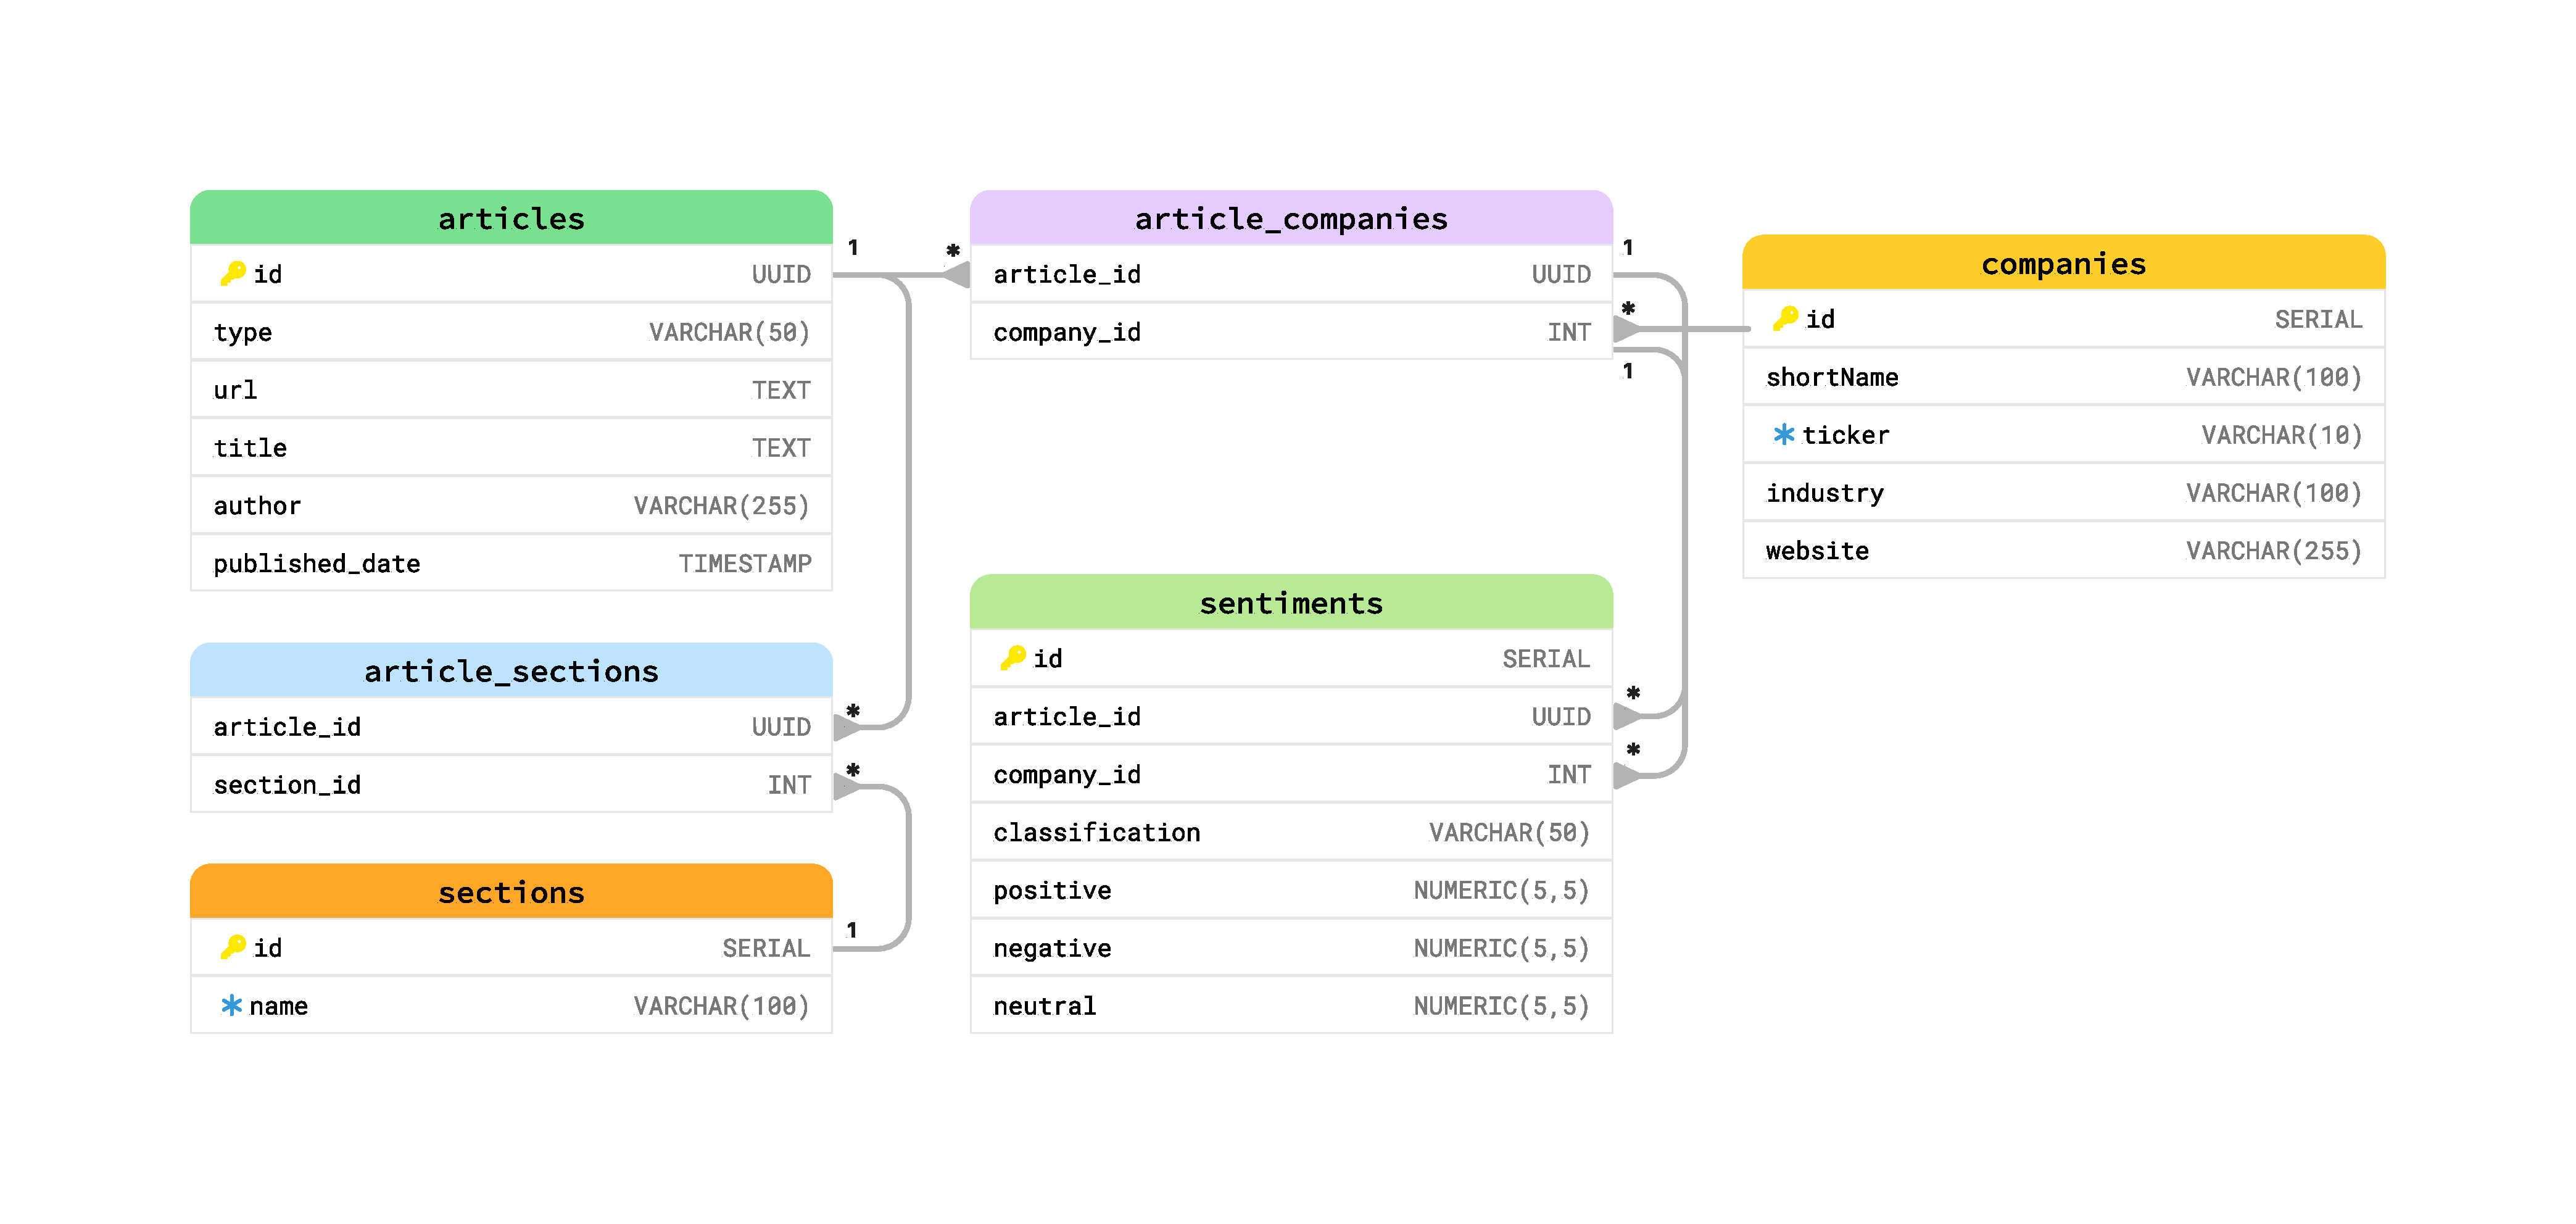
\includegraphics[width=\textwidth]{img/architecture/database-schema.pdf}
    \caption{Relational schema of \acrshort{etl} service database for storing article-related data.}
    \label{fig:architecture-etl-database-schema}
\end{figure}

Given the extensive utilisation of the join operation in our queries, we have established the three supplementary indexes on columns commonly employed for table joins. The following indexes are designed to improve the performance of queries that join data from these tables and respond to frequent queries more efficiently:

\begin{itemize}
    \item \textbf{\textit{idx\textunderscore article\textunderscore companies\textunderscore article\textunderscore id\textunderscore company\textunderscore id}} for columns \textit{article\textunderscore id} and \textit{company\textunderscore id} on the \textit{article\textunderscore companies} table
    \item \textbf{\textit{idx\textunderscore sentiments\textunderscore article\textunderscore id\textunderscore company\textunderscore id}} on the sentiments table for columns \textit{article\textunderscore id} and \textit{company\textunderscore id}
    \item \textbf{\textit{idx\textunderscore article\textunderscore sections\textunderscore article\textunderscore id\textunderscore section\textunderscore id}} on the \textit{article\textunderscore sections} table for columns \textit{article\textunderscore id} and \textit{section\textunderscore id}
\end{itemize}

Suppose we would like to incorporate more types of entities into the database in the future, such as people, events, or products with various relationships between them. In that case, we might consider using a graph database like Neo4j. Nevertheless, the relational model in the current stage of the application version is the most suitable choice for storing current type of data.

\subsubsection{Extract Details}
\label{subsubsec:architecture-etl-extract-details}
During implementation, we focused on making connecting additional sources for extraction effortless. Currently, we use only one source, the Guardian, for reasons outlined in Chapter \ref{chap:textual-data}. If we wanted to add more sources, it would be cautious to discuss and consider a filter to determine how similar articles from different sources are to avoid duplicating sentiment values from articles with the same content. Alternatively, we could account for this information in another way, such as weighting the sentiment based on the source's popularity and potential reach, which could impact the market.

Each source creates a separate tasks pipeline in Airflow within a single \acrshort{dag}, containing all phases of the \acrshort{etl} process. This approach allows us to easily add new sources without modifying the existing pipeline. The phases are divided into tasks and task groups, ensuring clarity, comfortable navigation in the code, simple implementation, and the possibility of parallel execution of individual tasks.

Specifically, extraction is performed as a single task for the Guardian source by requesting the Open Platform. The time frame for extracting articles is set to three months. During this period, about $1000$ articles is extracted, focusing on the business and technology sections. The endpoint paginates data in batches of $200$ articles. After determining the number of pages, a task is created for each page to retrieve the data and save it to a file. This method was chosen because the API limits the number of articles we can retrieve simultaneously, making pagination necessary. On the other hand, we can use this guideline to clearly define the data size distribution for individual tasks. Thus, it allows us to monitor the extraction process and ensure parallel execution in the subsequent transform phase.

\subsubsection{Transform Details}
\label{subsubsec:architecture-etl-transform-details}
The transform phase begins by reading the extracted data stored in files. It simplifies storing the final transformed data without copying and updating existing files. This ensures the data is available even if an error occurs in the subsequent phases and allows for continuous monitoring. Airflow provides cross-communication (X-Coms) data, which is loaded into metadata and can be easily passed between tasks. Although we know about the limitations, it is generally not recommended to transfer extensive data (approximately $1$ GB) using X-Com with a Postgres database supporting Airflow \parencite{laura2023-medium}. In our case, individual files of $200$ articles with file sizes ranging from $1$ to $2$ MB, making it acceptable with a substantial reserve.

The \acrshort{ner} task pulls article content data from X-Coms and sends the content to the \acrshort{ner} service \acrshort{api} endpoint. The response contains entities, each with its ticker and the substring defining the entity in the text. The result is then pushed into X-Coms as separate data. It ensures that the \acrshort{ner} task results are available for the subsequent \acrshort{sa} task.

The \acrshort{sa} task pulls article content and entity data from X-Coms. It sends the content and identified entities to the \acrshort{sa} service API endpoint, which responds with sentiments for each entity. The results are then pushed into X-Coms as another data collection containing entities and their sentiments for each article.

The results from X-Coms are combined with the original article data from the extract phase, excluding the content that no longer needs to be stored. The combined results are saved into files used in the subsequent load phase. This approach ensures a transparent and efficient processing workflow, which can be defined in task groups containing individual task dependencies, allowing for parallel data processing (see Figure \ref{fig:architecture-etl-transform}).

\begin{figure}[htbp]
    \centering
    \includegraphics[width=\textwidth]{img/architecture/etl-transform.pdf}
    \caption{The transform phase task groups and its tasks in the \acrshort{dag} of Guardian's \acrshort{etl} process. Directed from left to right.}
    \label{fig:architecture-etl-transform}
\end{figure}

\subsubsection{Load Details}
\label{subsubsec:architecture-etl-load-details}
The load phase begins with sequentially transformed data bulk loading into the database. In the current version, we do not employ loading in parallel because we have found that the approximate load duration time (see Table \ref{fig:architecture-etl-load}), in addition to a slowdown due to extra indexes, is acceptable, and parallel loading is unnecessary. It could lead to collisions where multiple sources simultaneously write to the same table. This approach could compromise data integrity and lead to database errors, especially when articles containing the same entities are inserted into the table concurrently. While row locking could mitigate this issue, it would slow down the entire process and increase system complexity, which could be counterproductive given the current data volume. Therefore, we prefer sequential data loading from a single source. The entire process of the Load phase is illustrated in Figure \ref{fig:architecture-etl-load}.

After loading data from individual task groups of sections, there is a task to insert additional company data into the database. This task involves inserting previously mentioned data such as short name, industry, and website from Yahoo Finance. Subsequently, there is a task that removes articles that do not contain any tickers. These articles are unusable to us, and their removal helps maintain data cleanliness in the database and reduces unnecessary database load.

\begin{table}[ht]
    \centering
    \caption{The approximate duration of individual tasks and task groups in the \acrshort{etl} process for the Guardian source.}
    \label{table:etl-task-durations}
    \begin{tabular}{l c}
        \hline
        \textbf{Task \& Task Group} & \textbf{Duration [min]} \\
        \hline
        replicated\_and\_clear\_tables & 0.02 \\
        insert\_additional\_data & 0.98 \\
        delete\_articles\_without\_companie & 0.02 \\
        delete\_replicated\_tables & 0.02 \\
        \hline
        \textbf{extract\_the\_guardian\_data} & 0.09 \\
        \hline
        \textbf{transform\_the\_guardian\_data} & 44 \\
        \hline
        transform\_business & 42 \\
        transform\_technology & 44 \\
        \hline
        \textbf{load\_the\_guardian\_data} & 0.35 \\
        \hline
        load\_technology & 0.08 \\
        load\_business & 0.22 \\
        \hline
    \end{tabular}
\end{table}

\begin{figure}[ht]
    \centering
    \includegraphics[width=\textwidth]{img/architecture/etl-load.pdf}
    \caption{The load phase task groups and its tasks in the \acrshort{dag} of Guardian's \acrshort{etl} process. Directed from left to right.}
    \label{fig:architecture-etl-load}
\end{figure}

According to Tabel \ref{table:etl-task-durations}, the transformation of the technology section, even though it contains only two pages (files) of articles, is completed in a similar time as the business section, which is twice as extensive. This is due to the distribution of jobs among workers, of which we have $16$ in our setup. The entire \acrshort{dag} work is automatically divided among the workers. However, the transformation results primarily depend on the response times of the \acrshort{ner} and \acrshort{sa} services. The \acrshort{sa} service, in particular, slows down the process owing to the computationally intensive FinABSA-Longer model, which has limited speed due to article content length. The average duration of \acrshort{ner} task groups is approximately $4$ minutes, while the average duration of \acrshort{sa} task groups\footnote{\acrshort{ner} task group in one task instance processes all 200 articles, whereas \acrshort{sa} processes only those that contain a ticker after NER is finished.} is $33$. The total runtime for a single execution of the entire pipeline, from extraction to loading and removing temporary tables, is approximately $45$ minutes. In the following subsection, we will examine the construction of requested services. Lastly, we propose how the \acrshort{dag} distribution might look by adding two more sources, shown in Figure \ref{fig:architecture-etl-sources}.

\begin{figure}[ht]
    \centering
    \includegraphics[width=0.8\textwidth]{img/architecture/etl-sources.pdf}
    \caption{The \acrshort{dag} of \acrshort{etl} phases for multiple sources, including the Guardian, New York Times, and Financial Times.}
    \label{fig:architecture-etl-sources}
\end{figure}

As mentioned, the time frame for extracting articles is set to three months. During this period, the database in the technology and business sections typically contains approximately the number of records indicated in Table \ref{table:architecture-etl-database-records}.

\begin{table}[ht]
    \centering
    \caption{The approximate number of records in the database tables after three months of time frame extraction employs the Guardian as the source focusing on business and technology sections.}
    \label{table:architecture-etl-database-records}
    \begin{tabular}{l c}
        \hline
        \textbf{Table} & \textbf{Records} \\
        \hline
        \textit{articles}       & 543 \\ 
        \textit{companies}      & 180 \\ 
        \textit{sections}       & 2 \\
        \textit{sentiments}     & 1,327 \\
        \textit{article\textunderscore companies} & 1,327 \\
        \textit{article\textunderscore sections}  & 543 \\
        \hline
    \end{tabular}
\end{table}

\subsection{Named Entity Recognition Service}
\label{subsec:architecture-ner}
The \acrshort{ner} service categorises entities in article content data. Its core component is the named entity recognition algorithm, detailed in Chapter \ref{chap:comapny-to-symbol-linking}. We emphasise identifying organisation-type entities and filtering to determine companies\footnote{Reminder that organisations can be considered potential companies. An organisation is defined as a company if it has a ticker.} specifically within the algorithm. This service plays a crucial role in subsequent data processing, as the entities obtained serve as input for the \acrshort{sa} service.

This service operates as a FastAPI\footnote{\href{https://www.fastapi.tiangolo.com}{https://www.fastapi.tiangolo.com}} server, offering a POST request endpoint to extract entities from article content. The output includes a list of entities containing a ticker symbol and a substring representing the entity in the text. Especialy, \acrshort{sa} service then processes substring further in analysis. Upon requesting this endpoint, results are returned to the \acrshort{etl} process during its transformation phase before continuing to the \acrshort{sa} service. The following Figure \ref{fig:architecture-ner-req-res} shows the schema of a POST request to the \acrshort{ner} service for extracting entities from article content and its response.

\begin{figure}[ht]
    \centering
    \includegraphics[width=\textwidth]{img/architecture/ner-req-res.pdf}
    \caption{Schema of a POST request to the \acrshort{ner} service for extracting entities from article content and its response.}
    \label{fig:architecture-ner-req-res}
\end{figure}

The need for the fastest response times and efficient data handling drove the choice of the FastAPI framework. Its speed, user-friendly nature, and broad user community are the main reasons for its selection. It integrates seamlessly with the Pydantic library\footnote{\href{https://docs.pydantic.dev/}{https://docs.pydantic.dev/}}, allowing data to be defined as Python classes that automatically generate JSON schemas for data validation within the FastAPI framework. Moreover, FastAPI is built on the Asynchronous Server Gateway Interface\footnote{\href{https://asgi.readthedocs.io/en/}{https://asgi.readthedocs.io/en/}} (ASGI) framework, which is suitable for our querying of Wikidata. The asynchronous implementation of the code allows operations to run independently of the server's main thread, enabling the server to handle more requests and perform other tasks while waiting for a response or processing data retrieved from Wikidata. This is highly desirable for our \acrshort{etl} pipeline, where processing large amounts of data is necessary while maintaining processing speed. Due to the server's limitations on which the \acrshort{ner} service runs, the endpoint is handled by two workers for request processing.

\subsection{Sentiment Analysis Service}
\label{subsec:architecture-sa}
The \acrshort{sa} service analyses the sentiment of text at the entity level, classifying it as positive, negative, or neutral based on the highest sentiment score in one of these categories. The core component of this service is a sentiment analysis algorithm, which is detailed in Chapter \ref{chap:entity-level-sentiment-analysis}. This service is crucial for determining the sentiment of entities extracted from the article content by the \acrshort{ner} service.

This service operates, like the \acrshort{ner} service, as an independent FastAPI server, offering a post request endpoint to analyse the sentiment of entities. The output includes a sentiment score for all categories and a classification for each company in the text. The sentiment scores are a floating-point number between $0$ and $1$, and their sum is equal to $1$. The higher the score, the more the given category is expressed. Thus, sentiment for a given company has a structure that includes classification, positive, neutral, and negative values. The following Figure \ref{fig:architecture-sa-req-res} shows the schema of a post request to the \acrshort{sa} service for analysing the sentiment of entities in article content and its response.

\begin{figure}[ht]
    \centering
    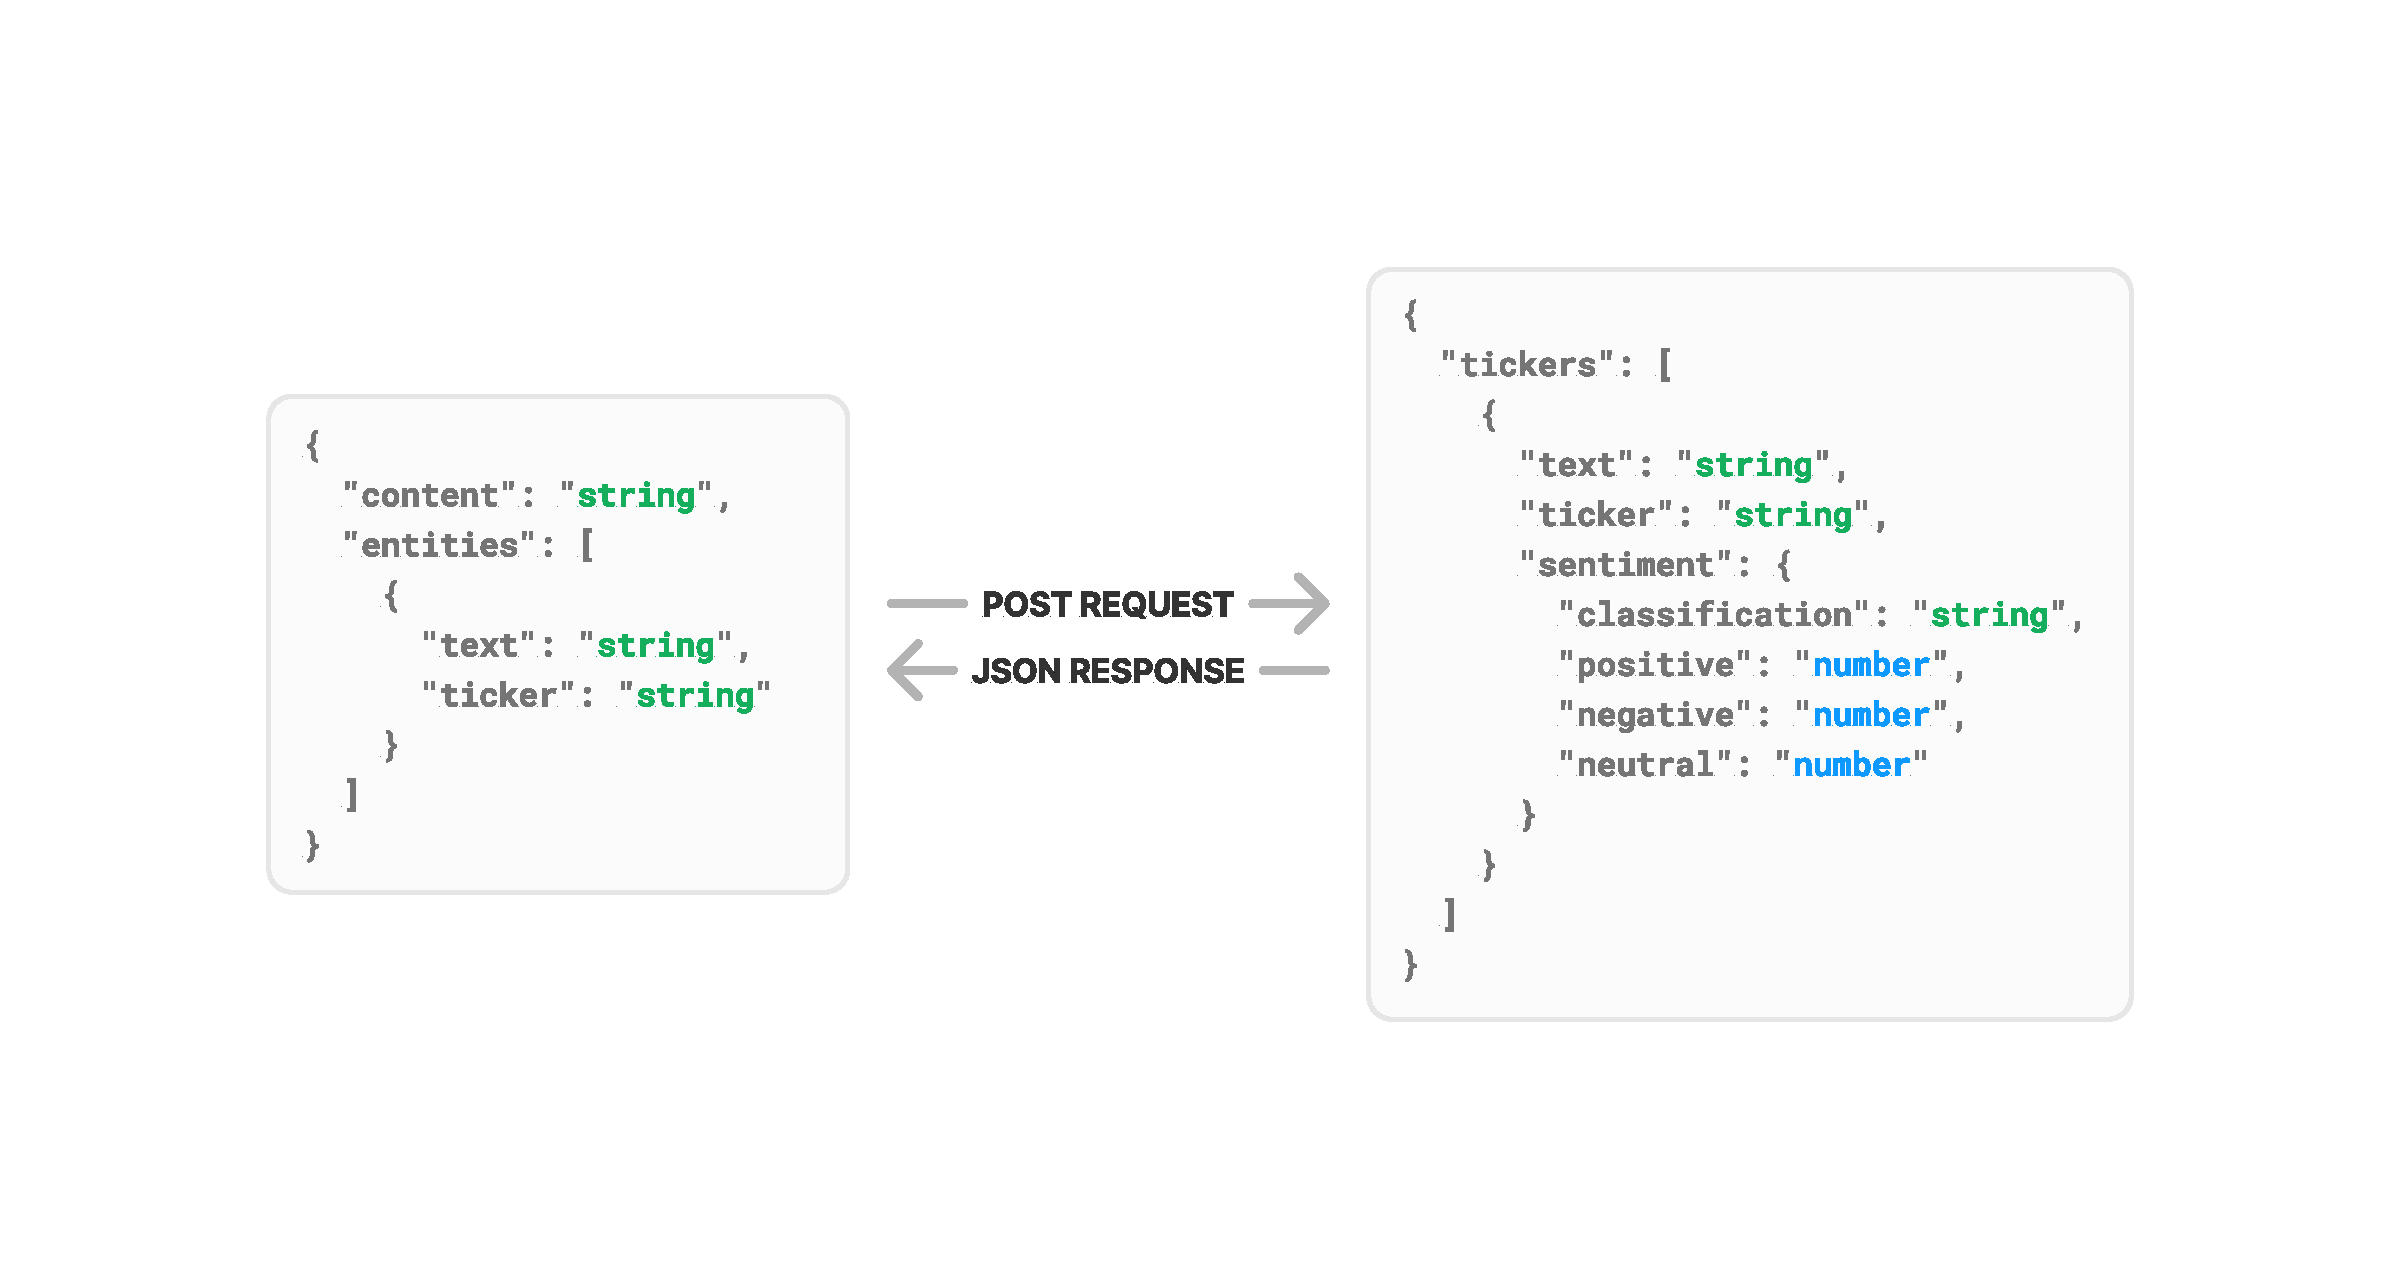
\includegraphics[width=\textwidth]{img/architecture/sa-req-res.pdf}
    \caption{Schema of a POST request to the SA service for sentiment analysis of extracted entities in article content and its reponse.}
    \label{fig:architecture-sa-req-res}
\end{figure}

Like the \acrshort{ner} service built on ASGI, the FastAPI framework was also selected for its speed and efficiency. Being built on ASGI enables FastAPI to be implemented asynchronously, which is beneficial for processing data from the \acrshort{ner} service. Despite sentiment analysis demanding more computational power, two workers also manage the endpoint. The interval we have set for repeating the \acrshort{dag} is $4$ hours, sufficient for processing speed, meaning processing takes $49$ minutes and repeats every $4$ hours.

\subsection{REST API Service}
\label{subsec:architecture-rest-api}
The \acrshort{restapi} service primarily provides access to data stored in the database. It is responsible for handling requests from the frontend and returning the appropriate data to be displayed to users. This service uses Flask\footnote{\href{https://www.flask.palletsprojects.com/en/3.0.x/}{https://www.flask.palletsprojects.com/en/3.0.x/}}, a lightweight Web Server Gateway Interface\footnote{\href{https://wsgi.readthedocs.io/en/}{https://wsgi.readthedocs.io/en/}} (WSGI) web application microframework. This framework is chosen for its flexibility, simplicity, and ease of extensibility. Most importantly, it provides more satisfactory control and management of schemas and resources than FastAPI, which is crucial for the purposes of this \acrshort{api}.

The \acrshort{api} handles the connection to the database using a controller, which grants access to all data from the \acrshort{etl} process. It scans whether temporary tables are available in the database during each request, which exists only during the \acrshort{etl} process. Furthermore, since the main tables are empty during \acrshort{etl}, it queries the replicated temporary tables. After the \acrshort{etl} process ends, these tables are removed, and the \acrshort{api} accesses the main tables containing data after the recent \acrshort{etl}. The \acrshort{api} is designed to handle frontend requests and provide responses with data in JSON format. Thus, the output is a JSON file containing data from the database, which is then displayed to users.

The \acrshort{api} provides the following endpoints, which we will not specify in detail with images like the previous two services but only summarise. We refer directly to the Swagger documentation, which we specify in more detail in Chapter \ref{chap:development-documentation}, for a detailed description of schemas and resources. Here is a summary of the endpoints, all of which are in the form of GET requests:

\begin{itemize}
    \item \textbf{Company Info} fetches a company's information from the database, as well as daily high and low prices and market volume from Yahoo Finance.
        \begin{itemize}
            \item \textit{/api/v0/company/\{ticker\}/info}
        \end{itemize}
    \item \textbf{Company Chart} fetches a company's chart data, such as sentiment, from the database and adjusted close price from Yahoo Finance to be displayed in chart.
        \begin{itemize}
            \item \textit{/api/v0/company/\{ticker\}/chart}
        \end{itemize}
    \item \textbf{Company Article List} fetches a company's articles from the database.
        \begin{itemize}
            \item \textit{/api/v0/company/\{ticker\}/articles}
        \end{itemize}
    \item \textbf{Company Graph} fetches a company's graph data from the database to be displayed as a graph network.
        \begin{itemize}
            \item \textit{/api/v0/company/\{ticker\}/graph}
        \end{itemize}
    \item \textbf{Companies Names and Tickers} fetches all companies' names and tickers from the database.
        \begin{itemize}
            \item \textit{/api/v0/companies/names}
        \end{itemize}
    \item \textbf{Companies Graphs} fetches all companies' graphs from the database to be displayed as a graph network.
        \begin{itemize}
            \item \textit{/api/v0/companies/graphs}
        \end{itemize}
\end{itemize}

\section{Frontend}
\label{sec:frontend}
The frontend is written using the Angular framework. Its principal function is to provide a user interface for interacting with data from the database through a \acrshort{restapi}. In our case, it communicates solely with the backend \acrshort{restapi} to retrieve and display data without making any updates. Built on top of TypeScript, Angular adds static typing and other features that simplify the development and implementation of the code. It offers many features, such as a modular architecture, which makes it easy to split an application into smaller parts, including components, services, and routing.

Although Angular is a frontend framework, infrastructure such as Docker or other server software is required to run it on a server. This infrastructure is used to deploy and serve the frontend application to users. Deploying an Angular application requires a server that provides users with static files. It is also built for single-page applications, which is an ideal solution in our case because the application can be more efficient, easily scalable, and maintainable, which is essential for long-term development. As part of the architecture and communication with other services, we create models in the form of interfaces that can be directly mapped to individual endpoints in the \acrshort{restapi}, which we can query its endpoints through an HTTP service.

The most significant benefit of Angular is its component architecture. The cornerstone is the component, composed of a TypeScript class, an HTML template, and styles typically in CSS. Components are reusable and can be easily moved to other application parts. This makes deploying new components smooth and effortless, increasing development efficiency. The flowchart navigation of application pages is illustrated in Figure \ref{fig:architecture-frontend-flowchart} below for a better understanding of the frontend structure. The following subsections describe each application component.

\begin{figure}[ht]
    \centering
    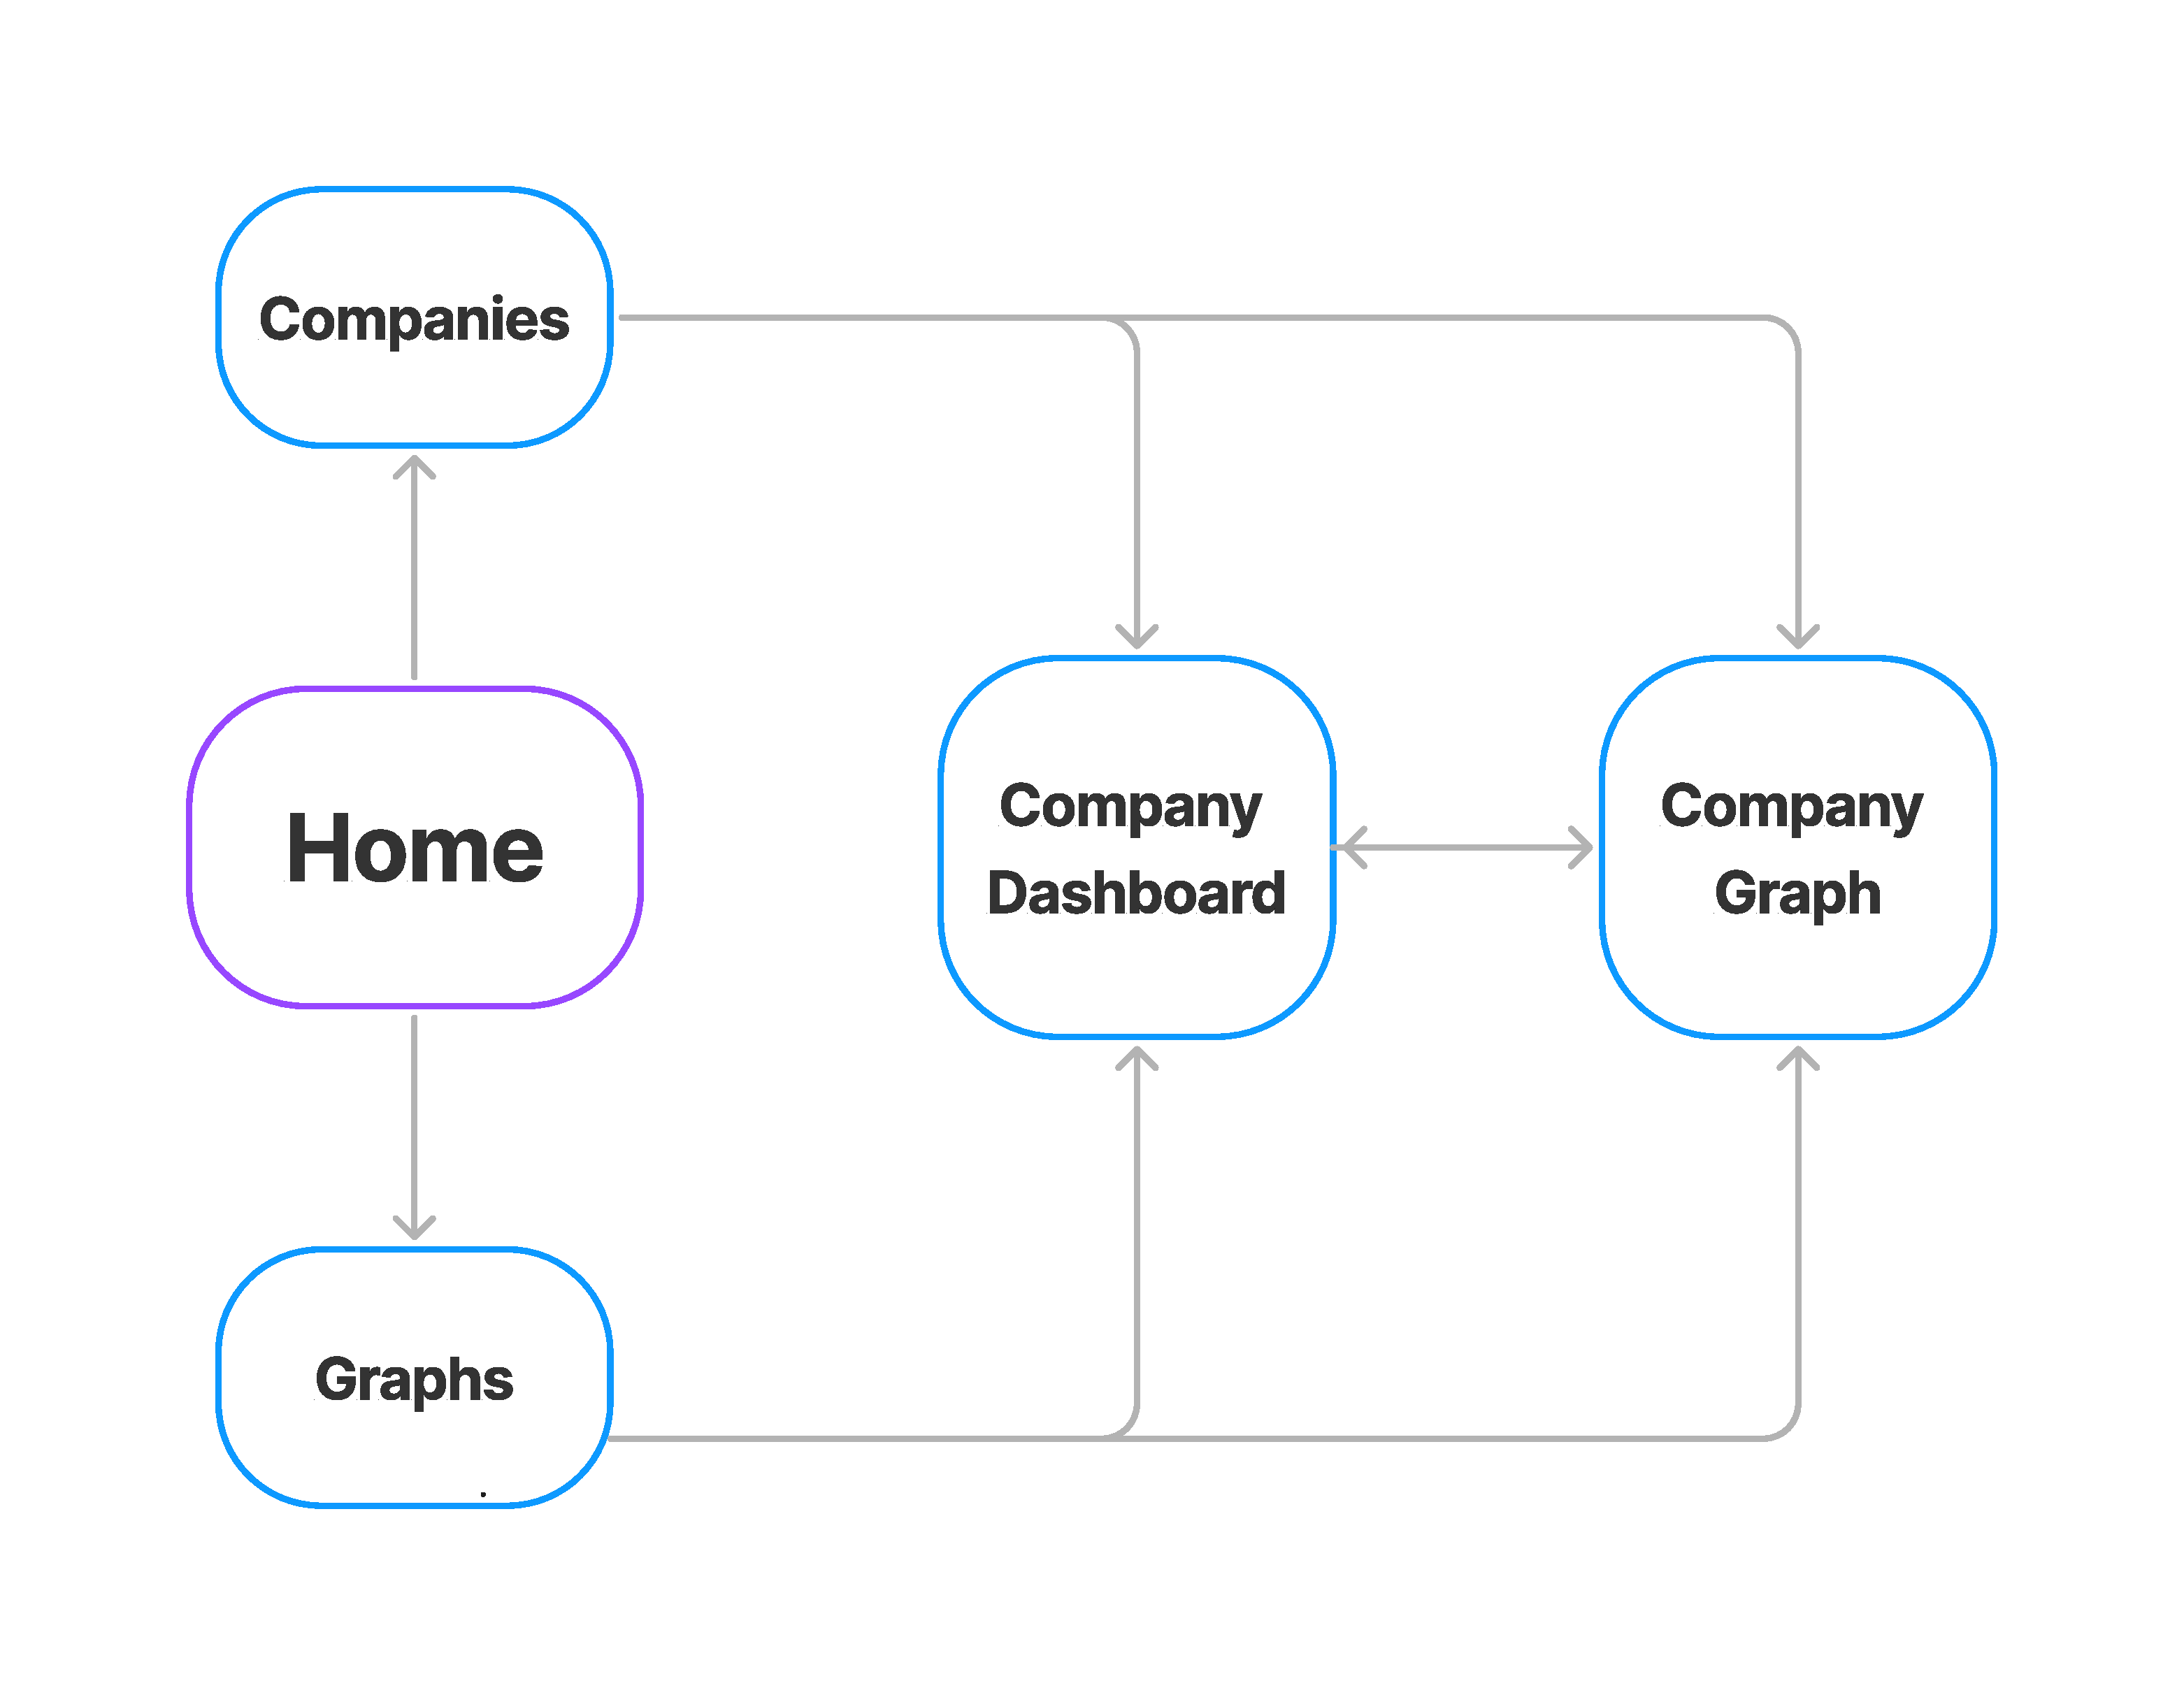
\includegraphics[width=0.7\textwidth]{img/architecture/website-flowchart.pdf}
    \caption{Flowchart navigation of application pages in the frontend.}
    \label{fig:architecture-frontend-flowchart}
\end{figure}

\subsection{Home Component}
\label{subsec:frontend-home}
This component serves as the homepage and does not contain any other components. It only displays an introduction describing the application. It includes a navigation bar, allowing users to access other application pages, such as graphs or companies.

\subsection{Graphs Component}
\label{subsec:frontend-graphs}
This component represents a page that displays the connections between individual articles and companies. The 3D Force Graph library, available on GitHub\footnote{\href{https://www.github.com/vasturiano/3d-force-graph}{https://www.github.com/vasturiano/3d-force-graph}}, provides the graph visualisation web component based on ThreeJS\footnote{\href{https://www.github.com/mrdoob/three.js/}{https://www.github.com/mrdoob/three.js/}}/WebGL for 3D rendering and d3-force-3d\footnote{\href{https://www.github.com/vasturiano/d3-force-3d}{https://www.github.com/vasturiano/d3-force-3d}} or ngraph\footnote{\href{https://www.github.com/anvaka/ngraph.forcelayout3d}{https://www.github.com/anvaka/ngraph.forcelayout3d}} for the core physics engine. An edge links an article to a company if the company is mentioned in the article. The edge colour represents the sentiment towards the company in the article. The colour of the articles varies based on their average sentiment towards all mentioned companies, while the company's colour is blue to distinguish it from the articles. Additionally, the edge colour indicates the sentiment associated with the specific company. 

The graph can be navigated and displayed, with control panels included for manipulating and modifying the graph visualisation. Users can filter the graph based on the average sentiment of individual articles and adjust the graph size to modify the visualisation. Each article can be viewed on the Guardian or navigated to the company graph or dashboard. The higher the mentioned companies within the article, the higher the article node size. The same applies to the company node. The higher mentioned in articles, the higher the company node size. We can smoothly identify the most trending companies in the articles. The interactive graph allows users to zoom in and out, rotate, and drag nodes. Additionally, graph traversal simulating the visibility of only neighbouring vertices is also implemented. The graph is loaded from the \acrshort{restapi} companies graphs endpoint.

\subsection{Companies Component}
\label{subsec:frontend-companies}
This component represents a page for searching individual companies' dashboards or graphs. It allows users to search for companies by name or ticker, implemented through Angular's ngx-pipes for efficient data manipulation and sorting by default. After searching, navigating to the selected company's dashboard or company graph component is possible. Like the home component, it also includes a navigation bar from which users can navigate to the graphs or home page. Data are loaded from the \acrshort{restapi} companies names and tickers enpoint.

\subsection{CompanyGraph Component}
\label{subsec:frontend-graph}
This component serves as a page, similar to the graphs component, but offers a slightly different view of the connections between individual articles and a specific company. The purpose is to reflect sentiment only to the individual company. Colouring in the graph works the same way as before. However, in this case, the article's node colours are based solely on the sentiment towards the specific company and not on the average sentiment of all the companies mentioned. Additionally, it contains control panels similar to those of the graph component. The graph is loaded from the \acrshort{restapi} company graph endpoint.

\subsection{CompanyDashboard Component}
\label{subsec:frontend-dashboard}
This component acts as a parent component to load individual child components. As the parent component, it loads data and then passes it to its children through the input decorator. This way, all data transfer is handled in one component, which then distributes it for loading. The child components of the company dashboard are as follows:

\begin{itemize}
    \item \textbf{CompanyInfo Component}: Displays brief information about the company.
    \item \textbf{Charts}: Individual charts are created using the CanvasJS\footnote{\href{https://www.canvasjs.com}{https://www.canvasjs.com}} library, which provides simple and efficient implementation within the Angular framework. Data for the charts is loaded from the \acrshort{restapi} company chart endpoint. The following charts are included:
    \begin{itemize}
        \item \textbf{StockChart Component}: Displays sentiment and adjusted close price in a stock chart average seniment for each day.
        \item \textbf{PieChart Component}: Shows the distribution of average sentiment over time in a pie chart.
        \item \textbf{SplineChart Component}: Illustrates each category of sentiment over time in a spline chart. 
    \end{itemize}
    \item \textbf{ArticleList Component}: Lists all articles mentioning the company, including relevant data such as title, date, link to the article, author, section, and sentiment. Data can be sorted and searched using text that applies to data in the table across all attributes. The listing is implemented through the material paginator provided by Angular. Data are loaded from the \acrshort{restapi} company article list endpoint.
\end{itemize}

By utilising the input decorator, data for all three charts is loaded only once, allowing us to clearly and efficiently create at least three charts without loading data separately for each chart. Additionally, data loaded into the CompanyInfo and ArticleList components come from specific endpoints explicitly created for their purpose. This approach allows us to effortlessly and efficiently implement additional components we want to include in the dashboard in the future.
\chapter{Development Documentation}
\label{chap:development-documentation}
Since the algorithms and the concepts of named entity recognition and sentiment analysis applied to each service have been thoroughly described in Chapters \ref{chap:comapny-to-symbol-linking}, \ref{chap:entity-level-sentiment-analysis}, and the architecture in Chapter \ref{chap:architecture}, this chapter will only briefly summarize the essential points. For more detailed information, we will refer to the documentations produced by pdoc\footnote{\href{https://pdoc3.github.io/pdoc/}{https://pdoc3.github.io/pdoc/}}. This documentation includes extensive functional and module comments and adheres to the PEP8\footnote{\href{https://peps.python.org/pep-0008/}{https://peps.python.org/pep-0008/}} standard. Additionally, Chapter \ref{chap:architecture} thoroughly describes the \acrshort{etl} process, covering the various steps required to obtain and prepare the data for subsequent analysis. The frontend documentation has not been generated, so we will discuss it in more depth. However, it also contains strong enough comments to describe the functionality.

Our deployment details are not included in this text because the application is available on a server provided by the university. Unified services run on the server, each handled by Docker to ensure independent functionality. Only two server ports are tunnelled, as we only need one to manage \acrshort{etl} service through the Airflow webserver and one to provide access to the frontend. The \acrshort{api} services have their OpenAPI specifications in JSON generated by Swagger\footnote{\href{https://swagger.io}{https://swagger.io}}, which can be displayed within Swagger EDITOR\footnote{\href{https://editor.swagger.io}{https://editor.swagger.io}}.

\section{Backend}
\label{sec:development-backend}

\subsection{Extract Transform Load Service}
\label{subsec:development-etl}
The extract transform load service is located in the directory \textit{/app/backend/extract-transform-load}.

\begin{itemize}
    \item \textbf{Documentation}: \textit{/docs/documentation/dev/etl}.
    \item \textbf{Airflow Webserver} is availible on server\footnote{Contact me for more information.}, use Viewer account 
    \begin{itemize}
        \item \textbf{login}: \textit{viewer}
        \item \textbf{password}: \textit{viewer}
    \end{itemize}
    \item \textbf{Main Directories}
    \begin{itemize}
        \item \textbf{\textit{/airflow}} - contains the Airflow \acrshort{dag} loading script to the Airflow and the configuration files
        \item \textbf{\textit{/dag}} - contains the \acrshort{etl}'s \acrshort{dag}, detailed in attached documentation
        \item \textbf{\textit{/data}} - contains the \acrshort{etl} phases data checkpoints
        \item \textbf{\textit{/scripts}} - contains Docker scripts for the Airflow and Postgres initialisation.
    \end{itemize}
\end{itemize}

\subsection{Named Entity Recognition Service}
\label{subsec:development-ner}
The named entity recognition service is located in the directory \textit{/app/backend/named}\textit{entity-recognition}.

\begin{itemize}
    \item \textbf{Documentation}: \textit{/docs/documentation/dev/ner}.
    \begin{itemize}
        \item \textbf{OpenAPI}: \textit{openapi.json}
    \end{itemize}
    \item \textbf{Main Directories} are detailed described in the documentation.
    \item \textbf{Spacy Model}: \textit{en\_core\_web\_md}
    \item \textbf{Spacy Entity Linker Model}: version $1.0.3$
\end{itemize}

\subsection{Sentiment Analysis Service}
\label{subsec:development-sentiment}
The sentiment analysis service is located in the directory \textit{/app/backend/sentiment-analysis}.

\begin{itemize}
    \item \textbf{Documentation}: \textit{/docs/documentation/dev/sentiment}.
    \begin{itemize}
        \item \textbf{OpenAPI}: \textit{openapi.json}
    \end{itemize}
    \item \textbf{Main Directories} are detailed described in the documentation.
    \item \textbf{Analysis Model}: \textit{amphora/FinABSA-Longer}
\end{itemize}

\section{REST API Service}
\label{sec:development-rest-api}
The \acrshort{restapi} service is located in the directory \textit{/app/backend/rest-api}.

\begin{itemize}
    \item \textbf{Documentation}: \textit{/docs/documentation/dev/rest-api}.
    \begin{itemize}
        \item \textbf{OpenAPI}: \textit{openapi.json}
    \end{itemize}
    \item \textbf{Main Directories} are described in the documentation, within resources and schemata, and in OpenAPI documentation.
    \item \
\end{itemize}

\section{Frontend}
\label{sec:development-frontend}
The frontend service is located in the directory \textit{/app/frontend}. The frontend components are structured in the following way:

\subsection{Components Overview}
\label{subsec:development-components-overview}
The frontend components are structured in the following way:

\subsubsection{HomeComponent}
\label{subsubsec:development-home}
The \textit{HomeComponent} is a simple component with no data mapping. It is dedicated to displaying the home page.

\subsubsection{CompaniesComponent}
\label{subsubsec:development-companies}
The \textit{CompaniesComponent} is dedicated to searching for companies using the \textit{CompanyName} model as a list, which is directly mapped to data from the \acrshort{restapi} endpoint \textit{/api/v0/companies/names}.

\subsubsection{DashboardComponent}
\label{subsubsec:development-dashboard}
The \textit{DashboardComponent} is a parent component fetching data for its child components. While data are fetching for each child component separately, the data loading bar is displayed within the separate children. The child components are as follows:

\begin{itemize}
    \item \textbf{ArticleListComponent} - component dedicated to displaying all articles as a list. It is directly mapped to data from the \acrshort{restapi} endpoint \textit{/api/v0/company/}-\textit{\{ticker\}/articles} using the \textit{CompanyArticlesList} model.
    
    \item \textbf{CompanyInfoComponent} - component dedicated to displaying company information. It is directly mapped to data from the REST:
    \begin{itemize}
        \item \textbf{Endpoint}: \textit{/api/v0/company/\{ticker\}/info}  
        \item \textbf{Model}: \textit{CompanyInfo}
    \end{itemize}
    
    \item \textbf{PieChartComponent} - component dedicated to displaying the company's daily average sentiment value distribution in a pie chart. It is directly mapped to data from the \acrshort{restapi} :
    
    \begin{itemize}
        \item \textbf{Endpoint}: \textit{/api/v0/company/ticker/chart}  
        \item \textbf{Model}: \textit{CompanyChart}
    \end{itemize}
    
    \item \textbf{SplineChartComponent} - component displaying company sentiment value evolution in a spline chart. It is directly mapped to data from the \acrshort{restapi}:
    \begin{itemize}
        \item \textbf{Endpoint}: \textit{/api/v0/company/\{ticker\}/chart}  
        \item \textbf{Model}: \textit{CompanyChart}
    \end{itemize}

    \item \textbf{StockChartComponent} - component dedicated to displaying company price and sentiment. It is directly mapped to data from the \acrshort{restapi}:
    \begin{itemize}
        \item \textbf{Endpoint}: \textit{/api/v0/company/\{ticker\}/chart}  
        \item \textbf{Model}: \textit{CompanyChart}
    \end{itemize}
\end{itemize}

\subsubsection{GraphsComponent}
\label{subsubsec:development-graphs}
The \textit{GraphsComponent} is a component dedicated to displaying all companies and articles as one graph. The components are separated into \textit{Graph} and \textit{Graphs} due to the ability to customise the graph and display the data so that the user can easily understand the data. It is directly mapped to data from the \acrshort{restapi}:

\begin{itemize}
    \item \textbf{Endpoint}: \textit{/api/v0/companies/graphs}
    \item \textbf{Model}: \textit{CompaniesGraphs}
\end{itemize}

\subsection{Services Overview}
\label{subsec:development-services-overview}
The frontend services provide communication with the \acrshort{restapi}. Using the \textit{HttpClient} module requesting GET methods to the endpoints using dedicated models to ensure data consistency.

\subsection{Routes}
\label{subsec:development-routes}
The frontend routes manage navigation through the application. It uses the \textit{RouterModule} to navigate between components. If \textit{ticker} is in the URL, the application will automatically load the company data related to the company with the given \textit{ticker}.

\begin{itemize}
    \item \textbf{HomeComponent}: \textit{/} or \textit{/home}
    \item \textbf{CompaniesComponent}: \textit{/companies}
    \item \textbf{GraphsComponent}: \textit{/companies/graphs}
    \item \textbf{GraphComponent}: \textit{/company/:ticker/graph}
    \item \textbf{DashboardComponent}: \textit{/company/:tickerdashboard}
\end{itemize}


\chapter{User Documentation}
\label{chap:user-documentation}

\section{Home}
\label{sec:user-documentation-home}
The home page is the initial page the users see after visiting the website (see Figure \ref{fig:user-documentation-home}). Users can navigate to the graphs page, which presents a comprehensive network of articles spanning the last three months. Additionally, they have access to the companies page, which provides a detailed listing of companies.

\begin{figure}[ht]
  \centering
  \includegraphics[width=\textwidth]{img/user/home-a.pdf}
  \caption{The website's home page briefly describing the project and its purpose.}
  \label{fig:user-documentation-home}
\end{figure}

\section{Graphs}
\label{sec:user-documentation-graphs}
The graphs page displays a network of all articles from the past three months. Each edge represents the sentiment of the company mentioned in the article, indicated by its colour. The article node's colour represents the average sentiment of all connected companies. Hovering over a node reveals its name if it is a company or its title if it is an article (see Figure \ref{fig:user-documentation-graphs}). Furthermore, neighbouring nodes are highlighted.

\begin{figure}[ht]
    \centering
    \includegraphics[width=\textwidth]{img/user/graphs-a.pdf}
    \caption{Users can see the network of all articles for the past three months by navigating to the graphs page.}
    \label{fig:user-documentation-graphs}
\end{figure}

\subsection{Control Panels}
\label{subsec:control-panel}
The control panels on the upper right side of the page are categorized into two types. The first type is the general control panel, specifically designed for managing the network graphs and encompasses the following features:
\begin{itemize}
    \item \textbf{Distances}
    \begin{itemize}
        \item \textbf{Positive distance} - regulates the distance of the edge with positive sentiment.
        \item \textbf{Neutral distance} - regulates the distance of the edge with neutral sentiment.
        \item \textbf{Negative distance} - regulates the distance of the edge with negative sentiment (see Figure \ref{fig:user-documentation-graphs-distances}). 
    \end{itemize}
    \item \textbf{Visibility}\footnote{Visibility filtering is not available when only neighbouring nodes are visible. Refer to its corresponding company graph page for specific node examination and filtering.}
    \begin{itemize}
        \item \textbf{Show only negative sentiment} - shows only the article nodes with negative sentiment (see Figure \ref{fig:user-documentation-graphs-only-negative}).
        \item \textbf{Show only neutral sentiment} - shows only the article nodes with neutral sentiment.
        \item \textbf{Show only positive sentiment} - shows only the article nodes with positive sentiment.
    \end{itemize}
\end{itemize}

Another control panel is available for node details, which appears upon left-clicking on an article node. It provides the following options:

\begin{itemize}
    \item \textbf{Article node}
    \begin{itemize}
        \item \textbf{Title} - the title of the article.
        \item \textbf{Published date} - the date when the article was published.
        \item \textbf{Author} - the author of the article.
        \item \textbf{Open article} - the link to the article.
        \item \textbf{Average sentiment} - the average sentiment of the article is based on the average sentiment of the companies mentioned.
        \item \textbf{Companies} - the list of companies mentioned in the article with their sentiment. It expands on details about the company and its sentiment in the article (see Figure \ref{fig:user-documentation-graphs-article}).
    \end{itemize}
    \item \textbf{Company node}
    \begin{itemize}
        \item \textbf{Company information} - the details about the company, such as ticker and link to the company's dashboard or graph page.
        \item \textbf{Articles} - the list of articles in which the company is mentioned with the sentiment of the company in the article (see Figure \ref{fig:user-documentation-graphs-apple-negative}).
    \end{itemize}
\end{itemize}

\subsection{Actions}
\label{subsec:actions}
\begin{itemize}
    \item \textbf{Left click} on a node involves zoom-in, then it will show only the neighbours of the clicked node.
    \item \textbf{Right click} on a node will show all nodes back.
    \item \textbf{Hover node} shows a name of the company or the title of the article and highlights the neighbours.
\end{itemize}

\begin{figure}[htbp]
    \centering
    \includegraphics[width=\textwidth]{img/user/graphs-distances-a.pdf}
    \caption{The control panel managing edge distances. This involves selecting edges with sentiments and regulating them with values ranging from 100 to 3000. The image shows the network with the edge distances set to 100.}
    \label{fig:user-documentation-graphs-distances}
\end{figure}

\begin{figure}[htbp]
    \centering
    \includegraphics[width=\textwidth]{img/user/graphs-only-negative-a.pdf}
    \caption{After right-clicking, all nodes will be displayed back. The neutral and positive sentiments of the article nodes were turned off through the control panel. If there is an edge to the article node, then it remains to be visible.}
    \label{fig:user-documentation-graphs-only-negative}
\end{figure}

\begin{figure}[htbp]
    \centering
    \includegraphics[width=\textwidth]{img/user/graphs-article-a.pdf}
    \caption{After left-clicking on an article node, the control panel could be expanded with further information, such as listing all companies mentioned in the article with their sentiment as well as the average sentiment of the article and more detailed information about the title, date, author, and link to the article.}
    \label{fig:user-documentation-graphs-article}
\end{figure}

\begin{figure}[htbp]
    \centering
    \includegraphics[width=\textwidth]{img/user/graphs-apple-negative-a.pdf}
    \caption{Apple Inc. node with its neighbours after left click. The list of articles in which it is mentioned additionally provides the values of its sentiment, which is Apple's sentiment in that article. The article's colour indicates a negative average sentiment.}
    \label{fig:user-documentation-graphs-apple-negative}
\end{figure}

\newpage

\section{Companies}
\label{sec:user-documentation-companies}
The companies page allows the users to search for a company by its name or stock symbol. The users can also navigate to the company's dashboard or graph page (see Figure \ref{fig:user-documentation-companies-search}).

\begin{figure}[htbp]
    \centering
    \includegraphics[width=\textwidth]{img/user/search-am-a.pdf}
    \caption{Companies search allows the users to search for a company by its name or stock symbol. The image shows the search for ``am''.}
    \label{fig:user-documentation-companies-search}
\end{figure}

\newpage

\section{Company Dashboard}
\label{sec:user-documentation-company-dashboard}
The company dashboard offers users comprehensive information about the company through multiple components (see Figure \ref{fig:comapny-apple}).

\begin{figure}[htbp]
    \centering
    \includegraphics[width=\textwidth]{img/user/company-apple-a.pdf}
    \caption{Apple Inc. dashboard overview.}
    \label{fig:comapny-apple}
\end{figure}

\subsection{Company Information}
\label{subsec:company-information}
The company information component includes the company's name, stock symbol, and a graph link. It provides average daily sentiment values categorised as positive, neutral, or negative, updated every $4$ hours. Additionally, it displays Yahoo Finance data, including daily high, low, and volume, which is refreshed with each visit (see Figure \ref{fig:apple-info}).

\begin{figure}[htbp]
    \centering
    \includegraphics[width=\textwidth]{img/user/apple-info-a.pdf}
    \caption{Apple Inc. company information.}
    \label{fig:apple-info}
\end{figure}

\subsection{Stock Chart}
\label{subsec:stock-chart}
The stock chart component shows the adjusted close price of the company for the past three months. The users can zoom in and out by selecting the time range (see Figure \ref{fig:apple-stock}). The chart is divided into two parts; the upper part shows the price, and the lower part shows the daily average value of the company's sentiments in the articles for a given day.

Sentiments in the second part can be hidden by clicking on the sentiment legend. Hovering over the chart shows the date, stock price, and sentiment value for a given day (see Figure \ref{fig:apple-stock-range-neutral}).

\begin{figure}[htbp]
    \centering
    \includegraphics[width=\textwidth]{img/user/apple-stock-a.pdf}
    \caption{Apple Inc. stock chart in default view.}
    \label{fig:apple-stock}
\end{figure}

\begin{figure}[htbp]
    \centering
    \includegraphics[width=\textwidth]{img/user/apple-stock-range-neutral-a.pdf}
    \caption{Apple Inc. stock chart in two months range with hidden sentiment values except neutral (lean negative).}
    \label{fig:apple-stock-range-neutral}
\end{figure}


\subsection{Spline Chart}
\label{subsec:spline-chart}
The spline chart component demonstrates the evolution of the daily average sentiment value over the past three months. Users can hide the sentiment spline like in the stock chart by clicking on the sentiment legend. Hovering over the chart shows a given day's date and sentiment value (see Figure \ref{fig:apple-stock-spline}).

\begin{figure}[htbp]
    \centering
    \includegraphics[width=\textwidth]{img/user/apple-spline-chart-a.pdf}
    \caption{Apple Inc. spline chart displaying the daily average sentiment value evolution for the past three months.}
    \label{fig:apple-stock-spline}
\end{figure}

\subsection{Pie Chart}
\label{subsec:pie-chart}
The pie chart component illustrates the daily average sentiment values distribution for the past three months (see Figure \ref{fig:apple-pie}).

\begin{figure}[htbp]
    \centering
    \includegraphics[width=0.8\textwidth]{img/user/apple-pie-chart-a.pdf}
    \caption{Apple Inc. pie chart showing the daily average sentiment values distribution for the past three months.}
    \label{fig:apple-pie}
\end{figure}

\subsection{Article List}
\label{subsec:article-list}
The article list component shows the list of articles in which the company is mentioned, along with the sentiment of the company in the article. Users can navigate to the article page by clicking on the article source website. 

It also provides the company's sentiment value in the article, which is the company's sentiment in that article. It is a classic pagination where users can navigate to the next or previous page. Overall, column ordering is allowed by clicking on the column name. Users can also filter the articles by the search terms in the search bar. Thus, the articles can be searched by title, author, type, specific sentiment classification, and more. See Figures \ref{fig:apple-articles-positive}, \ref{fig:apple-articles-date}, and \ref{fig:apple-articles-search}.

\begin{figure}[htbp]
    \centering
    \includegraphics[width=\textwidth]{img/user/apple-articles-order-positive-a.pdf}
    \caption{Apple Inc. article list displaying the list of articles in which the company is mentioned with the sentiment of the company in the article in descending order by the positive sentiment value.}
    \label{fig:apple-articles-positive}
\end{figure}

\begin{figure}[htbp]
    \centering
    \includegraphics[width=\textwidth]{img/user/apple-articles-order-date-a.pdf}
    \caption{Apple Inc. article list depicting the list of articles in which the company is mentioned with the sentiment of the company in the article in the ascending order by the date.}
    \label{fig:apple-articles-date}
\end{figure}

\begin{figure}[htbp]
    \centering
    \includegraphics[width=\textwidth]{img/user/apple-articles-search-a.pdf}
    \caption{Apple Inc. article list portraying the list of articles in which the company is mentioned with the sentiment of the company in the article filtered by the search term ``Dan Milmo'' to find all articles written by the author.}
    \label{fig:apple-articles-search}
\end{figure}

\section{Company Graph}
\label{sec:user-documentation-company-graph}
The company graph page shows the network of all articles in which the company has been mentioned for the past three months. The edge shows by its colour the sentiment of the company within the article, which node is coloured by the sentiment associated with the company, unlike companies graphs where the average sentiment of all associated companies colours articles. Actions are the same as on the general graph page.

Hovering over a node displays its name in the case of a company and its title in the case of an article. In this case, it highlights only the article and company node, including the edge, after hovering over the article. Hovering the company node just increases (highlights) its size but not relationships with all articles, which is unnecessary in this projection type. The user can navigate the article page by clicking the article node (see Figure \ref{fig:user-documentation-company-graph}).

The general control panel has a purpose similar to that of the graphs page. Visibility and distances remain the same. The company and article node control panel provides the following details:

\begin{itemize}
    \item \textbf{Article node}
    \begin{itemize}
        \item \textbf{Title} - the title of the article.
        \item \textbf{Published date} - the date when the article was published.
        \item \textbf{Author} - the author of the article.
        \item \textbf{Open article} - the link to the article.
        \item \textbf{Sentiment} - the sentiment of the company in the article.
    \end{itemize}
    \item \textbf{Company node}
    \begin{itemize}
        \item \textbf{Company information} - the details about the company, such as a ticker and link to the company's dashboard. Additionally, it presents the average daily sentiment of the company.
        \item \textbf{Articles} - the list of articles in which the company is mentioned with the sentiment of the company in the article.
    \end{itemize}
\end{itemize}

\begin{figure}[hb]
    \centering
    \includegraphics[width=\textwidth]{img/user/apple-company-graph-a.pdf}
    \caption{Apple Inc. company graph displaying the network of all articles mentioned in the company for the past three months. The state after clicking on the company node and hovering over article node is illustrated.}
    \label{fig:user-documentation-company-graph}
\end{figure}
 

\chapwithtoc{Conclusion}
This thesis aimed to provide users with a tool that allows them to monitor and analyse the flow of information about emotional overtones as a fundamental aspect of market decisions. This objective was achieved by developing an application that extracts data from the Guardian, a British daily newspaper, analyses the sentiment of the extracted entities and provides this data as an indicator of potential future influences on a company's stock price. Acquiring reliable data made the development demanding, as obtaining data directly from providers rather than third-party sources is more challenging.

We investigated the most suitable approach for extracting company entities and their tickers. Building on the Spacy Entity Linker library, we demonstrated a flexible method for extracting information regarding a given entity. Using our approach to entity recognition and the subsequent employment of the FinABSA model, we achieved a $92\%$ success rate in sentiment evaluation when testing the reduced FinEntity dataset, primarily due to FinABSA. We then provided a short demonstration of using sentiment within the stock market.

Users have continuous access to ensure reliable data results, even during updates and processing. The application prioritises accuracy and reliability by minimising data noise. The application also allows users to verify and test historical data to see how our algorithms evaluated previous sentiment data and how the market reacted, helping them consider the values our application will evaluate. Additionally, it is adaptable to various sources, expanding the range of companies it can cover.

We designed graph network visualisation, allowing users to visualise connections between companies and news articles. The impact of news sentiment on a company's stock price is also visualised within the stock chart, supported by spline and pie charts displaying additional analyses. The application is designed to be user-friendly and intuitive, allowing users to navigate to the articles and perform their analysis to verify the values provided by the application. It is also organised with a modular architecture, enabling the manageable integration of new analysis components or models through its multi-service structure. Both of the application's leading algorithms were tested on historical data. 

In addition, we acknowledge that the sentiment analysis algorithm could be faster, but this is primarily due to the FinABSA model, which takes much time due to the length of textual data. However, this is currently sufficient as the model evaluates the data with impressive accuracy, and there is enough time between \acrshort{etl} intervals to execute it, allowing us to provide results anytime. New types of data sources, such as social media, could be integrated to gain additional sentiment insights, or other text data sources covering publicly traded companies could be included.

%This thesis aimed to provide users with a tool that allows them to monitor and analyse the flow of information about emotional overtones as a fundamental factor in market decisions. It was achieved by developing an application that extracts data from news articles, analyses the sentiment of the extracted entities, and provides this information as an indicator of potential future influences on a company's stock price. A graph network allows users to visualise connections between companies and news articles. The impact of news sentiment on a company's stock price is also visualised within the stock chart, supported by spline and pie charts displaying additional analyses about sentiment. The application is designed to be user-friendly and intuitive, allowing users to navigate to the articles and perform their analysis to verify the values provided by the application.

%We chose the entity level as a suitable approach for sentiment analysis, developing a reliable algorithm to extract entities with their ticker symbols for subsequent sentiment analysis. Both of the application's leading algorithms were tested on historical data. The application allows users to verify and test historical data to see how our algorithms evaluated previous sentiment data and how the market reacted, helping them consider the values our application will evaluate.

%The application is designed with a modular architecture, enabling the seamless integration of new analysis components or models through its multi-service structure. Users have continuous access to data, even during updates and processing. The core news data is consistent, ensuring dependable results. The application prioritises accuracy and reliability by minimising data noise. Additionally, it is adaptable to various sources, expanding the range of companies it can cover.

%In addition, we acknowledge that the sentiment analysis algorithm could be faster, but this is primarily due to the FinABSA model, which takes much time due to the volume of textual data. However, this is currently sufficient as the model evaluates the data with impressive accuracy, and there is enough time between \acrshort{etl} intervals to execute it, allowing us to provide results anytime. New data sources, such as social media, could be integrated to gain additional sentiment insights, or other text data sources covering publicly traded companies could be included. 
\include{bibliography}
\include{abservations}
%\include{ch101}
%\include{ch102}

\appendix
\chapter{Textual Data}
\label{app:textual-data}
This appendix presents daily news acticles volume of the selected companies, as discussed in Sections \ref{sec:textual-data-third-party-data-providers} and \ref{sec:textual-data-first-party-data-providers}.

\section{Third-party Data Providers}
\label{appsec:third-party-data-providers}

\begin{figure}[htbp]
  \centering
  \includegraphics[width=\textwidth]{img/textual-data/q4-2023-a.pdf}
  \caption{Finnhub daily news articles volume of Apple Inc. (AAPL), Microsoft Corp. (MSFT), Alphabet Inc. (GOOGL), and Amazon.com Inc. (AMZN) for the fourth quarter of 2023}
  \label{fig:finnhub-q4-2023}
\end{figure}

\begin{figure}[htbp]
  \centering
  \includegraphics[width=\textwidth]{img/textual-data/q3-2023-a.pdf}
  \caption{Finnhub daily news articles volume of Apple Inc. (AAPL), Microsoft Corp. (MSFT), Alphabet Inc. (GOOGL), and Amazon.com Inc. (AMZN) for the third quarter of 2023}
  \label{fig:finnhub-q3-2023}
\end{figure}

\newpage

\section{First-party Data Providers}
\label{appsec:first-party-data-providers}

\begin{figure}[htbp]
  \centering
  \includegraphics[width=\textwidth]{img/textual-data/guardian-q4-2023-a.pdf}
  \caption{The Guardian daily news articles volume of Apple Inc. (AAPL), Microsoft Corp. (MSFT), Alphabet Inc. (GOOGL), Amazon.com Inc. (AMZN) for the fourth quarter of 2023}
  \label{fig:guardian-q4-2023}
\end{figure}

\begin{figure}[htbp]
  \centering
  \includegraphics[width=\textwidth]{img/textual-data/guardian-q3-2023-a.pdf}
  \caption{The Guardian daily news articles volume of Apple Inc. (AAPL), Microsoft Corp. (MSFT), Alphabet Inc. (GOOGL), and Amazon.com Inc. (AMZN) for the third quarter of 2023}
  \label{fig:guardian-q3-2023}
\end{figure}

\chapter{SPARQL Wrapper}
\label{app:sparql-wrapper}
This appendix contains the implementation of the SPARQL queries discussed in Section \ref{subsubsec:sparql-wrapper}. The queries are divided into three parts, each representing a different approach to retrieving the ticker symbol of the selected entities. To ensure consistency in the text when comparing results with the naive approach methods, we will refer to the QID (\textit{?id}) and Label (\textit{?idLabel}) related to the Organization entity, as well as Ticker (\textit{?ticker}) and Stock Exchange (\textit{?exchangeLabels}) in the query result tables.

\section{Query 1: Direct ticker retrieval}
\label{appsec:q1-direct-ticker-retrieval}

\begin{lstlisting}[language=SPARQL, caption={SPARQL Query 1: Retrieve entity information for entities directly with the \textit{stock exchange} property.}, label={lst:sparql_query_1}]
    SELECT DISTINCT 
      ?id             # Selects the entity ID
      ?idLabel        # Selects the label of the entity
      ?exchangesLabel # Selects the label of the exchange
      ?ticker         # Selects the ticker symbol
    
    WHERE {
      # Retrieves labels in English
      SERVICE wikibase:label {
        bd:serviceParam wikibase:language 
            "[AUTO_LANGUAGE],en".
      }
    
      # Specifies the QIDs of the entities
      VALUES ?id { 
        wd:Q11463    # Adobe
        wd:Q3884     # Amazon
        wd:Q95       # Google
        wd:Q37156    # IBM
        wd:Q18811574 # Meta
        wd:Q2283     # Microsoft
        wd:Q48938223 # TikTok
        wd:Q21708200 # OpenAI
        wd:Q209330   # Instagram
      }
    
      # Specifies the QIDs of the stock exchanges
      VALUES ?exchanges { 
        wd:Q82059    # NASDAQ
        wd:Q13677    # NYSE
      }
    
      # Matches entities with stock exchange property
      ?id p:P414 ?exchange.
    
      # Filters the exchanges to those specified 
      # and retrieves the ticker symbol
      ?exchange ps:P414 ?exchanges; 
               pq:P249 ?ticker.

      # Filters tickers without an end time
      FILTER NOT EXISTS {
          ?exchange pq:P582 ?endTime.
      }
    }
\end{lstlisting}

\section{Query 2: Owner-based ticker retrieval}
\label{appsec:q2-owner-based-ticker-retrieval}

\begin{lstlisting}[language=SPARQL, caption={SPARQL Query 2: Retrieve entity information for remaining entities with the \textit{owned by} property.}, label={lst:sparql_query_2}]
    SELECT DISTINCT 
      ?id             # Selects the entity ID
      ?idLabel        # Selects the label of the entity
      ?exchangesLabel # Selects the label of the exchange
      ?ticker         # Selects the ticker symbol
      
    WHERE {
      # Retrieves labels in English
      SERVICE wikibase:label {
        bd:serviceParam wikibase:language 
            "[AUTO_LANGUAGE],en".
      }
    
      # Specifies the QIDs of the remaining entities
      VALUES ?id { 
        wd:Q95       # Google
        wd:Q18811574 # Meta
        wd:Q48938223 # TikTok
        wd:Q21708200 # OpenAI
        wd:Q209330   # Instagram        
       }
    
      # Specifies the QIDs of the stock exchanges
      VALUES ?exchanges { 
        wd:Q82059    # NASDAQ
        wd:Q13677    # NYSE
      }
    
      # Matches entities with owner property
      ?id wdt:P127 ?owner.
      ?owner p:P414 ?exchange.
    
      # Filters the exchanges to those specified 
      # and retrieves the ticker symbol
      ?exchange ps:P414 ?exchanges; 
               pq:P249 ?ticker.

      # Filters tickers without an end time
      FILTER NOT EXISTS {
          ?exchange pq:P582 ?endTime.
      }
    }
\end{lstlisting}

\section{Query 3: Differentiated ticker retrieval}
\label{appsec:q3-differentiated-ticker-retrieval}

\begin{lstlisting}[language=SPARQL, caption={SPARQL Query 3: Retrieve entity information for remaining entities with the \textit{different from} property.}, label={lst:sparql_query_3}]
	SELECT DISTINCT 
	  ?id             # Selects the entity ID
	  ?idLabel        # Selects the label of the entity
	  ?exchangesLabel # Selects the label of the exchange
	  ?ticker         # Selects the ticker symbol
	  
	WHERE {
	  # Retrieves labels in English
	  SERVICE wikibase:label {
		bd:serviceParam wikibase:language 
			"[AUTO_LANGUAGE],en".
	  }
	
	  # Specifies the QIDs of the remaining entities
	  VALUES ?id { 
		wd:Q18811574 # Meta
		wd:Q48938223 # TikTok
		wd:Q21708200 # OpenAI
	  }
	
	  # Specifies the QIDs of the stock exchanges
	  VALUES ?exchanges { 
		wd:Q82059    # NASDAQ
		wd:Q13677    # NYSE
	  }
	
	  # Matches entities with the 'different from' property
	  ?id wdt:P1889 ?differs.
	  ?differs p:P414 ?exchange.
	
	  # Filters the exchanges to those specified 
	  # and retrieves the ticker symbol
	  ?exchange ps:P414 ?exchanges; 
			   pq:P249 ?ticker.
			   
	  # Filters tickers without an end time
	  FILTER NOT EXISTS {
		  ?exchange pq:P582 ?endTime.
	  }
	}
  \end{lstlisting}

\chapter{Sentiment and Adjusted Close Price}
\label{app:sentiment-adjusted-close-price}
This appendix presents the outcomes of the sentiment based hold strategy outlined in Section \ref{subsec:elsa-hold-strategy}, along with the analysis of the correlation between sentiment and the adjusted close prices of selected companies, as detailed in Section \ref{subsec:elsa-correlation}.

\section{Hold Strategy}
\label{appsec:hold-strategy}

\begin{figure}[ht]
  \centering
  \includegraphics[width=0.9\textwidth]{img/experiment-stock/aapl-hold-strategy-neutral-a.pdf}
  \caption{Apple Inc. (AAPL) adjusted close price with buy, sell and neutral signals in the first quarter of 2024. Hold strategy based on sentiment signals.}
  \label{fig:elsa-experiment-stock-aapl-hold-strategy-neutral}
\end{figure}

\begin{figure}[ht]
  \centering
  \includegraphics[width=0.9\textwidth]{img/experiment-stock/amzn-hold-strategy-neutral-a.pdf}
  \caption{Amazon.com Inc. (AMZN) adjusted close price with buy, sell and neutral signals in the first quarter of 2024. Hold strategy based on sentiment signals.}
  \label{fig:elsa-experiment-stock-amzn-hold-strategy-neutral}
\end{figure}

\begin{figure}[ht]
  \centering
  \includegraphics[width=0.9\textwidth]{img/experiment-stock/googl-hold-strategy-neutral-a.pdf}
  \caption{Alphabet Inc. (GOOGL) adjusted close price with buy, sell and neutral signals in the first quarter of 2024. Hold strategy based on sentiment signals.}
  \label{fig:elsa-experiment-stock-googl-hold-strategy-neutral}
\end{figure}

\begin{figure}[ht]
    \centering
    \includegraphics[width=0.9\textwidth]{img/experiment-stock/meta-hold-strategy-neutral-a.pdf}
    \caption{Meta Platforms Inc. (META) adjusted close price with buy, sell and neutral signals in the first quarter of 2024. Hold strategy based on sentiment signals.}
    \label{fig:elsa-experiment-stock-meta-hold-strategy-neutral}
\end{figure}

\begin{figure}[ht]
  \centering
  \includegraphics[width=0.9\textwidth]{img/experiment-stock/msft-hold-strategy-neutral-a.pdf}
  \caption{Microsoft Corp. (MSFT) adjusted close price with buy, sell and neutral signals in the first quarter of 2024. Hold strategy based on sentiment signals.}
  \label{fig:elsa-experiment-stock-msft-hold-strategy-neutral}
\end{figure}

\clearpage
\begin{figure}[ht]
  \centering
  \includegraphics[width=0.9\textwidth]{img/experiment-stock/tsla-hold-strategy-neutral-a.pdf}
  \caption{Tesla Inc. (TSLA) adjusted close price with buy, sell and neutral signals in the first quarter of 2024. Hold strategy based on sentiment signals.}
  \label{fig:elsa-experiment-stock-tsla-hold-strategy-neutral}
\end{figure}

\clearpage

\section{Correlation}
\label{appsec:correlation}

\begin{figure}[ht]
  \centering
  \includegraphics[width=0.9\textwidth]{img/experiment-stock/aapl-corr-a.pdf}
  \caption{Apple Inc. (AAPL) sentiment correlation with adjusted close price in the first quarter of 2024.}
  \label{fig:elsa-experiment-stock-aapl-corr}
\end{figure}

\begin{figure}[htbp]
  \centering
  \includegraphics[width=0.9\textwidth]{img/experiment-stock/amzn-corr-a.pdf}
  \caption{Amazon.com Inc. (AMZN) sentiment correlation with adjusted close price in the first quarter of 2024.}
  \label{fig:elsa-experiment-stock-amzn-corr}
\end{figure}

\begin{figure}[htbp]
  \centering
  \includegraphics[width=0.9\textwidth]{img/experiment-stock/googl-corr-a.pdf}
  \caption{Alphabet Inc. (GOOGL) sentiment correlation with adjusted close price in the first quarter of 2024.}
  \label{fig:elsa-experiment-stock-googl-corr}
\end{figure}

\begin{figure}[htbp]
    \centering
    \includegraphics[width=0.9\textwidth]{img/experiment-stock/meta-corr-a.pdf}
    \caption{Meta Platforms Inc. (META) sentiment correlation with adjusted close price in the first quarter of 2024.}
    \label{fig:elsa-experiment-stock-meta-corr}
\end{figure}

\begin{figure}[htbp]
  \centering
  \includegraphics[width=0.9\textwidth]{img/experiment-stock/msft-corr-a.pdf}
  \caption{Microsoft Corp. (MSFT) sentiment correlation with adjusted close price in the first quarter of 2024.}
  \label{fig:elsa-experiment-stock-msft-corr}
\end{figure}

\begin{figure}[htbp]
  \centering
  \includegraphics[width=0.9\textwidth]{img/experiment-stock/tsla-corr-a.pdf}
  \caption{Tesla Inc. (TSLA) sentiment correlation with adjusted close price in the first quarter of 2024.}
  \label{fig:elsa-experiment-stock-tsla-corr}
\end{figure}


% if your attachments are complicated, describe them in a separate appendix
%\include{attachments}

\openright
\end{document}

%\footnote{\raggedright\url{https://www.bloomberg.com/professional/solution/bloomberg-terminal/}}